
\documentclass[12pt, a4paper]{report}
\usepackage{epsfig}
\usepackage{subfigure}
%\usepackage{amscd}
\usepackage{amssymb}
\usepackage{graphicx}
%\usepackage{amscd}
\usepackage{amssymb}
\usepackage{subfiles}
\usepackage{framed}
\usepackage{subfiles}
\usepackage{amsthm, amsmath}
\usepackage{amsbsy}
\usepackage{framed}
\usepackage[usenames]{color}
\usepackage{listings}
\lstset{% general command to set parameter(s)
	basicstyle=\small, % print whole listing small
	keywordstyle=\color{red}\itshape,
	% underlined bold black keywords
	commentstyle=\color{blue}, % white comments
	stringstyle=\ttfamily, % typewriter type for strings
	showstringspaces=false,
	numbers=left, numberstyle=\tiny, stepnumber=1, numbersep=5pt, %
	frame=shadowbox,
	rulesepcolor=\color{black},
	,columns=fullflexible
} %
%\usepackage[dvips]{graphicx}
\usepackage{natbib}
\bibliographystyle{chicago}
\usepackage{vmargin}
% left top textwidth textheight headheight
% headsep footheight footskip
\setmargins{3.0cm}{2.5cm}{15.5 cm}{22cm}{0.5cm}{0cm}{1cm}{1cm}
\renewcommand{\baselinestretch}{1.5}
\pagenumbering{arabic}
\theoremstyle{plain}
\newtheorem{theorem}{Theorem}[section]
\newtheorem{corollary}[theorem]{Corollary}
\newtheorem{ill}[theorem]{Example}
\newtheorem{lemma}[theorem]{Lemma}
\newtheorem{proposition}[theorem]{Proposition}
\newtheorem{conjecture}[theorem]{Conjecture}
\newtheorem{axiom}{Axiom}
\theoremstyle{definition}
\newtheorem{definition}{Definition}[section]
\newtheorem{notation}{Notation}
\theoremstyle{remark}
\newtheorem{remark}{Remark}[section]
\newtheorem{example}{Example}[section]
\renewcommand{\thenotation}{}
\renewcommand{\thetable}{\thesection.\arabic{table}}
\renewcommand{\thefigure}{\thesection.\arabic{figure}}
\title{Research notes: linear mixed effects models}
\author{ } \date{ }


\begin{document}
	\author{Kevin O'Brien}
	\title{Mixed Models for Method Comparison Studies}
	\tableofcontents
	
	%----------------------------------------------------------------------------------------%
	\newpage
	\chapter{Method Comparison Studies}
	
	
	\section{What is a method comparison study?}


The question of properly assessing ``agreement" between two or more methods of measurement is ubiquitous, and is commonly referred to as a `method comparison study'. Published examples of method comparison studies can be found in disciplines
as diverse as pharmacology \citep{ludbrook97}, anaesthesia \citep{Myles}, and cardiac imaging methods \citep{Krumm}.
	
Historically comparison of two methods of measurement was carried out by use of paired sample $t-$test, correlation coefficients or simple linear regression. Statisticians Martin Bland and Douglas Altman recognized the inadequacies of these approaches for comparing two methods of measurement, and proposed their own framework with this application in mind. Although the authors acknowledge the opportunity to apply other, more complex methodologies, they argue that simpler approaches are preferable, especially when the results must be `explained to non-statisticians'.

% The approach proposed by Roy deals with the question of agreement, and indeed interchangeability, as developed by Bland and Altman's corpus of work.

A method of measurement should ideally be both accurate and
precise. The precision of a method is indicated by how tightly
measurements obtained under identical conditions are distributed
around their mean measurement value. A precise and accurate method
will yield results consistently close to the true value. Of course
a method may be accurate, but not precise, if the average of its
measurements is close to the true value, but those measurements
are highly dispersed. Conversely a method that is not accurate may
be quite precise, as it consistently indicates the same level of
inaccuracy. The tendency of a method of measurement to
consistently give results above or below the true value is a
source of systematic bias. The smaller the systematic bias, the
greater the accuracy of the method. \citet{Barnhart} describes agreement as being a broader
term that contains both of those qualities. An accurate
measurement method will give results close to the unknown `true
value'.

% The FDA define precision as the closeness of agreement (degree of
% scatter) between a series of measurements obtained from multiple
% sampling of the same homogeneous sample under prescribed
% conditions. \citet{Barnhart} describes precision as being further
% subdivided as either within-run, intra-batch precision or
% repeatability (which assesses precision during a single analytical
% run), or between-run, inter-batch precision or repeatability
%(which measures precision over time).

In the context of the agreement of two methods, there is also a
tendency of one measurement method to consistently give results
above or below the other method. Lack of agreement is a
consequence of the existence of `inter-method bias'. For two
methods to be considered in good agreement, the inter-method bias
should be in the region of zero.

	\subsection{Purpose of Method Comparison Studies}
	Different authors focus on different aspects of comparison problem. \citet{BXC2010} provides a review of many descriptions of the purpose of method comparison studies, several of which are reproduced here.
	
	\begin{quote}
		``The question being answered is not always clear, but is usually epxressed as an attempt to quantify the agreement
		between two methods" \citep{BA95}.
		
		``Some lack of agreement between different methods of measurement is inevitable. What matters is the amount by which they disagree. We want to know by how much the new method is likely to differ from the old, so that it is not enough to cause problems in the mathematical interpretation we can preplace the old method by the new, or even use the two interchangeably" \citep{BA99}.
		
		
		``It often happens that the same physical and chemical property can be measured in different ways. For example, one can determine For example, one can determine sodium in serum by flame atomic emission spectroscopy or by isotope dilution mass spectroscopy. The question arises as to which method is better" (Mandel, 1991).
		
%		``In areas of inter-laboratory quality control, method comparisons, assay validations and individual bio-equivalence, etc, the agreement between observations and target (reference) values is
%		of interest" \citep{lin2002}.
		
		``The purpose of comparing two methods of measurement of a continuous biological variable is to uncover systematic differences, not to point to
		similarities`" \citep{ludbrook97}.
		
		``In the pharmaceutical industry, measurement methods that measure the quantity of prdocuts are regulated. The FDA (U.S. Food and Drug Administration) requires that the manufacturer show equivalency prior to approving the new or alternatice method in quality control" (Tan \& Inglewicz, 1999). 
	\end{quote}
	
	 
	While several major commonalities are present in each definitions, there is a different emphasis for each, which will inevitably give rise to confusion. In the view of \citet{DunnSEME}, a question relevant to many practitioners is which of the two methods is more precise. \citet{BXC2010} seems to endorse a simple phrasing of the research question that is proposed by \citet{BA83}, i.e. ``\textit{do the two methods of measurement agree sufficiently closely?}" with \citet{BXC2010} expressing the view that other considerations (for example, the ``equivalence" of two methods) to be treated as separate research questions. As such, we will revert to other research questions, such as ``equivalence of methods" later, focussing on agreement and repeatability of methods.
	
	In many cases the purpose of the study is to calibrate a new method of measurement against a ``Gold Standard"’ method, a known method that is considered most precise in its measurement. For example, in medicine, new methods or devices that are cheaper, easier to use, or less invasive, are routinely developed. Agreement between a new method and either a traditional reference or gold standard must be evaluated before the new one is put into practice. Various approaches have been proposed for this purpose in recent years. It must be noted that absence of measurement error should not be assumed for gold standard methods.
	
	
\subsection{Grubbs' Artillery Round Data}	

	To illustrate the characteristics of a typical method comparison
	study consider the data in Table 1.1 \citep{Grubbs73}. In each of
	twelve experimental trials, a single round of ammunition was fired
	from a 155mm artillery piece and its velocity was measured simultaneously (and
	independently) by three chronographs devices, identified here by
	the labels `Fotobalk', `Counter' and `Terma'.
	\smallskip
	\begin{table}[ht]
		\begin{center}
			\begin{tabular}{cccc}
				\hline
				Round& Fotobalk [F] & Counter [C]& Terma [T]\\
				\hline
				1 & 793.8 & 794.6 & 793.2 \\
				2 & 793.1 & 793.9 & 793.3 \\
				3 & 792.4 & 793.2 & 792.6 \\
				4 & 794.0 & 794.0 & 793.8 \\
				5 & 791.4 & 792.2 & 791.6 \\
				6 & 792.4 & 793.1 & 791.6 \\
				7 & 791.7 & 792.4 & 791.6 \\
				8 & 792.3 & 792.8 & 792.4 \\
				9 & 789.6 & 790.2 & 788.5 \\
				10 & 794.4 & 795.0 & 794.7 \\
				11 & 790.9 & 791.6 & 791.3 \\
				12 & 793.5 & 793.8 & 793.5 \\
			\phantom{makespace} & \phantom{makespace} & \phantom{makespace} & \phantom{makespace} \\
			\end{tabular}
			\caption{Velocity measurement from the three chronographs (Grubbs
				1973).}
		\end{center}
		\label{FCTdata}
	\end{table}
	
	An important aspect of the these data is that all three methods of
	measurement are assumed to have an attended measurement error, and
	the velocities reported in Table 1.1 can not be assumed to be
	`true values' in any absolute sense.
	
	%While lack of
	%agreement between two methods is inevitable, the question , as
	%posed by \citet{BA83}, is 'do the two methods of measurement agree
	%sufficiently closely?'
	 A simple estimate of the
	inter-method bias is given by the differences between pairs of measurements, for example, in Table 1.2 shows possible inter-method bias; the `Fotobalk' consistently recording
	smaller velocities than the `Counter' method. 
	
	The absence of inter-method bias is, by itself, not sufficient to
	establish that two measurement methods agree. The two methods
	must also have equivalent levels of precision. Should one method
	yield results considerably more variable than those of the other,
	they can not be considered to be in agreement. 
	Hene, method comparison studies are required to take account of both inter-method bias and difference in the precision of measurements.
	% latex table generated in R 2.6.0 by xtable 1.5-5 package
	% Wed Aug 26 15:22:41 2009
	\begin{table}[h!]
		
		\begin{center}
			\phantom{MAKESPACE}
			\begin{tabular}{cccc}
				\hline
				Round & Fotobalk (F) & Counter (C) & Difference (F-C) \\
				\hline
				1 & 793.8& 794.6 & -0.8 \\
				2 & 793.1 & 793.9 & -0.8 \\
				3 & 792.4 & 793.2 & -0.8 \\
				4 & 794.0 & 794.0 & 0.0 \\
				5 & 791.4 & 792.2 & -0.8 \\
				6 & 792.4 & 793.1 & -0.7 \\
				7 & 791.7 & 792.4 & -0.7 \\
				8 & 792.3 & 792.8 & -0.5 \\
				9 & 789.6 & 790.2 & -0.6 \\
				10 & 794.4 & 795.0 & -0.6 \\
				11 & 790.9 & 791.6 & -0.7 \\
				12 & 793.5 & 793.8 & -0.3 \\
				\phantom{MAKESPACE} & \phantom{MAKESPACE} &\phantom{MAKESPACE} & \phantom{MAKESP}\\
			\end{tabular}
			\caption{Difference between Fotobalk and Counter measurements.}
		\end{center}
	\end{table}
	
	
	
	%=============================================================== %
	
	%While lack of
	%agreement between two methods is inevitable, the question , as
	%posed by \citet{BA83}, is 'do the two methods of measurement agree
	%sufficiently closely?'
	
	
	
	% The FDA define precision as the closeness of agreement (degree of
	% scatter) between a series of measurements obtained from multiple
	% sampling of the same homogeneous sample under prescribed
	% conditions. \citet{Barnhart} describes precision as being further
	% subdivided as either within-run, intra-batch precision or
	% repeatability (which assesses precision during a single analytical
	% run), or between-run, inter-batch precision or repeatability
	%(which measures precision over time).
	
	
	%----------------------------------------------------------------------------%
	
	\subsection{Agreement}
	% % - WHERE IS THIS COMING FROM?
	\citet{BA86} defined perfect agreement as the case where all of the pairs of measurement data, when plotted on a conventional scatter-plot, lie along the line of equality, where the line of equality is defined as the 45 degree line passing through the origin, (i.e. the line $X=Y$ on the Cartesian plane). 
	
%	To carry their idea a step further, we define a specific numerical measure of agreement as twice the expected squared perpendicular distance of the pair of random variables ($X_1$, $X_2$) to the line of equality or agreement in the $(X_1,X_2)$-plane, that is, $E(X_1 - X_2)/2$, where $X_1$ and $X_2$ denote the continuous measurements of method 1 and method 2, respectively. Obviously, other $L_p$ norms may be considered for the purpose of numerically measuring agreement and warrant future consideration. 
	
	%Note that we will use the term rater and measuring device interchangeably throughout this article.
	
	Agreement is the extent to which the measure of the variable of interest, under a constant set of experimental conditions, yields the same result on repeated trials \citep{sanchez1999}. The more consistent the results, the more reliable the measuring procedure.
	
	
	
	
	
\citet{BA83} define bias (referred to hereafter as inter-method bias) as a \emph{a consistent tendency for one method to exceed the other} and propose estimating its value by determining the mean of the case-wise differences. 
	The variation about this mean shall be estimated by the  standard deviation of the case-wise differences. Bland and Altman remark that these estimates are based on the assumption that bias and variability are constant throughout the
	range of measures.
	%----------------------------------------------------------------------------%
	
	
	
	
	
	
	\section{Improper Method Comparison Techniques}
The issue of whether two measurement methods are comparable to the extent that they can be used interchangeably with sufficient accuracy is encountered frequently in scientific research. Historically, comparison of two methods of measurement was carried
	out by use of paired sample $t-$test, 
	simple linear regression, or correlation coefficients. 
	
	
	\subsection*{Paired sample \emph{t-}test}
	\citet{Bartko} discusses the use of the well known paired sample $t$ test to test for inter-method bias; $H: \mu_{d}=0$. The test
	statistic is distributed as a $t$ random variable with $n-1$ degrees of freedom and is calculated as follows,
	\begin{equation}
	t^{*} = \frac{\bar{d}}{ s_d/\sqrt{n}}
	\end{equation}
	where $\bar{d}$ and $s_{d}$ is the average of the differences of the $n$ observations. This method can be potentially misused for method comparison studies. Paired $t-$tests test only whether the mean responses are the same, and so provides a useful test for inter-method bias. However, no insight can be obtained about the variability of the case-wise differences by the paired $t-$test, critically undermining it as a stand-alone procedure. Only if the two methods show comparable
	precision then the paired sample student $t$-test is appropriate for assessing the magnitude of the bias.

	%======================================================================================= %
	

	\subsection*{Regression Methods}
		On account of the fact that one set of measurements are linearly related to another, one could surmise that simple linear Regression is the most suitable approach to analyzing comparisons. However simple linear regression  is considered by many authors to be wholly unsuitable for method comparison studies \citep{BA83,CornCoch,ludbrook97}. Simple linear regression is defined as such with the name `Model I regression' by \citet{CornCoch}, in contrast to `Model II regression' models, which shall be discussed later on.
		
		A key assumptions of simple linear regression is that the independent variable values are without random error. 	
		For method comparison studies, both sets of measurement must be assumed to be measured with imprecision and neither case can be taken to be a reference method. Arbitrarily
		selecting either method as the reference (i.e. the independent variable) will yield conflicting outcomes: a regression of $X$ on $Y$ would yield an entirely different model from fitting $Y$ on $X$.
	
	Further criticisms of linear regression exist.
	Firstly regression methods are uninformative about the variability of the differences. Secondly regression models are unduly influenced by outliers. Lastly, regression models can not be used to effectively analyze repeated measurements.	

		

	
 

	
	\subsubsection*{The Identity Plot}
	\citet{BA83} states that regression analysis can offer useful insights, and recommending an `Identity Plot', a simple graphical approach that yields a cursory examination of how well the measurement methods agree. In the case of good agreement, the co-variates of the Identity plot accord closely with the $X=Y$ line. This plot is not useful for a thorough examination of the data. \citet{BritHypSoc} notes that data points will tend to cluster around the line of equality,
	obscuring interpretation. An identity plot shall complement demonstrations of commonly used approaches in the next chapter.
	
	
	\subsubsection*{Decomposition of Inter-Method Bias}
Regression approaches are useful for a making a detailed examination of the biases across the range of measurements, allowing inter-method bias to be decomposed into constant bias and proportional bias. Regression methods can determine the presence of inter-method bias, and the levels of constant bias and proportional bias thereof \cite{ludbrook97,ludbrook02}. 

Constant bias describes the case where one method gives values that are consistently different to the other across the whole range. Using a naive estimation of bias, such as the mean of differences, it may incorrectly indicate absence of bias, by yielding a mean difference close to zero. This would be caused by positive differences in the measurements at one end of the range of measurements being canceled out by negative differences at the other end of the scale. Proportional Bias exists when two methods agree on average, but exhibit differences over a range of measurements, i.e. the differences are proportional to the scale of the measurement.	A measurement method may be subject to any combination of fixed bias or proportional bias, or both \citep{ludbrook02}. 
	
	Constant or proportional bias using linear regression can be detected by an individual test on the intercept or the slope of the line regressed from the results of the two methods to be compared. If there is no constant bias, the intercept is equal to zero and, similarly, if there is no proportional bias, the slope is equal to one. Thus, carrying out hypothesis tests on these coefficients (where the null hypotheses are $\beta_0=0$ and $\beta_1=1$) allow us to test for the presence of both types of bias.

	
		If the basic assumptions underlying linear regression are not met, the regression equation, and consequently the estimations of bias are undermined. 
%Outliers are a source of error in regression estimates.
		
	\subsection*{The Correlation Coefficient}
	%----------------------------------------------------------------------------%
	%		\subsection{Pearson's Correlation Coefficient} 
	% %- 			% http://www.jerrydallal.com/LHSP/compare.htm
	
Correlation is inadequate to assess agreement because it only evaluates only the linear association of two sets of observations.  Nonetheless linear association is not the same as agreement. It is possible for two methods to
be highly correlated, yet have poor agreement due to any combination of constant and proportional bias. Arguments against its usage have been made repeatedly in the relevant literature,  with \citet{BA83}, \citet{BA86}, \citet{BA2003} and \citet{giavarina2015understanding} as examples.
%	
%	
%		
%	
%	The correlation coefficient can be close to 1 even when there is considerable bias between the two methods. For example, if one method gives measurements that are always 10 units higher than the other method, the correlation will be 1 exactly, but the measurements will always be 10 units apart.
%	
%	The magnitude of the correlation coefficient is affected by the range of subjects/units studied. 
%	
%	The correlation coefficient can be made smaller by measuring samples that are similar to each other and larger by measuring samples that are very different from each other. 
%	
	
	%----------------------------------------------------------------------------%
	\section{Replicate Measurements and Repeatability}
Thus far, the formulation for comparison of two measurement
methods is one where one measurement by each method is taken on
each subject. Repeated measurements on several subjects can be used to quantify measurement error; the variation between measurements of the same quantity on the same individual. Measurements taken in quick succession, so that no real systemic changes can take place on each item,  by the same observer using the same instrument on the same item can be considered true replicates \citep{BA99}. \citet{ARoy2009} accords with Bland and Altman's definition, but notes that some measurements may not be `true' replicates.
 \citet{BXC2008} recommends the use of replicate measurements, but acknowledges the additional computational complexity posed by replicate measurements . \citet*{BA86} address the additional complexity by offering two different approaches. The premise of the first approach is that replicate measurements can be treated as independent measurements. The second approach is based upon using the mean of the each group of
		replicates as a representative value of that group. Using either of these approaches will allow an analyst to properly estimate the inter-method bias. However, \citet{BXC2008} is critical of both approaches, offering an alternative approach that shall be introduced later.
		
\citet{BA99} also remark that an important feature of replicate observations is that they should be independent
of each other. This issue is addressed by \citet{BXC2010}, in terms of exchangeability and linkage. Carstenen advises that repeated measurements come in two \emph{substantially different} forms, depending on the circumstances of their measurement: exchangable and linked.
		
%		
%		
%	 If the paired measurements are taken in a short period of time , they can be considered true replicates.
%	
%	Further to \citet{BA99}, a formal definition is required of what exactly replicate measurements are
	
%	\emph{By replicates we mean two or more measurements on the same
%		individual taken in identical conditions. In general this requirement means that the
%		measurements are taken in quick succession.}
%	
%	Roy accords with Bland and Altman's definition of a replicate, as being two or more measurements on the same individual under identical conditions. 
% Roy allows the assumption that replicated measurements are equi-correlated. 
% Roy allows unequal numbers of replicates.
	
%	Replicate measurements are linked over time. However the method can be easily extended to cover situations where they are not linked over time.
%	
%	 Should enough time elapse for systemic changes, linked repeated measurements can not be treated as true replicates. Should there be two or more measurements by each
%	methods, these measurement are known as `replicate measurements'.
%	

	
	%\subsection{Mean of Replicates Limits of Agreement}
	
%	However, because of the removal of the effects of the replicate
%	measurements error, this would cause the estimation of the
%	standard deviation of the differences to be unduly small.
%	\citet*{BA86} propose a correction for this.
	
%
%	
%	Bland and Altman attend to the issue of repeated measures in
%	$1996$.
%
%	
%	Bland and Altman discuss two metrics for measurement error; the 	within-subject standard deviation, and the correlation
%	coefficient.
%	
%	The above plot incorporates both the conventional limits of agreement (the inner pair of dashed lines), the `$t-$' limits of
%	agreement (the outer pair of dashed lines) centred around the inter-method bias (indicated by the full line). This plot is
%	intended for expository purposes only, as the sample size is small.
%
%	
%
%
%	
%
%	
%	
%	%%%%%%%%%%%%%%%%%%%%%%%%%%%%%%%%%%%%%%%%%%%%%%%%%%%%%%%%%%%%%%%%%%%%%%%%%%%%%%%%%%%%%%%%%%%%%%%%%%%%%%%%%%%%%%%
%	
%	In this model, the variances of the random effects must depend on
%	$m$, since the different methods do not necessarily measure on the 	same scale, and different methods naturally must be assumed to have different variances. \citet{BXC2004} attends to the issue of comparative variances.
%	
%	
%	
%	
%	
%
%	
%	Roy's approach assumes the use of `true replicates'. However data may not be collected in this way. In such cases, the correlation matrix on the replicates may require a different structure, such as the autoregressive order one $AR(1)$ structure. However determining MLEs with such a structure would be computational intense, if possible at all.
%	
%	\emph{
%		One important feature of replicate observations is that they should be independent
%		of each other. In essence, this is achieved by ensuring that the observer makes each
%		measurement independent of knowledge of the previous value(s). This may be difficult
%		to achieve in practice} \citep{BA99}.

	\subsection{Exchangeable and Linked measurements}
	
	Repeated measurements are said to be linked if a direct correspondence exists between successive measurements across measurements, i.e. pairing. Such measurements are commonly made with a time interval between them, but simultaneously for both methods. Paired measurements are exchangeable, but individual measurements are not.
	
	Repeated measurements are said to be exchangeable if no relationship exists between successive measurements across measurements. If the condition of exchangeability exists, a group of measurement of the same item determined by the same method can be re-arranged in any permutation without prejudice to proper analysis. There is no reason to believe that the true value of the underlying variable has changed over the course of the measurements.
	
	Exchangeable repeated measurements can be treated as true replicates. For the purposes of method comparison studies the following remarks can be made. The $r-$th measurement made by method $1$ has no special correspondence to the $r-$th measurement made by method $2$, and consequently any pairing of repeated measurements are as good as each other.
	
	

	
		
	
	
	
	
	

	
	
	
	\subsection{Repeatability}
%-- Definition of Repeatability
	Repeatability describes the variation in measurements taken by a single method of measurement on the same item and under the same conditions. A measurement method can be said to have a good level of repeatability if there is consistency in repeated measurements on the same subject using that method. Conversely, a method has poor repeatability if there is considerable variation in repeated measurements.
		
		Repeatability is defined by the \citet{IUPAC} as `\textit{the closeness of agreement between independent results obtained with the same method on identical test material, under the same conditions (same
			operator, same apparatus, same laboratory and after short intervals of time)}'  and is determined by taking multiple measurements on a series of subjects.	A similar set of criteria is described in the \textit{Guidelines for Evaluating and Expressing the Uncertainty of NIST Measurement Results}.
%		 the following conditions need to be fulfilled in the establishment of repeatability:
%		\begin{itemize}
%			\item	the same measurement procedure
%			\item	the same observer
%			\item	the same measuring instrument, used under the same conditions
%			\item	the same location
%			\item	repetition over a short period of time.
%			\item  same objectives
%		\end{itemize}
%		
		% %	Test-retest variability is practically used, for example, in medical monitoring of conditions.

%-Importance in MCS-----------------------------------------%


\citet{Barnhart} emphasizes the importance of repeatability as part of an overall method comparison study, a view endorsed by \citet{BXC2008}. The repeatability of two methods influence the amount of agreement which is possible between those methods. Before there can be good agreement between two methods, a method must have good agreement with itself. If one method has poor repeatability in the sense of considerable variability, then agreement between two methods is bound to be poor \citep{BA99, ARoy2009}.
\citet{BA99} strongly recommends the simultaneous estimation of repeatability and agreement be collecting replicated data.
However \citet{ARoy2009} notes the lack of convenience in such calculations. 

% 
% \citet{Barnhart} and \citet{ARoy2009} highlight the importance of % reporting repeatability in method comparison, because it measures % the purest random error not influenced by any external factors. 

	
%-REPORTING-----------------------------------------%

	\citet{Barnhart} remarks that it is important to report repeatability when assessing
	measurement, because it measures the purest form of random error
	not influenced by other factors, while further remarking `\textit{curiously replicate measurements are rarely made in method comparison studies, so that an important aspect of comparability is often overlooked}. 
	
	
		
Statistical procedures on within-item variances of two methods are equivalent to tests on their respective repeatability coefficients. A formal test is introduced by \citet{ARoy2009}, which will discussed in chapter three.
		
%============================================ %
	
	If replicate measurements by a method are available, it is simple to estimate the measurement error for a method, using a model with fixed effects for item, then taking the residual standard deviation as measurement error standard deviation. However, if replicates are linked, this may produce an estimate that biased upwards.
	
	

	
	

		
	
	
	
	
	



	
	
	
	
	
	
	
	
	
	
	%------------------------------------------------------------------------------------------%
	
	\subsection{Types of Comparison Studies}
	\citet{lewis1991} categorize method comparison studies into three
	different types, namely: calibration, comparison and conversion. The key difference between the first two is
	whether or not a `gold standard' method is used. In situations
	where one instrument or method is known to be `accurate and
	precise', it is considered as the `gold standard' \citep{lewis1991}. A
	method that is not considered to be a gold standard is referred to
	as an `approximate method'. In calibration studies they are
	referred to as criterion methods and test methods respectively.\\
    \smallskip
	\textbf{1. Calibration problems}. The purpose is to establish a
	relationship between methods, one of which is an approximate
	method, the other a gold standard. The results of the approximate
	method can be mapped to a known probability distribution of the
	results of the gold standard \citep{lewis1991}. In such studies, the
	gold standard method and corresponding approximate method are
	generally referred to a criterion method and test method
	respectively. \citet*{BA83} make clear that their framework is
	not intended for calibration problems.\\
	\smallskip \textbf{2. Comparison problems}. When two approximate
	methods, that use the same units of measurement, are to be
	compared. This is the case for which Bland and Altman's Methodology is intended, and therefore it is the most relevant of
	the three for this thesis.\\
	\smallskip \textbf{3. Conversion problems}. When two approximate
	methods, that use different units of measurement, are to be
	compared. This situation would arise when the measurement methods
	use `different proxies', i.e different mechanisms of measurement.\\
	\smallskip
	\citet{lewis1991} deals specifically with this issue. In the context
	of this thesis, it is the least relevant of the three cases.
	
		
		
			\citet{Aroy2015} discusses the importance of gold Standards in the context of method comparison studies.
			Currently the phrase `gold standard' describes the most accurate method of measurement available. No other criteria are set out. Further to \citet{DunnSEME}, various gold standards have a varying levels of repeatability. Dunn cites the example of the sphygmomanometer (i.e. a blood pressure measurement cuff), which is prone to measurement error. Consequently it can be said that a measurement method can be the `gold standard', yet have poor repeatability. \citet{DunnSEME} recognizes this problem. Hence, if the most accurate method is considered to have poor repeatability, it is referred to as a `bronze standard'.  Again, no formal definition of a bronze standard exists.
		
		% % % Bronze Standard
	
		
	\citet[p.47]{DunnSEME} cautions that `gold standards' should not be
	assumed to be error free and that `it is of necessity a subjective
	decision when we come to decide that a particular method or
	instrument can be treated as if it was a gold standard'. The
	clinician gold standard, the sphygmomanometer, is used as an
	example thereof.  The sphygmomanometer `leaves considerable room
	for improvement'. \citet{pizzi} similarly
	addresses the issue of gold standards, `well-established gold
	standard may itself be imprecise or even unreliable'.
	
	
	The NIST F1 Caesium fountain atomic clock is considered to be the
	gold standard when measuring time, and is the primary time and
	frequency standard for the United States. The NIST F1 is accurate
	to within one second per 60 million years \citep{NIST}.
	
	Measurements of the interior of the human body are, by definition,
	invasive medical procedures. The design of method must balance the
	need for accuracy of measurement with the well-being of the
	patient. This will inevitably lead to the measurement error as
	described by \citet{DunnSEME}. The magnetic resonance angiogram,
	used to measure internal anatomy, is considered to the gold
	standard for measuring aortic dissection. Medical tests based upon
	the angiogram are reported to have a false positive reporting rate
	of 5\% and a false negative reporting rate of 8\% \citep{ACR}.
	
	In literature gold standards are, perhaps more accurately, can be referred to as
	`fuzzy gold standards' \citep{phelps}. Consequently, when one of the methods is
	essentially a fuzzy gold standard, as opposed to a `true' gold
	standard, the comparison of the criterion and test methods should
	be consider both in the context of a comparison study and a
	calibration study.
	
	
	
	
	According to Bland and Altman, one should use the methodology
	previous outlined, even when one of the methods is a gold standard.
	
	%%%%%%%%%%%%%%%%%%%%%%%%%%%%%%%%%%%%%%%%%%%%%%%%%%%%%%%%%%%%%%%%%%%%%%%%%%%%%%%%%%%%%%%%%%%%%%%%%%%%%%%%%%%%%%%%%%%%%
	%---------------------------------------------%
	
	
	
	
	
	
	
	\section{Outline of Thesis}
	Thus, the basic concepts of, and need for method comparison are introduced. The intention of this thesis is to develop the theory of method comparison studies using Linear Mixed Effects models. Chapter two will provide a review of the prevalent methods, highlighting particular flaws where relevant. Chapter three shall describe Linear Mixed effects models, and how the use of the linear mixed
	effects models can be extended to method comparison studies. Implementations of important existing work is presented using the \texttt{R} programming language.
	
		
	Chapter three shall describe linear mixed effects models, and how the use of the linear mixed effects models have so far extended to method comparison studies. Implementations of important existing work shall be presented again, using the \texttt{R} programming language.
	
	Model diagnostics are an integral component of a complete statistical analysis.
	In chapter four model diagnostics are described in depth, with particular
	emphasis on linear mixed effects models.
	
	In the fifth chapter, important linear mixed effects model diagnostic methods shall be extended to method comparison studies, and proposed methods are demonstrated on data sets that have become well known in literature on method comparison. The purpose is to both calibrate these methods and to demonstrate applications for them.
	The last chapter deals with robust measures of important parameters such as agreement.
	\chapter{Bland-Altman Methodology}
	\section{Anatomy of the Bland-Altman Plot}
	
	%		\citet{BA83} highlighted the inadequacies of these approaches for comparing two methods of measurement, and proposed methodologies with this specific application in mind. Although the authors also acknowledge the opportunity to apply other, more complex, approaches, but argue that simpler approaches is preferable, especially when the
	%		results must be `explained to non-statisticians'.
	The issue of whether two measurement methods comparable to the 	extent that they can be used interchangeably with sufficient accuracy is encountered frequently in scientific research. \citet{BA83} recognized the inadequacies of several analyses and articulated quite thoroughly the basis on which they are unsuitable for comparing two methods of measurement. Instead they recommended the use of graphical techniques to assess agreement. Firstly differences of measurements of two methods on the same subject should  be calculated, and then the average of those measurements
	(Table~\ref{GrubbsData1}). These differences and averages are then plotted (Figure~\ref{GrubbsBA-noLOA}).
	
	
	
	
	In 1983 Bland and Altman published a paper in the Lancet proposing the difference plot for use for method comparison purposes \citep{BA83}. 	Bland-Altman plots are a powerful graphical methodology for making
	a visual assessment of the data. \citet*{BA83} express the
	motivation for this plot:
	\begin{quote}
		``From this type of plot it is much easier to assess the magnitude
		of disagreement (both error and bias), spot outliers, and see
		whether there is any trend, for example an increase in
		(difference) for high values. This way of plotting the data is a
		very powerful way of displaying the results of a method comparison
		study."
	\end{quote}
	Principally their method is calculating, for each pair of corresponding two methods of measurement of some underlying quantity, with no replicate measurements, the difference $d_i$ and mean $a_i$: case-wise differences of measurements of two methods $d_{i} = x_{i}-y_{i}, \mbox{ for }i=1,2,\dots,n$, on the same subject
	should be calculated, and then the average of those measurements, 
	$a_{i} = (x_{i} + y_{i})/2 \mbox{ for }i=1,2,\dots, n$. An important requirement is that the two measurement methods use the same scale of measurement. Following a technique known as the Tukey mean-difference plot, as noted by \citet{kozak2014including}, \citet{BA83} proposed that $a_i$ should be plotted against $d_i$, a plot now widely known as the Bland-Altman plot, and motivated this plot as follows:
	\begin{quote}
		``From this type of plot it is much easier to assess the magnitude
		of disagreement (both error and bias), spot outliers, and see
		whether there is any trend, for example an increase in (difference) for high values. This way of plotting the data is a very powerful way of displaying the results of a method comparison study."
	\end{quote}
	
	The case wise-averages capture several aspects of the data, such as expressing the range over which the values were taken, and assessing whether the assumptions of constant variance holds. Case-wise averages also allow the case-wise differences to be presented on a two-dimensional plot, with better data visualization qualities than a one dimensional plot. \citet{BA86}
	cautions that it would be the difference against either measurement value instead of their average, as the difference relates to both value. This approach has proved very popular, and the Bland-Altman plots is widely regarded as powerful graphical tool for making a visual assessment of the data.
	
	As the objective of the Bland-Altman plot is to advise on the agreement of two methods, the individual case-wise differences are also particularly relevant.	The magnitude of the inter-method bias between the two methods is simply the average of the differences $\bar{d}$, and is represented with a line on the Bland-Altman plot. Further to this method, the presence of constant bias may be
	indicated if the average value differences is not equal to zero. \citet{BA86} do, however, state that the absence of bias does not provide sufficient information to allow a judgement as to whether or not one method can be substituted for
	another.
	
	Furthermore they propose their simple methodology specifically constructed for method comparison studies. They acknowledge that there are other valid, but complex, methodologies, and argue that
	a simple approach is preferable to this complex approaches,
	\emph{especially when the results must be explained to
		non-statisticians} \citep*{BA83}.
	
	\subsection{Identity Plot}
	% - However it is worth mentioning, as it is a simple, powerful and elegant technique that is often overlooked in method comparison studies.
	The first step recommended, which the authors argue should be mandatory, is construction of an identity plot, introduced in the last chapter as a simple scatter-plot approach of measurements for both methods on either axis, with the line of equality (the $X=Y$ line, i.e. the 45 degree line through the origin). 
	
	The line of equality should also be shown, as it is necessary to give the correct interpretation of how both methods compare. In the case of good agreement, the observations would be distributed closely along the line of equality. However, they are not useful for a thorough examination of the data. This plot can gives the analyst a cursory examination of how well the measurement methods agree. \citet{BritHypSoc} notes that data points will tend to cluster around the line of equality, obscuring interpretation. A scatter plot of the Grubbs data is shown in Figure ~\ref{GrubbsScatter}. Visual inspection confirms the previous conclusion that inter-method bias is present, i.e. the Fotobalk device has a tendency to record a lower velocity.
	
	\begin{figure}[h!]
		\begin{center}
			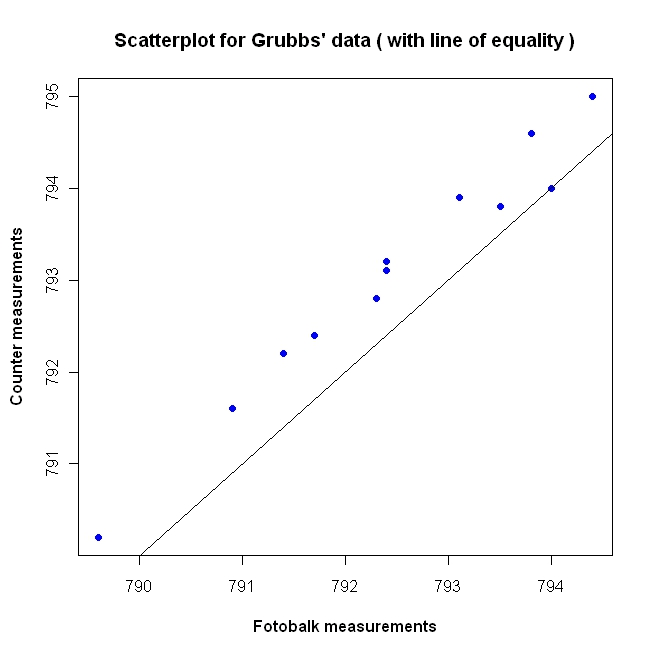
\includegraphics[width=125mm]{images/GrubbsScatter.jpeg}
			\caption{Scatter plot for Fotobalk and Counter methods.}\label{GrubbsScatter}
		\end{center}
	\end{figure}
	% %	\section{Variations and Alternative Graphical Methods}
	%In this section, we will look at some variations and enhancements of the Bland-Altman plot, as well as some alternative graphcial techniques. 
	% %	Strictly speaking, 
	%%The Identity Plot is advised by Bland and Altman as a prior analysis to the Bland-Alman plot, and therefore is neither a variant nor an alternative approach. 
	
	%========================================================= %
	
	
	The Bland-Altman plot for comparing the `Fotobalk' and `Counter' methods, which shall henceforth be referred to as the `F vs C' comparison, is depicted in Figure ~\ref{GrubbsBA-noLOA}, using data from Table~\ref{GrubbsData1}. The dashed line in Figure ~\ref{GrubbsBA-noLOA} alludes to the inter-method bias between the two methods, as mentioned previously. Bland and Altman recommend the estimation of inter-method bias by calculating the	average of the differences. In the case of Grubbs data the inter-method bias is $-0.6083$ metres per second.
	
	
	
	By inspection of the plot, it is also possible to compare the precision of each method. Noticeably the differences tend to increase as the averages increase.
	
	
	\begin{table}[h!]
		\renewcommand\arraystretch{0.7}%
		\begin{center}
			\begin{tabular}{|c||c|c||c|c|}
				\hline
				Round & Fotobalk  & Counter  & Differences  & Averages  \\
				&  [F] & [C] & [F-C] &  [(F+C)/2] \\
				\hline
				1 & 793.8 & 794.6 & -0.8 & 794.2 \\
				2 & 793.1 & 793.9 & -0.8 & 793.5 \\
				3 & 792.4 & 793.2 & -0.8 & 792.8 \\
				4 & 794.0 & 794.0 & 0.0 & 794.0 \\
				5 & 791.4 & 792.2 & -0.8 & 791.8 \\
				6 & 792.4 & 793.1 & -0.7 & 792.8 \\
				7 & 791.7 & 792.4 & -0.7 & 792.0 \\
				8 & 792.3 & 792.8 & -0.5 & 792.5 \\
				9 & 789.6 & 790.2 & -0.6 & 789.9 \\
				10 & 794.4 & 795.0 & -0.6 & 794.7 \\
				11 & 790.9 & 791.6 & -0.7 & 791.2 \\
				12 & 793.5 & 793.8 & -0.3 & 793.6 \\
				\hline
			\end{tabular}
			\caption{Fotobalk and Counter methods: Differences and Averages.}
			\label{GrubbsData1}
		\end{center}
	\end{table}
	
	\begin{table}[h!]
		\renewcommand\arraystretch{0.7}%
		\begin{center}
			\begin{tabular}{|c||c|c||c|c|}
				\hline
				Round & Fotobalk  & Terma  & Differences  & Averages  \\
				&  [F] & [T] & [F-T] &  [(F+T)/2] \\
				\hline
				1 & 793.8 & 793.2 & 0.6 & 793.5 \\
				2 & 793.1 & 793.3 & -0.2 & 793.2 \\
				3 & 792.4 & 792.6 & -0.2 & 792.5 \\
				4 & 794.0 & 793.8 & 0.2 & 793.9 \\
				5 & 791.4 & 791.6 & -0.2 & 791.5 \\
				6 & 792.4& 791.6 & 0.8 & 792.0 \\
				7 & 791.7 & 791.6 & 0.1 & 791.6 \\
				8 & 792.3 & 792.4 & -0.1 & 792.3 \\
				9 & 789.6 & 788.5 & 1.1 & 789.0 \\
				10 & 794.4 & 794.7 & -0.3 & 794.5 \\
				11 & 790.9 & 791.3 & -0.4 & 791.1 \\
				12 & 793.5 & 793.5 & 0.0 & 793.5 \\
				
				\hline
			\end{tabular}
			\caption{Fotobalk and Terma methods: Differences and Averages.}
			\label{GrubbsData2}
		\end{center}
	\end{table}
	
	\newpage
	
	\begin{figure}[h!]
		\begin{center}
			\includegraphics[width=90mm]{images/GrubbsBAplot-noLOA.jpeg}
			\caption{Bland-Altman plot For Fotobalk and Counter methods.}\label{GrubbsBA-noLOA}
		\end{center}
	\end{figure}
	
	
	
	In Figure 1.3 Bland-Altman plots for the `F vs C' and `F vs T'
	comparisons are shown, where `F vs T' refers to the comparison of
	the `Fotobalk' and `Terma' methods. Usage of the Bland-Altman plot
	can be demonstrate in the contrast between these comparisons. By inspection, there exists a larger inter-method bias in the `F vs C' comparison than in the `F vs T' comparison. Conversely there
	appears to be less precision in `F vs T' comparison, as indicated
	by the greater dispersion of covariates.
	
	\begin{figure}[h!]
		\begin{center}
			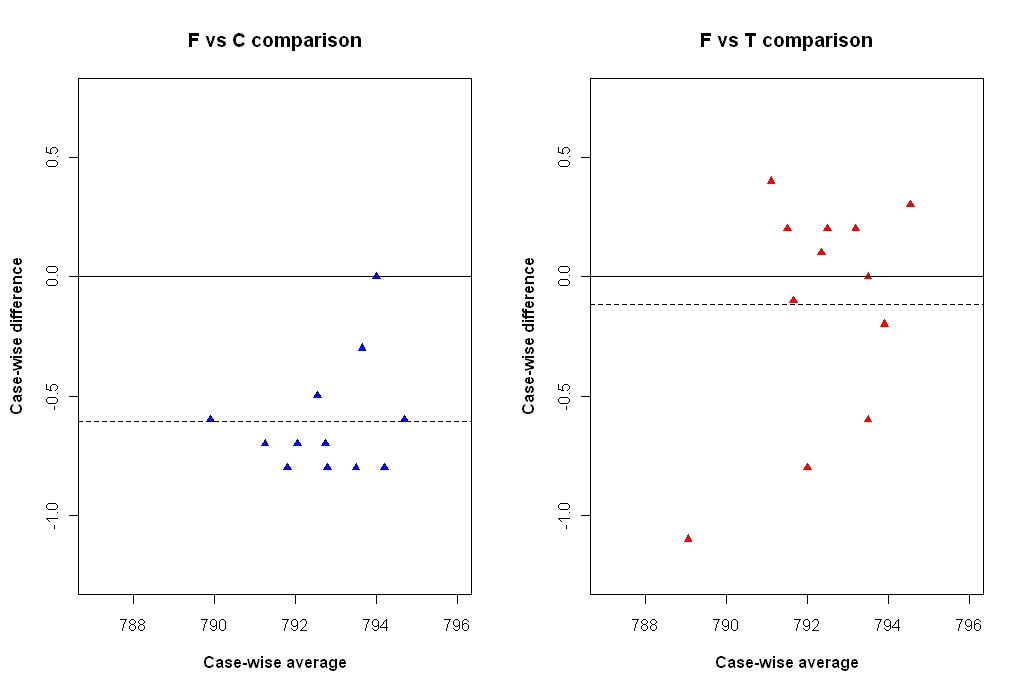
\includegraphics[height=100mm]{images/GrubbsDataTwoBAplots.jpeg}
			\caption{Bland-Altman plots for Grubbs' F vs C and F vs T comparisons.}\label{GrubbsDataTwoBAplots}
		\end{center}
	\end{figure}
	
	
	
	
	%\subfile{TechAcceptModel.tex}
	
	
	%\begin{figure}[h!]
	%	\begin{center}
	%		\includegraphics[width=120mm]{GrubbsBAplot-noLOA.jpeg}
	%		\caption{Bland-Altman plot For Fotobalk and Counter methods.}\label{GrubbsBA-noLOA}
	%	\end{center}
	%\end{figure}
	
	
	
	%	\section{scatter plots} The authors advise the
	%	use of scatter plots to identify outliers, and to determine if
	%	there is curvilinearity present. In the region of linearity
	%	,simple linear regression may yield results of interest.
	
	
	
	\subsection{Inspecting the Data}
	
	Estimates for inter-method bias and variance of differences are only meaningful if there is uniform inter-bias and variability throughout the range of measurements. Fulfilment of these assumptions can be checked by visual inspection of the plot.
	
	% % The prototype Bland-Altman plots depicted in Figures 1.4, 1.5 and 1.6 are derived from simulated data, for the purpose of demonstrating how the plot would inform an analyst of features that would adversely affect use of the recommended approach.
	
	Figures~\ref{BAFanEffect},~\ref{PropBias} and ~\ref{BAOutliers} are three Bland-Altman plots derived from
	simulated data, each for the purpose of demonstrating how the plot would inform an analyst of trends that would adversely affect use of the recommended methodology. Figure~\ref{BAFanEffect} demonstrates how the Bland-Altman plot would indicate
	increasing variance of differences over the measurement range.
	Fitted regression lines, for both the upper and lower half of the	plot, have been added to indicate the trend. Application of regression techniques to the Bland-Altman plot, and subsequent formal testing for the constant variability of differences is informative. The data set may be divided into two subsets, containing the observations wherein the difference values are less than and greater than the inter-method bias respectively. For both of these fits, hypothesis tests for the respective slopes can be performed. While both tests could be considered separately, multiple comparison procedures, such as the Benjamini-Hochberg \citep{BH} test, are advisable.
	
	Figure ~\ref{PropBias} is an example
	of cases where the inter-method bias changes over the measurement range. This is known as proportional bias, and is defined by \citet{ludbrook97} as meaning that `one method gives
	values that are higher (or lower) than those from the other by an
	amount that is proportional to the level of the measured variable'. Both of these cases violate the assumptions necessary for further analysis using limits of agreement, which shall be discussed later. 
	
	\begin{figure}[h!]
		\begin{center}
			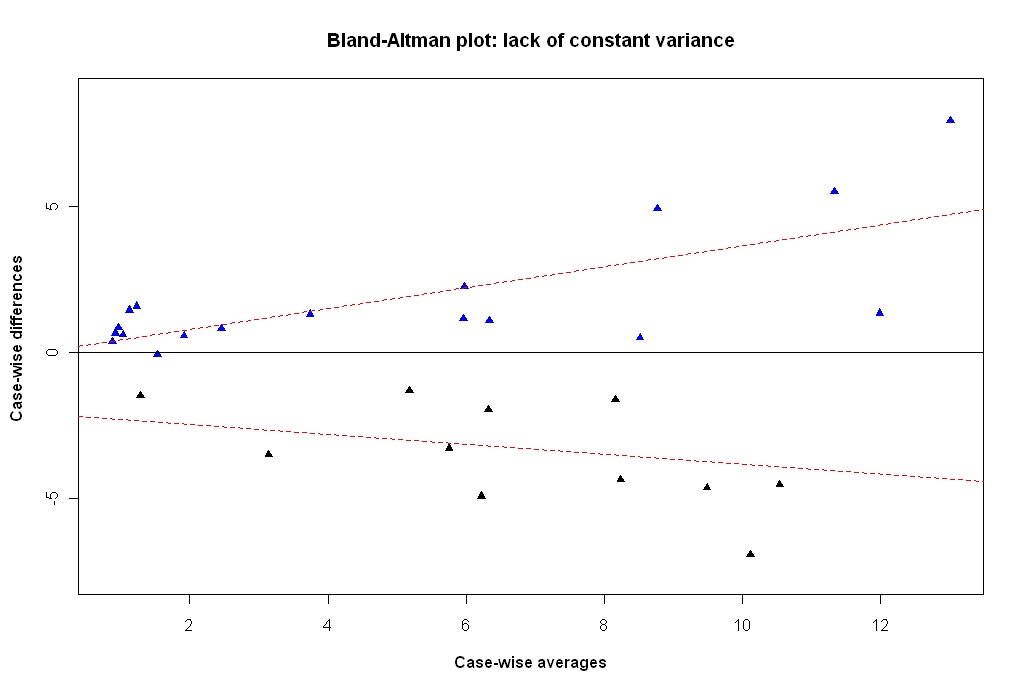
\includegraphics[width=110mm]{images/BAFanEffect.jpeg}
			\caption{Bland-Altman Plot demonstrating the increase of variance over the range}\label{BAFanEffect}
		\end{center}
	\end{figure}
	
	\begin{figure}[h!]
		\begin{center}
			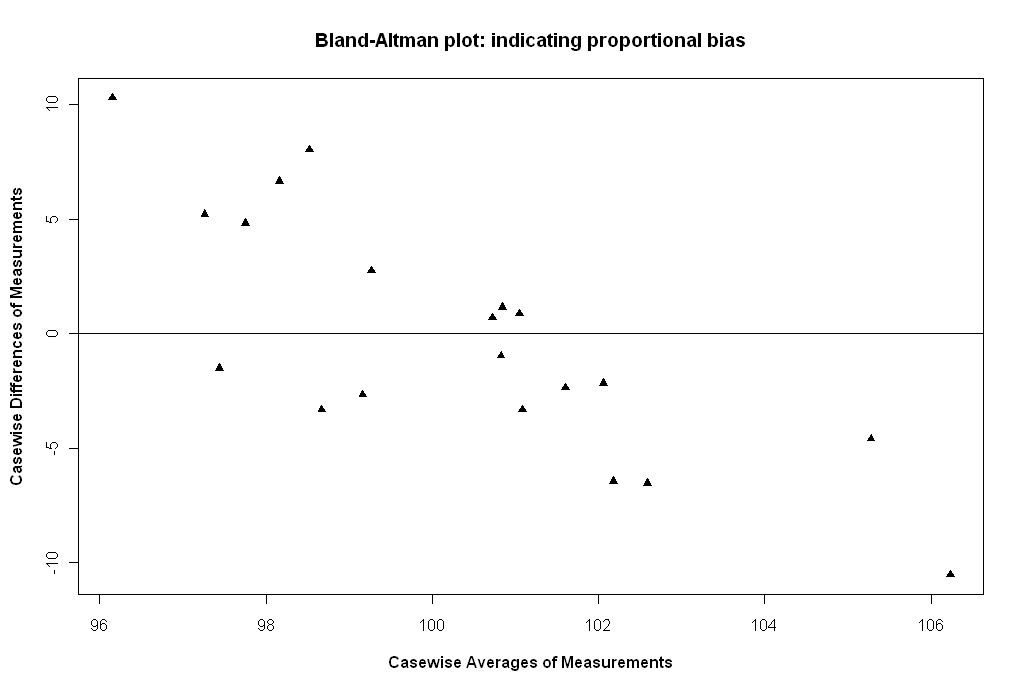
\includegraphics[width=110mm]{images/PropBias.jpeg}
			\caption{Bland-Altman Plot indicating the presence of proportional bias}\label{PropBias}
		\end{center}
	\end{figure}
	
	
	\subsection{Limits of Agreement}
	% introduces
	A third element of the Bland-Altman methodology, an interval known
	as `limits of agreement' is introduced in \citet*{BA86}
	(sometimes referred to in literature as 95\% limits of agreement). Bland and Altman proposed a pair of Limits of agreement. These
	limits are intended to demonstrate the range in which 95\% of the
	sample data should lie. The Limits of agreement centre on the
	average difference line and are 1.96 times the standard deviation
	above and below the average difference line.
	
	
	
	For the Grubbs `F vs C' comparison, these limits
	of agreement are calculated as -0.132 for the upper bound, and
	-1.08 for the lower bound. Figure ~\ref{GrubbsBAplot-noLOA} shows the resultant
	Bland-Altman plot, with the limits of agreement shown in dotted.
	
	
	\begin{figure}[h!]
		\begin{center}
			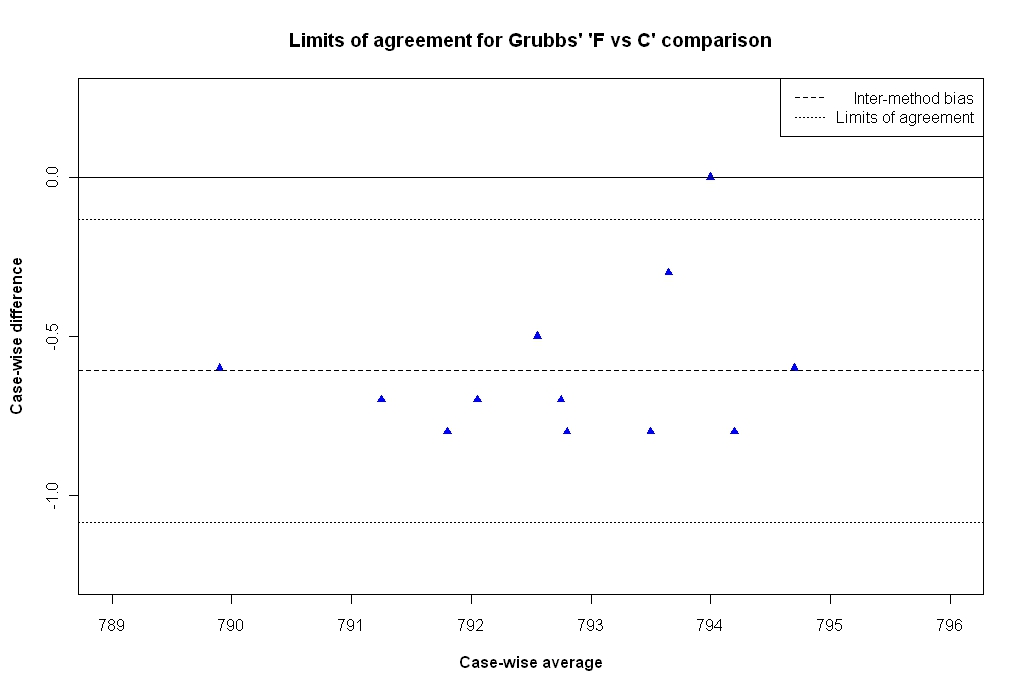
\includegraphics[width=125mm]{images/GrubbsBAplot-LOA.jpeg}
			\caption{Bland-Altman plot with limits of agreement}
			\label{GrubbsBAplot-noLOA}
		\end{center}
	\end{figure}
	
	Limits of agreement are used to assess whether the two methods of
	measurement can be used interchangeably, by demonstrating the range in which 95\% of the sample data should lie. Following basic principles of the normal probability distribution, the Limits of Agreement are centred on the average difference line (which indicates the inter-method bias) and are 1.96 times the standard deviation
	above and below the average difference line. The limits of agreement methodology assumes a constant level of bias throughout the range of measurements. 
	
	\citet{BA86} refer to
	this as the `equivalence' of two measurement methods. The specific purpose of the limits of
	agreement must be
	established clearly. \citet*{BA95} comment that the limits of agreement `\textit{how
		far apart measurements by the two methods were likely to be for
		most individuals}', a definition echoed in their 1999 paper:
	
	\begin{quote}"We can then say that nearly all pairs
		of measurements by the two methods will be closer together than
		these extreme values, which we call 95\% limits of agreement.
		These values define the range within which most differences
		between measurements by the two methods will lie."
	\end{quote}
	
	The limits of agreement (LOA) are computed by the following
	formula:
	\[
	LOA = \bar{d} \pm 1.96 s_{d}
	\]
	with $\bar{d}$ as the estimate of the inter method bias, $s_{d}$
	as the standard deviation of the differences and 1.96 is the 95\%
	quantile for the standard normal distribution. 
	% (Some descriptions of the Bland-Altman plot use 2 standard deviations instead for simplicity.)
	
	Importantly the authors recommend prior determination of what would constitute acceptable agreement, and that sample sizes should be predetermined to give an accurate conclusion. However, \citet{mantha} highlight inadequacies in the correct application of limits of agreement, resulting in contradictory estimates of limits of agreement in various papers.
	
	
	
	
	
	%========================================================== %
	
	
	
	\subsection{Normality of Case-wise Differences}	
	The difference are assumed to be normally distributed, although the measurements themselves are not assumed to follow any distribution. Therefore the authors argue that the 95\% of differences are expected to lie within these limits. 
	
	Calculation of the limits of agreement relies on the assumption that the case-wise differences are normally distributed.
	The calculation removes a lot of the variation between subjects,  leaving measurement error, which is likely to be normally distributed. \citet{BA99} remark that this assumption is easy to check using a normal plot. 
	
	
	This assumption is justified because variation between subjects has been removed, leaving only measurement error \citep{BA86}. There are formal methodologies to test whether this assumption holds.
	
	%But as \citet*{BA86} point out this may not be the case. Variants of the limits of agreement that overcome this
	% problem shall be introduced in due course.
	
	
	
	
	
	\subsection{Interpretation of Limits Of Agreement}
	
	%
	%As \citet*{BA86} point
	%out this may not be the case. Bland and Altman advises on how to
	%calculate of confidence intervals for the inter-method bias and
	%the limits of agreement. 
	
	%\subsubsection{Small Sample Sizes} The limits of agreement are
	%estimates derived from the sample studied, and will differ from
	%values relevant to the whole population, hence the importance of a
	%suitably large sample size. A different sample would give
	%different limits of agreement. Student's t-distribution is a well
	%known probability distribution used in statistical inference for
	%normally distributed populations when the sample size is small
	%\citep{student,Fisher3}. Consequently, using 't' quantiles , as
	%opposed to standard normal quantiles, may give a more appropriate
	%calculation for limits of agreement when the sample size is small.
	%For sample size $n=12$ the `t' quantile is 2.2 and the limits of
	%agreement are (-0.074,-1.143).
	
	\citet{BA99} note the similarity of limits of agreement to
	confidence intervals, but are clear that they are not the same thing. Interestingly, they describe the limits as `\textit{being like a reference interval}', offering no elaboration.
	
	The Shewhart chart is a well known graphical
	methodology used in statistical process control. Consequently
	there is potential for misinterpreting the limits of agreement as
	if they were Shewhart control limits. Importantly the
	parameters used to determine the limits, the mean and standard
	deviation, are not based on any randomly ordered sample used for an analysis, but on a statistical process's time ordered values, a key difference with Bland-Altman limits of agreement.
	
	%\citet{BXC2008} offers an alternative, more specific,  definition of
	%the limits of agreement \emph{"a prediction interval for the
	%	difference between future measurements with the two methods on a
	%	new individual."}
	
	\citet{BXC2008} regards the limits of agreement as a prediction interval for the difference between future measurements with the two methods on a new individual, but states that it does not fit the formal definition of a prediction interval, since the
	definition does not consider the errors in estimation of the parameters. 
	
	Prediction intervals, which are often used in regression analysis, are estimates of an interval in which future
	observations will fall, with a certain probability, given what has already been observed. \citet{BXC2008} offer an alternative
	formulation, a $95\%$ prediction interval for the difference
	\begin{equation}
	\bar{d} \pm t_{(0.025, n-1)}S_{d} \sqrt{1+\frac{1}{n}}
	\end{equation}
	
	%\noindent where $n$ is the number of subjects. Only for 61 or more
	%subjects is there a quantile less than 2.
	where $n$ is the number of subjects. With consideration of the effect of the sample size on the interval
	width, \citet{BXC2008} remarks that only for 61 or more subjects is the quantile less than 2.
	
	\citet{luiz} describes limits of agreement as tolerance limits. A
	tolerance interval for a measured quantity is the interval in
	which a specified fraction of the population's values lie, with a
	specified level of confidence. \citet{luiz} offers an alternative description of limits of agreement, this time as tolerance limits. 
	
	\citet{Barnhart} describes them as a probability interval, and offers a clear description of how they should be used; `\textit{if the absolute limit is less than an acceptable difference $d_{0}$, then the agreement between the two methods is deemed satisfactory}'.
	
	Various other interpretations as to how limits of agreement should properly be defined. The prevalence of contradictory definitions of what limits of agreement strictly will inevitably attenuate the poor standard of reporting using limits of agreement, as discussed by \citet{mantha}.
	
	%At least 100 historical
	%values must be used to determine the acceptable value (i.e the
	%process mean) and the process standard deviation. The principle
	%that the mean and variance of a large sample of a homogeneous
	%population is a close approximation of the population's mean and
	%variance justifies this.
	
	
	\subsection{Criticism of Limits of Agreement }
	The Bland-Altman methodology is well noted for its ease of use, and can be easily implemented with most software packages. Also it does not require the practitioner to have more than basic statistical training. The plot is quite informative about the variability of the differences over the range of measurements. For
	example, an inspection of the plot will indicate the `fan effect'. They also can be used to detect the presence of an outlier.
	
	Limits of agreement are intended to analyse equivalence. How this is assessed is the considered judgement of the practitioner. In \citet{BA86} an example of good agreement is cited. For two
	methods of measuring `oxygen saturation', the limits of agreement are calculated as (-2.0,2.8) percentage points. An knowledgeable practitioner would ostensibly find
	this to be sufficiently narrow.
	
	If the limits of agreement are not clinically important, which is
	to say that the differences tend not to be substantial, the two
	methods may be used interchangeably. \citet{DunnSEME} takes issue
	with the notion of `equivalence', remarking that while agreement
	indicated equivalence, equivalence does not reflect agreement.
	
	%
	%
	%How this relates the overall population is unclear. It seems that
	%it depends on an expert to decide whether or not the range of
	%differences is acceptable. In a study A Bland-Altman plots compare
	%two assay methods. It plots the difference between the two
	%measurements on the Y axis, and the average of the two
	%measurements on the X axis
	
	
	If one method is sometimes higher, or sometimes lower, the average of the differences will be close to zero.
	If it is not close to zero, this indicates that the two assay methods are producing different results systematically.
	
	Several problems have been highlighted regarding Limits of Agreement. One is the somewhat arbitrary manner in which they are
	constructed. While in essence they are similar to confidence intervals, they are not constructed as such; they are designed for future values.
	\citet{ludbrook97,ludbrook02} criticizes Bland-Altman plots on the
	basis that they present no information on effect of constant bias
	or proportional bias. These plots are only practicable when both
	methods measure in the same units, hence they are totally
	unsuitable for conversion problems. The limits of agreement are
	somewhat arbitrarily constructed. They may or may not be suitable
	for the data in question. It has been found that the limits given
	are too wide to be acceptable. There is no guidance on how to deal
	with outliers. Bland and Altman recognize the effect they would have
	on the limits of agreement, but offer no guidance on how to
	correct for those effects.	
	
	
	\section{Detection of Outliers}
	%As with the Bland-Altman plot, the formulation of the Limits of Agreement is also heavily influenced by outliers. An example
	%in \citet*{BA83} demonstrates the effect of recalculating without
	%a particular outlier. Refering to the VCF data set in the same
	%paper, there is more than one outlier.
	
	The Bland-Altman plot also can be used to identify outliers. An outlier is an observation that is conspicuously different from the rest of the data that it arouses suspicion that it occurs due to a mechanism, or conditions, different to that of the rest of the observations. In their 1983 paper they merely state that the plot can be used to
	``spot outliers". In their 1986 paper, Bland and Altman give an example of an
	outlier. They state that it could be omitted in practice, but make
	no further comments on the matter. In \citet{BA99}, we get the clearest indication of
	what they suggest on how to react to the presence of
	outliers. Their recommendation is to recalculate the limits
	without them, in order to test the difference with the calculation
	where outliers are retained. \citet*{BA99} do not recommend excluding outliers from analyses. However recalculation of the inter-method bias estimate, and further calculations based upon that estimate, are useful for assessing the influence of outliers. \citet{BA99} states that \emph{``We usually find that this method of analysis is not too sensitive to one or two large outlying differences."}
	Classification thereof is a subjective decision in any analysis, but must be informed by the logic of the formulation. Figure ~\ref{BAOutliers} is a Bland Altman plot with two
	conspicuous observations, at the extreme left and right of the
	plot respectively. Importantly, outlier classification must be informed by the logic of the mechanism that produces the data.
	
	%Figure ~\ref{BAOutliers} demonstrates how the Bland-Altman plot can be used to visually inspect the presence of potential outliers.
	
	
	
	\begin{figure}[h!]
		\begin{center}
			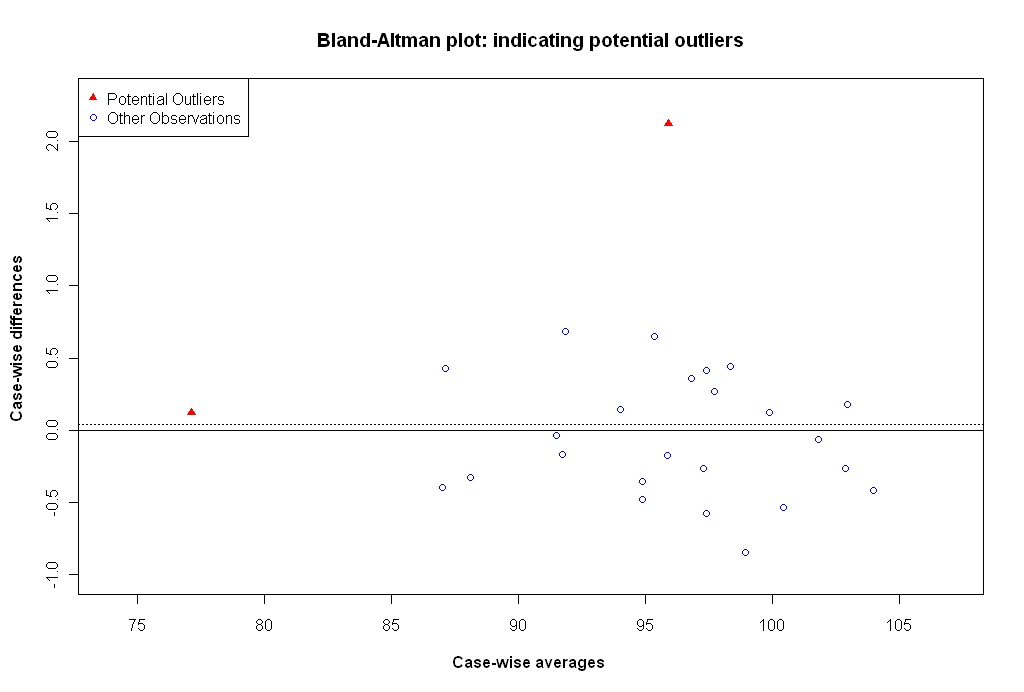
\includegraphics[width=125mm]{images/BAOutliers.jpeg}
			\caption{Bland-Altman plot indicating the presence of outliers}\label{BAOutliers}
		\end{center}
	\end{figure}
	
	
	In the Bland-Altman plot, the horizontal displacement of any observation is supported by two independent measurements. Hence any observation, such as the one on the extreme right of figure~\ref{BAOutliers}, should not be considered an outlier on the basis of a noticeable horizontal displacement from the main cluster. 
	
	The one	on the extreme left should be considered an outlier, as it has a noticeable vertical displacement from the rest of the observations. Conversely, the fourth observation from the original data set should be considered an outlier, as it has a noticeable vertical displacement from the rest of the observations.
	
	\subsection{Bartko's Ellipse}
	
	As an enhancement on the Bland Altman Plot, \citet{Bartko} has
	expounded a confidence ellipse for the covariates. \citet{Bartko} offers a graphical complement to the Bland-Altman
	plot in the form of a bivariate confidence ellipse as a boundary for dispersion. \citet{AltmanEllipse} provides the relevant calculations for the ellipse. This ellipse is intended as a visual
	guideline for the scatter plot, for detecting outliers and to
	assess the within- and between-subject variability. The stated purpose is to `amplify dispersion', which presumably is for the purposes of outlier detection. The orientation of the the ellipse is key to interpreting the results.
	Additionally Bartko's ellipse provides a visual aid to determining the
	relationship between variances. 
	
	
	%\citet{AltmanEllipse} provides the relevant calculations.
	
	\begin{figure}[h!]
		% Requires \usepackage{graphicx}
		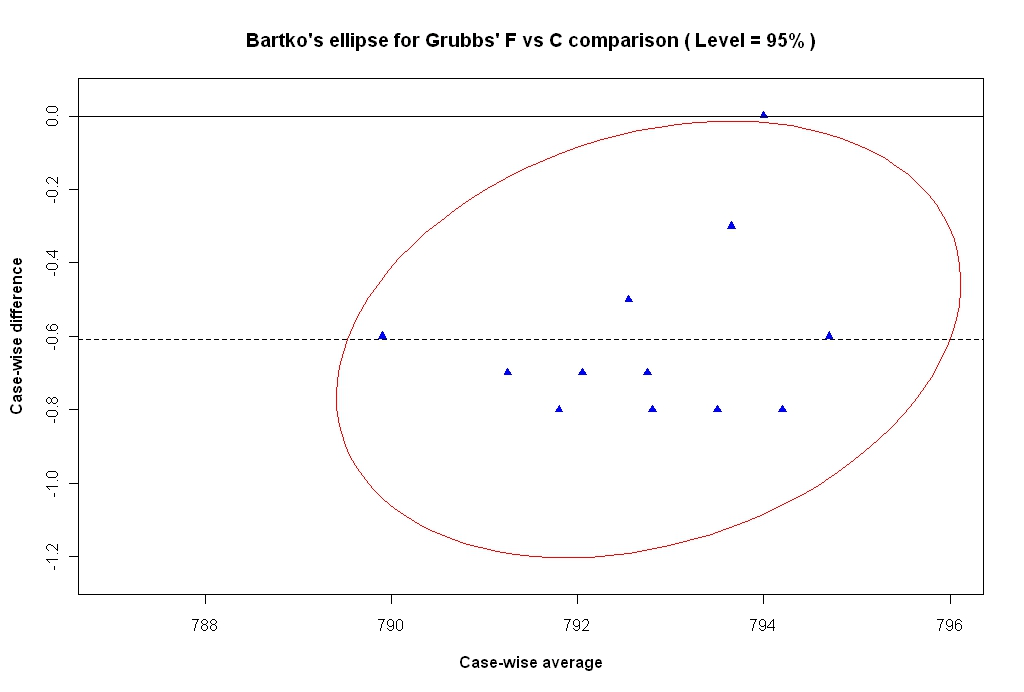
\includegraphics[width=130mm]{images/GrubbsBartko.jpeg}
		\caption{Bartko's ellipse for Grubbs data}\label{GrubbsBartko}
	\end{figure}
	
	The minor axis relates to the between-subject variability, whereas the major axis relates to the error mean square, with the ellipse depicting the size of both relative to each other.
	
	Furthermore, the ellipse provides a visual aid to determining the relationship between the variance of the means $\operatorname{var}(a)$ and the variance of the differences $\operatorname{var}(d)$. If $\operatorname{var}(a)$ is greater than $\operatorname{var}(d)$, the orientation of the ellipse is horizontal. Conversely if $\operatorname{var}(a)$ is less than $\operatorname{var}(d)$, the orientation of the ellipse is vertical. The more horizontal the ellipse, the greater the degree of agreement between the two methods being tested.
	
	
	%(Furthermore \citet{Bartko}
	%proposes formal testing procedures, that shall be discussed in due
	%course.)
	Bartko states that the ellipse can, inter alia, be used to detect the presence of outliers. The limitations of using bivariate approaches to outlier detection in the Bland-Altman plot can demonstrated using Bartko's ellipse.
	
	
	The Bland-Altman plot for the Grubbs data, complemented by Bartko's ellipse, is depicted in figure~\ref{GrubbsBartko}.
	The fourth observation is shown to be outside the bounds of the ellipse, indicating that it is a potential outlier.
	
	A covariate is added to the `F vs C' comparison that has a difference value equal to the inter-method bias, and an average value that markedly deviates from the rest of the average values
	in the comparison, i.e. 786. Figure~\ref{GrubbsBartko2} depicts a $95\%$ confidence
	ellipse for this manipulated data set. By inspection of the confidence interval, we would conclude that this extra covariate is an outlier, in spite of the fact that this observation is very close to the inter-method bias as determined by this approach.
	
	\begin{figure}[h!]
		% Requires \usepackage{graphicx}
		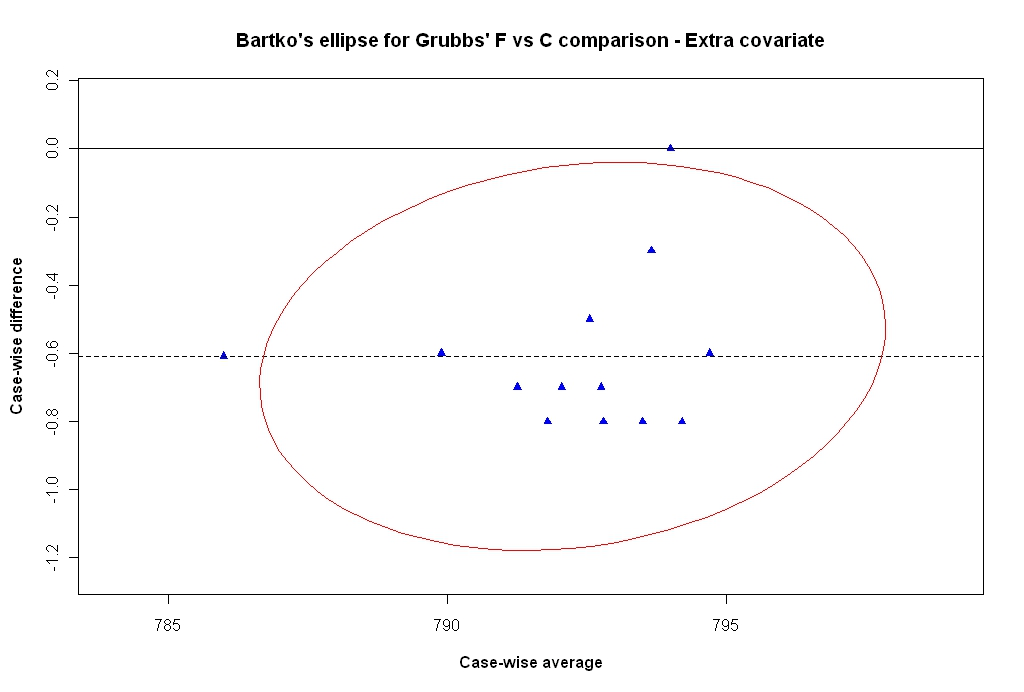
\includegraphics[width=130mm]{images/GrubbsBartko2.jpeg}
		\caption{Bartko's Ellipse for Grubbs' data, with an extra covariate.}\label{GrubbsBartko2}
	\end{figure}
	
	
	%----------------------------------------------------------------------------%
	\subsection{Grubbs' Test for Outliers}
	
	In classifying whether an observation from a univariate data set is an outlier, many formal tests are available, such as the Grubbs test for outliers. In assessing whether a covariate in a Bland-Altman plot is an outlier, this test is useful when applied to the case-wise difference values treated as a univariate data set. The null hypothesis of the Grubbs test procedure is the absence of any outliers in the data set. 
	
	The test statistic for the Grubbs test ($G$) is the largest absolute deviation from the sample mean divided by the standard
	deviation of the differences,
	\begin{equation}
	G =  \displaystyle\max_{i=1,\ldots, n}\frac{\left \vert d_i -
		\bar{d}\right\vert}{S_{d}}.
	\end{equation}
	
	For the `F vs C' comparison it is the fourth observation that gives rise to the test statistic, $G = 3.64$. The critical value is
	calculated using Student's $t$ distribution and the sample size,
	\[
	U = \frac{n-1}{\sqrt{n}} \sqrt{\frac{t_{\alpha/(2n),n-2}^2}{n - 2
			+ t_{\alpha/(2n),n-2}^2}}.
	\]
	For this test $U = 0.75$. The conclusion of this test is that the fourth observation in the `F vs C' comparison is an outlier, with $p-$value = 0.003, in accordance with the previous result of Bartko's ellipse.
	
	
	%========================================================================================== %
	
	
	
	
	
	
	
	\section{Precision of Limits of Agreement}
	
	The limits of agreement are estimates derived from the sample studied, and will differ from values relevant to the whole
	population. \citet*{BA86} advance a formulation for confidence
	intervals of the inter-method bias and the limits of agreement, arguing that it is possible to make such estimates if it is assumed that the case-wise differences approximately follow a normal distribution. However \citet*{BA99} caution that such calculations may be `somewhat
	optimistic' if the associated assumptions are not valid. A $95\%$ confidence interval can be determined, by means of the
	\emph{t} distribution with $n-1$ degrees of freedom. For the inter-method bias, the confidence interval is simply that of a mean: $\bar{d} \pm t_{(\alpha/2,n-1)} S_{d}/\sqrt{n}$.
	
	The confidence intervals and standard error for the limits of agreement follow from the variance of the limits of agreement, which is shown to be
	
	\[
	\mbox{Var}(LOA) = \bigg(\frac{1}{n}+\frac{1.96^{2}}{2(n-1)}\bigg)s_{d}^{2}.
	\]
	
	If $n$ is sufficiently large this can be following approximation can be used
	\[
	\mbox{Var}(LOA) \approx 1.71^{2}\frac{s_{d}^{2}}{n}.
	\]
	Consequently the standard errors of both limits can be approximated as $1.71$ times the standard error of the differences.
	
	%%%%%%%%%%%%%%%%%%%%%%%%%%%%%%%%%%%%%%%%%%%%%%%%%%%%%%%%%%%%%%%%%%%%%%%%%%%%%%%%%%%%%%
	
	\section{Prevalence of the Bland-Altman plot}
	
	\citet*{BA86}, which further develops the Bland-Altman methodology,
	was found to be the sixth most cited paper of all time by \citet{BAcite}. \cite{Dewitte} reviews the use of Bland-Altman plots by examining all articles in the journal `Clinical Chemistry' between 1995 and 2001, describing the rate at which
	prevalence of the Bland-Altman plot has developed in scientific
	literature. This study concludes that use of the Bland-Altman plot increased over the years, from 8\% in 1995 to
	14\% in 1996, and 31-36\% in 2002.
	
	The Bland-Altman plot has since become the expected, and often the obligatory, approach for presenting method comparison
	studies in many scientific journals \citep{hollis}. Furthermore \citet{BritHypSoc} recommend its use in papers pertaining to
	method comparison studies for the journal of the British Hypertension Society.
	
	
	% %	\section{Bland Altman Plots In Literature}
	\citet{mantha} contains a study on the use of Bland Altman plots of 44 articles in several named journals over a two year period. 42 articles used Bland Altman's limits of agreement, while the other two used correlation and regression analyses. \citet{mantha} remark that 3 papers, from 42 mention predefined maximum width for limits of agreement that would not impair medical care.
	
	The conclusion of \citet{mantha} is that there are several inadequacies and inconsistencies in the reporting of results, and
	that more standardization in the use of Bland Altman plots is required. The authors recommend the prior determination of limits of agreement before the study is carried out. This contention is endorsed by \citet{lin}, which makes a similar recommendation for the sample size, noting that\emph{``sample sizes required either was 	not mentioned or no rationale for its choice was given"}.
	
	\begin{quote}
		In order to avoid the appearance of ``data dredging", both the
		sample size and the (limits of agreement) should be specified and
		justified before the actual conduct of the trial. \citep{lin}
	\end{quote}
	
	\citet{Dewitte} remark that the limits of agreement should be
	compared to a clinically acceptable difference in measurements.
	%%%%%%%%%%%%%%%%%%%%%%%%%%%%%%%%%%%%%%%%%%%%%%%%%%%%%%%%%%%%%%%%%%%%%%%%%
	
	As an alternative to limits of agreement, \citet{lin2002} proposes the use of
	the mean square deviation in assessing agreement. The mean square
	deviation is defined as the expectation of the squared differences
	of two readings. The MSD is usually used for the case of two
	measurement methods $X$ and $Y$, each making one measurement for
	the same subject, and is given by:
	\[
	MSDxy = E[(x - y)^2]  = (\mu_{x} - \mu_{y})^2 + (\sigma_{x} -
	\sigma_{y})^2 + 2\sigma_{x}\sigma_{y}(1-\rho_{xy}).
	\]
	
	
	\citet{Barnhart} advises the use of a predetermined upper limit
	for the MSD value, $MSD_{ul}$, to define satisfactory agreement.
	However, a satisfactory upper limit may not be easily
	determinable, thus creating a drawback to this methodology.
	
	
	Alternative indices, proposed by \citet{Barnhart}, are the square root of the MSD and the expected absolute difference (EAD). 
	\[
	EAD = E(|x - y|) = \frac{\sum |x_{i}- y_{i}|}{n},
	\]
	Both of these indices can be interpreted intuitively, since their units are the same as that of the original measurements. They can also be compared to the maximum acceptable absolute difference between two methods of measurement $d_{0}$. For the sake of brevity, the EAD will be considered solely.
	
	The EAD can be used to supplement the inter-method bias in an
	initial comparison study, as the EAD is informative as a measure
	of dispersion, is easy to calculate and requires no distributional
	assumptions. A consequence of using absolute differences is that high variances would result in a higher EAD value. 
	
	% latex table generated in R 3.1.1 by xtable 1.7-4 package
	% Mon Feb 23 21:12:33 2015
	% latex table generated in R 3.1.1 by xtable 1.7-4 package
	% Mon Feb 23 21:13:45 2015
	% latex table generated in R 3.1.1 by xtable 1.7-4 package
	% Mon Feb 23 22:10:26 2015
	%\begin{table}[ht]
	%	\centering
	%	\begin{tabular}{r| rrrr}
	%		\hline
	%		\item & X & Y & U & V \\ 
	%		\hline
	%		1 & 101.83 & 102.52 & 98.05 & 99.53 \\ 
	%		2 & 101.68 & 102.69 & 99.17 & 96.53 \\ 
	%		3 & 97.89 & 99.01 & 100.31 & 97.55 \\ 
	%		4 & 98.15 & 99.57 & 100.35 & 96.03 \\ 
	%		5 & 99.94 & 100.85 & 99.51 & 99.00 \\ 
	%		6 & 98.85 & 98.86 & 98.50 & 100.76 \\ 
	%		7 & 99.86 & 97.85 & 100.66 & 99.37 \\ 
	%		8 & 101.57 & 100.21 & 99.66 & 108.87 \\ 
	%		9 & 100.12 & 99.85 & 99.70 & 105.16 \\ 
	%		10 & 99.49 & 98.77 & 101.55 & 94.31 \\ 
	%		\hline
	%	\end{tabular}
	%\end{table}
	
	
	
	
	\begin{table}[ht]
		\centering
		\begin{tabular}{|c|c|c|c|c|}
			\hline
			& U & V & $U-V$ & $|U-V|$ \\ 
			\hline
			1 & 98.05 & 99.53 & -1.49 & 1.49 \\ 
			2 & 99.17 & 96.53 & 2.64 & 2.64 \\ 
			3 & 100.31 & 97.55 & 2.75 & 2.75 \\ 
			4 & 100.35 & 96.03 & 4.32 & 4.32 \\ 
			5 & 99.51 & 99.00 & 0.51 & 0.51 \\ 
			6 & 98.50 & 100.76 & -2.26 & 2.26 \\ 
			7 & 100.66 & 99.37 & 1.29 & 1.29 \\ 
			8 & 99.66 & 108.87 & -9.21 & 9.21 \\ 
			9 & 99.70 & 105.16 & -5.45 & 5.45 \\ 
			10 & 101.55 & 94.31 & 7.24 & 7.24 \\ 
			\hline
		\end{tabular}
		\caption{Example data set}
		\label{EADdata}
	\end{table}
	
	To illustrate the use of EAD, consider Table ~\ref{EADdata}. The inter-method bias of 0.03, which is desirably close to zero in the context of agreement. However, an identity plot would indicate very poor agreement, as the points are noticeably distant from the line of equality.
	\begin{figure}
		\centering
		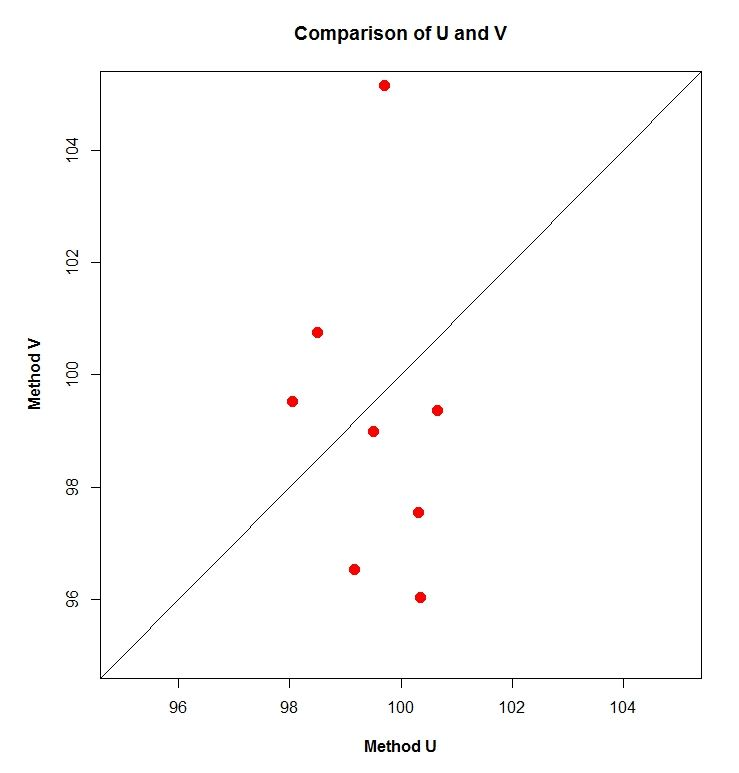
\includegraphics[width=0.5\linewidth]{EAD-UV}
		\caption{Identity Plot for example data}
		\label{fig:EADidentity}
	\end{figure}
	
	The limits of agreement are $[-9.61, 9.68]$, which is a wide interval for this data. As with the identity plot, this would indicate lack of agreement. As with inter-method bias, an EAD value close to zero is desirable. However, from Table ~\ref{EADdata}, the EAD can be computed as 3.71. The Bland-Altman plot remains a useful part of the analysis. In Figure \ref{fig:EAD1}, it is clear there is a systematic decrease in differences across the range of measurements.
	\begin{figure}[h!]
		\centering
		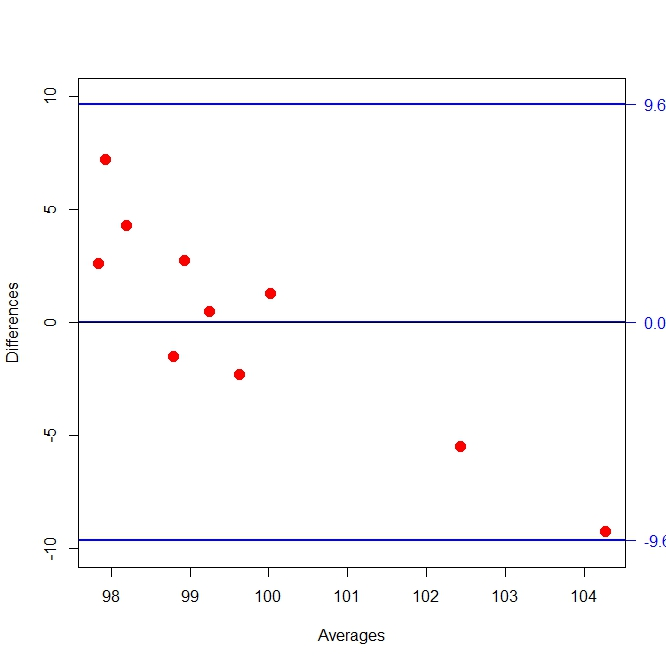
\includegraphics[width=0.55\linewidth]{images/EAD1}
		\caption{Bland-Altman Plot for UV comparison}
		\label{fig:EAD1}
	\end{figure}
	
	\citet{Barnhart} remarks that a comparison of EAD and MSD, using
	simulation studies, would be interesting, while further adding
	that `\textit{It will be of interest to investigate the benefits of these
		possible new unscaled agreement indices}'. For the Grubbs' `F vs C' and `F vs T' comparisons, the inter-method bias, difference variances, limits of agreement and EADs are shown
	in Table 1.5. The corresponding Bland-Altman plots for `F vs C' and `F vs T' comparisons were depicted previously on Figure 1.3. While the inter-method bias for the `F vs T' comparison is smaller, the EAD penalizes the comparison for having a greater variance of differences. The EAD values for both comparisons are therefore much closer.
	\begin{table}[ht]
		\begin{center}
			\begin{tabular}{|c||c|c|}
				\hline
				& F vs C & F vs T  \\\hline
				\hline
				Inter-method bias & -0.61 & 0.12 \\ \hline
				Difference variance & 0.06 & 0.22  \\ \hline 
				Limits of agreement & (-1.08,	-0.13) & (-0.81,1.04) \\ \hline
				EAD & 0.61 & 0.35  \\ \hline 
			\end{tabular}
			\caption{Agreement indices for Grubbs' data comparisons.}
		\end{center}
	\end{table}
	
	Further to  \citet{lin2000} and \citet{lin2002}, individual agreement between two measurement methods may be
	assessed using the the coverage probability (CP) criteria or the total deviation index (TDI). If $d_{0}$ is predetermined as the maximum acceptable absolute difference between two methods of measurement, the probability that the absolute difference of two measures being less than $d_{0}$ can be computed. This is known as the coverage probability (CP).
	\begin{equation}
	CP = P(|x_{i} - y_{i}| \leq d_{0})
	\end{equation}
	
	If $\pi_{0}$ is set as the predetermined coverage probability, the
	boundary under which the proportion of absolute differences is
	$\pi_{0}$ may be determined. This boundary is known as the `Total Deviation Index' (TDI). Hence the TDI is the $100\pi_{0}$
	percentile of the absolute difference of paired observations.
	%----------------------------------------------------------------------------%
	
	\section{Variations of the Bland-Altman Plot} 
	The limits of agreement methodology assumes a constant level of bias throughout the range of measurements. As \citet*{BA86} point out this may not be the case. 
	Importantly \citet{BA99} makes the following point:
	\begin{quote}These estimates are meaningful only if we can assume
		bias and variability are uniform throughout the range of
		measurement, assumptions which can be checked graphically.
	\end{quote}
	
	The importance of this statement is that, should the Bland Altman plot indicate that these assumptions are not met, then their
	entire methodology, as posited thus far, is inappropriate for use
	in a method comparison study. Again, in the context of potential
	outlier in the Grubbs data (figure 1.2), this raises the question
	on how to correctly continue. 
	
	Due to limitations of the conventional difference plot, a series of alternative formulations for the Bland-Altman approach have been proposed. Referring to the assumption that bias and variability are constant across the range of measurements, \citet{BA99} address the case where there is an increase in variability as the magnitude increases. They remark that it is possible to ignore the issue altogether, but the limits of agreement would be wider apart than necessary when just lower magnitude measurements are considered. Conversely the limits would be too narrow should only higher magnitude measurements be used. 
	
	To address the issue, they propose the logarithmic transformation of the data. The plot is then formulated as the difference of paired log values against their mean. Bland and Altman acknowledge that this is not easy to interpret, and may not be suitable in all cases.
	
	\citet{BA99} offers two variations of the Bland-Altman plot that are intended to overcome potential problems that the conventional plot would be inappropriate for. The first variation is a plot of case-wise differences as percentage of averages, and is appropriate when there is an increase in variability of the differences as the magnitude increases. 
	
	The second variation is a plot of case-wise ratios as percentage of averages, removing the need for logarithmic transformation. This approach is useful when there is an increase in variability of the differences as the magnitude of the measurement increases. \citet{Eksborg} proposed such a ratio plot, independently of Bland and Altman. \citet{Dewitte} commented on the reception of this article by saying `\textit{Strange to say, this report has been overlooked}'.
	
	
	\section{Limits of Agreement for Replicate Measurements}
	
	Computing limits of agreement features prominently in many method comparison studies since the publication of \citet{BA86}.
	\citet{BA99} addresses the issue of computing LOAs in the presence of replicate measurements, suggesting several computationally simple approaches. When repeated measures data are available, it is desirable to use
	all the data to compare the two methods. However, the original Bland-Altman method was developed for two sets of measurements done on one occasion, and so this approach is not suitable for replicate measures data. However, as a naive analysis, it may be used to explore the data because of the simplicity of the method.
	In addition to \citet{BA99}, \citet{BXC2008} computes the limits of agreement to the case with replicate measurements by using LME models. This approach will be discussed in due course.
	
	
	\section{Coefficient of Repeatability}
	
	
	\citet{BA99} strongly recommends the simultaneous estimation of repeatability and agreement by  collecting replicated data. \citet{ARoy2009} notes the lack of convenience in such calculations. The coefficient of repeatability is a measure of how well a measurement method agrees with itself over replicate measurements \citep{BA99}. 
	
	As mentioned previously, \citet{Barnhart} emphasize the importance of repeatability as part of an overall method comparison study. The coefficient of repeatability was proposed by \citet{BA99}, and is referenced in subsequent papers, such as \citet{BXC2008}. \citet{BSIrepeat} define a coefficient of
	repeatability as \emph{the value below which the difference between two single test results....may be expected to lie within a specified probability.} \citet{BA99} defines the repeatability coefficient as the upper limits of a prediction interval for the absolute difference between two measurements by the same method on the same item under identical circumstances. % \citep{BXC2008}.	
	
	Once the within-item variability for both methods has been estimated, the relevant calculations for the coefficients of repeatability are straightforward.
	The coefficient is calculated from the within-item variability $\sigma^2_{m}$ as  $1.96 \times \sqrt{2} \times \sigma_m$ = $2.83 \sigma_m$. For $95\%$ of subjects, two replicated measurement by the same method will be within this repeatability coefficient.
	
	
	The coefficient of repeatability may provide the basis for the formulation a formal definition of a `gold standard'. For example, by determining the ratio of the repeatability coefficient $(CR)$ to the sample mean $\bar{X}$. Advisably the sample size should specified in advance. A gold standard may be defined as the method with the lowest value of $\lambda = CR /\bar{X}$ with $\lambda < 0.1\%$. Similarly, a silver standard may be defined as the method with the lowest value of $\lambda $ with $0.1\% \leq \lambda < 1\%$. Such thresholds are solely for expository purposes.
	
	%------------------------------------------------------------%
	%
	%
	%	
	%\section{Coefficient of Repeatability}
	%The Bland Altman method offers a measurement on the repeatability of the methods. The \emph{Coefficient of Repeatability} (CR) can be calculated as 1.96 (or 2) times the standard deviations of the differences between the two measurements ($d_2$ and $d_1$).		
	%
	%
	%%		
	%%If the standard deviation of a measurement is $\sigma$ the repeatability coefficient is $2\times\sqrt{2} \sigma = 2.83\times \sigma \approx 2.8 \sigma$.
	%%		$\sigma^2_{x}$ is the within-subject variance of method $x$. The repeatability coefficient is $2.77 \sigma_{x}$ (i.e. $1.96 \times \sqrt{2} \sigma_{x}$). 
	%		
	%		The repeatability of measurement methods is calculated
	%		differently under the two models  Under the model assuming
	%		exchangeable replicates (1), the repeatability is based only on
	%		the residual standard deviation, i.e. $2.8\sigma_m$
	%	
	%	
	%	 The coefficient is calculated from the residual standard deviation (i.e. $1.96 \times \sqrt{2} \times \sigma_m$ = $2.83 \sigma_m$).
	
	
	
	
	
	
	
	
			\chapter{Linear Mixed effects Models}
			
			
			In cases where there are repeated measurements by each of the two methods on the same subjects, \citet{BA99} suggest calculating
			the mean for each method on each subject and use these pairs of means to compare the two methods. The estimate of bias will be unaffected using this approach, but the estimate of the standard deviation of the differences will be incorrect \citep{BXC2004}. \citet{BXC2004} recommends that replicate measurements for each method, but recognizes that resulting data are more difficult to analyze. To this end, \citet{BXC2004} and \citet{BXC2008} recommend the use of LME models as a suitable framework for method comparison in the case of repeated measurements.
			\citet{ARoy2009} uses an LME model approach to provide a set of formal tests for method comparison studies.
			
			Several authors, such as \citet{gkelly1985} and \citet{voelkel2005center}, recommend the use of Structural Equation Model from Method Comparison.
			Structural Equation Model provides a statistically rigourous analysis, but the approach is undermined in several ways. LME models have greater flexibility and can be adapted to any variant of the method comparison research question, whereas 
			SEM is suitable for some specific cases only. Highly complex models can be developed using SEM, but to overcome the problem of identifiability, a large quantity of data must be gathered.
			Often this is beyond what is practical in the main applications of method comparison studies, namely the medical sciences. Once simplifications are applied, there is little functional difference between SEM and LMEs.
			
			\section{Linear Mixed effects Models}
			A linear mixed effects (LME) model is a statistical model containing both fixed effects and random effects (also known as variance components). LME models are a generalization of the classical linear model, which contain fixed effects only. When the levels of factors are considered to be sampled from a population,
			and each level is not of particular interest, they are considered random quantities with associated variances.
			The effects of the levels, as described, are known as random effects. Random effects are represented by unobservable
			normally distributed random variables. Conversely fixed effects are considered non-random and the
			levels of each factor are of specific interest.
			%LME models are useful models when considering repeated measurements or grouped observations.
			
			\citet{Fisher4} introduced variance components models for use in genetical studies. Whereas an estimate for variance must take an non-negative value, an individual variance component, i.e.\ a component of the overall variance, may be negative.
			
			The methodology has developed since, including contributions from
			\citet{tippett}, who extend the use of variance components into linear models, and \citet{eisenhart}, who introduced the `mixed model' terminology and formally distinguished between mixed and random effects models. \citet{Henderson:1950} devised a methodology for deriving estimates for both the fixed effects and the random effects, using a set of equations that would become known as `mixed model equations' or `Henderson's equations'.
			LME methodology is further enhanced by Henderson's later works \citep{Henderson53, Henderson59,Henderson63,Henderson73,Henderson84a}. The key features of Henderson's work provide the basis for the estimation techniques.
			
			\citet{HartleyRao} demonstrated that unique estimates of the variance components could be obtained using maximum likelihood methods. However these estimates are known to be biased `downwards' (i.e.\ underestimated) , because of the assumption that the fixed estimates are known, rather than being estimated from the data. \citet{PattersonThompson} produced an alternative set of estimates, known as the restricted maximum likelihood (REML) estimates, that do not require the fixed effects to be known. Thusly there is a distinction the REML estimates and the original estimates, now commonly referred to as ML estimates.
			
			\subsection{Laird Ware Model} 
			\citet{LW82} provides a form of notation for notation for LME models that has since become the standard form, or the basis for more complex formulations. Due to computation complexity, linear mixed effects models have not seen widespread use until many well known statistical software applications began facilitating them. SAS Institute added PROC MIXED to its software suite in 1992 \citep{singer}. \citet{PB} described how to compute LME models in the \texttt{S-plus} environment.
			
			Linear mixed effects models (LME)
			differs from the conventional linear model in that it has both
			fixed effects and random effects regressors, and coefficients
			thereof. The notation provided here is generic, and will be adapted to accord with complex formulations that will be encountered in due course. Using Laird-Ware form, the LME model is commonly described in matrix form,
			\begin{equation}
			Y = X\beta + Zb + \epsilon
			\label{LW}
			\end{equation}
			
			\textbf{Y} is the $n
			\times 1$ response vector, where  $n$ is the number of observations. \textbf{$\beta$} is a $p \times 1$ vector of fixed $p$ effects, with the
			first element being the population mean. $X$ and $Z$ are $n \times p$ and $n \times q$ ``model matrices`` for fixed effects and random effects respectively, comprising
			$0$s or $1$s, depending on the observation is question. The vector of residuals, v\textbf{e} has
			dimension $n \times 1$. The random effects are contained in the  $q \times
			1$ vector \textbf{b}.
			
			%\subsection{ (good)Likelihood and estimation}
			
			% Likelihood is the hypothetical probability that an event that has already occurred would yield a specific outcome. Likelihood differs from probability in that probability refers to future occurrences, while likelihood refers to past known outcomes.
			
			% The likelihood function ($L(\theta)$)is a fundamental concept in statistical inference. It indicates how likely a particular population is to produce an observed sample. The set of values that maximize the likelihood function are considered to be optimal, and are used as the estimates of the parameters. For computational ease, it is common to use the logarithm of the likelihood function, known simply as the log-likelihood ($\ell(\theta)$).
			
			
			\subsection{LME Model Estimation}
			Estimation of LME models involve two complementary estimation issues'; estimating the vectors of the fixed and random effects estimates $\hat{\beta}$ and $\hat{b}$ and estimating the variance covariance matrices $D$ and $\Sigma$.
			Inference about fixed effects have become known as `estimates', while inferences about random effects have become known as `predictions'. The most common approach to obtain estimators are Best Linear Unbiased Estimator (BLUE) and Best Linear Unbiased Predictor (BLUP). For an LME model given by (\ref{LW}), the BLUE of $\hat{\beta}$ is given by
			\[\hat{\beta} = (X^\prime V^{-1}X)^{-1}X^\prime V^{-1}y,\]whereas the BLUP of $\hat{b}$ is given by
			\[\hat{b} = DZ^{\prime} V^{-1} (y-X\hat{\beta}).\]
			
			\subsubsection{Henderson's equations}
			
			Because of the dimensionality of V (i.e. $n \times n$) computing the inverse of V can be difficult. As a way around the this problem \citet{Henderson53, Henderson59,Henderson63,Henderson73,Henderson84a} offered a more simpler approach of jointly estimating $\hat{\beta}$ and $\hat{b}$.
			\cite{Henderson:1950} made the (ad-hoc) distributional assumptions $y|b \sim \mathrm{N} (X \beta + Zb, \Sigma)$ and $b \sim \mathrm{N}(0,D),$ and proceeded to maximize the joint density of $y$ and $b$
			\begin{equation}
			\left|
			\begin{array}{cc}
			D & 0 \\
			0 & \Sigma \\
			\end{array}
			\right|^{-\frac{1}{2}}
			\exp
			\left\{ -\frac{1}{2}
			\left(
			\begin{array}{c}
			b \\
			y - X \beta -Zb \\
			\end{array}
			\right)^\prime
			\left( \begin{array}{cc}
			D & 0 \\
			0 & \Sigma \\
			\end{array}\right)^{-1}
			\left(
			\begin{array}{c}
			b \\
			y - X \beta -Zb \\
			\end{array}
			\right)
			\right\},
			\label{u&beta:JointDensity}
			\end{equation}
			with respect to $\beta$ and $b,$ which ultimately requires minimizing the criterion
			\begin{equation}
			(y - X \beta -Zb)'\Sigma^{-1}(y - X \beta -Zb) + b^\prime D^{-1}b.
			\label{Henderson:Criterion}
			\end{equation}
			This leads to the mixed model equations
			\begin{equation}
			\left(\begin{array}{cc}
			X^\prime\Sigma^{-1}X & X^\prime\Sigma^{-1}Z
			\\
			Z^\prime\Sigma^{-1}X & X^\prime\Sigma^{-1}X + D^{-1}
			\end{array}\right)
			\left(\begin{array}{c}
			\beta \\
			b
			\end{array}\right)
			=
			\left(\begin{array}{c}
			X^\prime\Sigma^{-1}y \\
			Z^\prime\Sigma^{-1}y
			\end{array}\right).
			\label{Henderson:Equations}
			\end{equation}
			Using these equations, obtaining the estimates requires the inversion of a matrix
			of dimension $p+q \times p+q$, considerably smaller in size than $V$. \citet{Henderson63} shows that these mixed model equations do not depend on normality and that $\hat{\beta}$ and $\hat{b}$ are the BLUE and BLUP under general conditions, provided $D$ and $\Sigma$ are known.
			
			\cite{Robi:BLUP:1991} points out that although \cite{Henderson:1950} initially referred to the estimates $\hat{\beta}$ and $\hat{b}$ from (\ref{Henderson:Equations}) as ``joint maximum likelihood estimates", \cite{Henderson:1973} later advised that these estimates should not be referred to as ``maximum likelihood" as the function being maximized in (\ref{Henderson:Criterion}) is a joint density rather than a likelihood function. \cite{YLee} remarks that it is clear that Henderson used joint estimation for computational purposes, without recognizing the theoretical implications.
			
			
			
			
			
			%========================================================================================%
			
			
			
			\subsubsection{Estimation of the fixed parameters}
			
			The vector $y$ has marginal density $y \sim \mathrm{N}(X \beta,V),$ where $V = \Sigma + ZDZ^\prime$ is specified through the variance component parameters $\theta.$ The log-likelihood of the fixed parameters $(\beta, \theta)$ is
			\begin{equation}
			\ell (\beta, \theta|y) =
			-\frac{1}{2} \log |V| -\frac{1}{2}(y -
			X \beta)'V^{-1}(y -
			X \beta), \label{Likelihood:MarginalModel}
			\end{equation}
			and for fixed $\theta$ the estimate $\hat{\beta}$ of $\beta$ is obtained as the solution of
			\begin{equation}
			(X^\prime V^{-1}X) {\beta} = X^\prime V^{-1}y.
			\label{mle:beta:hat}
			\end{equation}
			
			Substituting $\hat{\beta}$ from (\ref{mle:beta:hat}) into $\ell(\beta, \theta|y)$ from (\ref{Likelihood:MarginalModel}) returns the \emph{profile} log-likelihood
			\begin{eqnarray*}
				\ell_P(\theta \mid y) &=& \ell(\hat{\beta}, \theta \mid y) \\
				&=& -\frac{1}{2} \log |V| -\frac{1}{2}(y - X \hat{\beta})'V^{-1}(y - X \hat{\beta})
			\end{eqnarray*}
			of the variance parameter $\theta.$ Estimates of the parameters $\theta$ specifying $V$ can be found by maximizing $\ell_P(\theta \mid y)$ over $\theta.$ These are the ML estimates.
			
			For REML estimation the \emph{restricted} log-likelihood is defined as
			\[
			\ell_R(\theta \mid y) =
			\ell_P(\theta \mid y) -\frac{1}{2} \log |X^\prime VX |.
			\]
			%\subsubsection{ (good)Likelihood estimation techniques}
			%Maximum likelihood and restricted maximum likelihood have become the most common strategies
			%for estimating the variance component parameter $\theta.$ Maximum likelihood estimation obtains
			%parameter estimates by optimizing the likelihood function.
			%To obtain ML estimate the likelihood is constructed as a function of the parameters in the specified LME model.
			% The maximum likelihood estimates (MLEs) of the parameters are the values of the arguments that maximize the likelihood function.
			
			The REML approach does not base estimates on a maximum likelihood fit of all the information, but instead uses a likelihood function derived from a data set, transformed to remove the irrelevant influences \citep{REMLDefine}.
			Restricted maximum likelihood is often preferred to maximum likelihood because REML estimation reduces the bias in the variance component by taking into account the loss of degrees of freedom that results
			from estimating the fixed effects in $\boldsymbol{\beta}$. Restricted maximum likelihood also handles high correlations more effectively, and is less sensitive to outliers than maximum likelihood.  The problem with REML for model building is that the likelihoods obtained for different fixed effects are not comparable. Hence it is not valid to compare models with different fixed effects using a likelihood ratio test or AIC when REML is used to
			estimate the model. Therefore models derived using ML must be used instead.
			
			\subsubsection{Estimation of the Random Effects}
			
			The established approach for estimating the random effects is to use the best linear predictor of $b$ from $y,$ which for a given $\beta$ equals $DZ^\prime V^{-1}(y - X \beta).$ In practice $\beta$ is replaced by an estimator such as $\hat{\beta}$ from (\ref{mle:beta:hat}) so that $\hat{b} = DZ^\prime V^{-1}(y - X \hat{\beta}).$ Pre-multiplying by the appropriate matrices it is straightforward to show that these estimates $\hat{\beta}$ and $\hat{b}$ satisfy the equations in (\ref{Henderson:Equations}).
			
			%	\subsubsection{Estimation of Fixed and Random Effects}
			%	Potentially it may be impossible to compute unique BLUE estimates for all the fixed factors in a model. This may be due to linear dependence in the model
			%	matrix \textbf{X}. 
			%	
			%	Estimation of random effects for LME models in the NLME package is accomplished through use
			%	of both EM (Expectation-Maximization) algorithms and Newton-Raphson algorithms.
			%	\begin{itemize}
			%		\item EM iterations bring estimates of the parameters into the region of the optimum very quickly, but
			%		convergence to the optimum is slow when near the optimum.
			%		\item Newton-Raphson iterations are computationally intensive and can be unstable when far from the
			%		optimum. However, close to the optimum they converge quickly.
			%		\item The LME function implements a hybrid approach, using 25 EM iterations to quickly get near the
			%		optimum, then switching to Newton-Raphson iterations to quickly converge to the optimum. \item If
			%		convergence problems occur, the ``control” argument in LME can be used to change the way the
			%		model arrives at the optimum.
			%	\end{itemize}
			%	
			
			
			
			
			
			%	\subsubsection{Likelihood and estimation}
			%	Likelihood is the hypothetical probability that an event that has
			%	already occurred would yield a specific outcome. Likelihood
			%	differs from probability in that probability refers to future
			%	occurrences, while likelihood refers to past known outcomes.
			%	
			%	
			%	Likelihood functions provide the basis for two important statistical concepts that shall be further referred to; the likelihood ratio test and the Akaike information criterion. The likelihood function, $L(\theta)$, is a fundamental concept in statistical
			%	inference. It indicates how likely a particular population is to produce an observed sample. The set of values that maximize the
			%	likelihood function are considered to be optimal, and are used as the estimates of the parameters. For computational ease, it is common to use the logarithm of the likelihood function, known simply as the log-likelihood ($\ell(\theta)$).
			%	
			%	Assuming a statistical model $f_{\theta}(y)$ parameterized by a fixed and unknown set of parameters $\theta$, the likelihood $L(\theta)$ is the probability of the observed data $y$ considered as a function of $\theta$ \citep{YLee}.
			%	
			%	\subsubsection{Likelihood-based tools}
			%	The maximum likelihood estimates (MLEs) of the parameters are the values of the arguments that maximize the likelihood function. Maximum likelihood and restricted maximum likelihood have become the most common strategies for estimating the variance component parameter $\theta.$ Maximum likelihood (ML) estimation is a well known method of
			%	obtaining estimates of unknown parameters by optimizing a likelihood function.  To obtain ML estimate the likelihood is constructed as a function of the parameters in the specified LME model. 
			%	
			%	The	likelihood function is constructed as a function of the parameters
			%	in the specified model. Models fitted by ML estimation can be compared using the likelihood ratio test. However ML is known to underestimate variance components for finite samples \citep{Demi}. 
			
			
			
			
			
			%%%%%%%%%%%%%%%%%%%%%%%%%%%%%%%%%%%%%%%%%%%%%%%%%%%%%%%%%%%%%%%%%%%%%%%%%%%%%%%% ML and REML
			
			
			\subsubsection{Algorithms for likelihood function optimization}Iterative numerical techniques are used to optimize the log-likelihood function and estimate the covariance parameters $\theta$. The procedure is subject to the constraint that $R$ and $D$ are both positive definite. The most common iterative algorithms for optimizing the likelihood function are the Newton-Raphson method, which is the preferred method, the expectation maximization (EM) algorithm and the Fisher scoring methods.
			
			The EM algorithm, introduced by \citet{EM}, is an iterative technique for maximizing complicated likelihood functions. The algorithm alternates between performing an expectation (E) step
			and the maximization (M) step. The `E' step computes the expectation of the log-likelihood evaluated using the current
			estimate for the variables. In the `M' step, parameters that maximize the expected log-likelihood, found on the previous `E' step, are computed. These parameter estimates are then used to determine the distribution of the variables in the next `E' step. The algorithm alternatives between these two steps until convergence is reached.
			
			The main drawback of the EM algorithm is its slow rate of
			convergence. Consequently the EM algorithm is rarely used entirely in LME estimation,
			instead providing an initial set of values that can be passed to
			other optimization techniques.
			
			The Newton Raphson (NR) method is the most common, and recommended technique for ML and
			REML estimation. The NR algorithm minimizes an objective function defines as $-2$ times the log likelihood for the covariance parameters $\theta$. At every iteration the NR algorithm requires the
			calculation of a vector of partial derivatives, known as the gradient, and the second derivative matrix with respect to the covariance parameters. This is known as the observed Hessian matrix. Due to the Hessian matrix, the NR algorithm is more time-consuming, but convergence is reached with fewer iterations compared to the EM algorithm. The Fisher scoring algorithm is an variant of the NR algorithm that is more numerically stable and likely to converge, but not recommended to obtain final estimates.
			
			\subsubsection{The extended Likelihood}
			
			The desire to have an entirely likelihood-based justification for estimates of random effects, in contrast to Henderson's equation, has motivated \citet[page 429]{Pawi:in:2001} to define the \emph{extended likelihood}. He remarks ``In mixed effects modelling the extended likelihood has been called \emph{h-likelihood} (for hierarchical  likelihood) by \cite{Lee:Neld:hier:1996}, while in smoothing literature it is known as the \emph{penalized likelihood} (e.g.\ \citeauthor{Gree:Silv:nonp:1994} \citeyear{Gree:Silv:nonp:1994})." The extended likelihood can be written $L(\beta,\theta,b|y) = p(y|b;\beta,\theta) p(b;\theta)$ and adopting the same distributional assumptions used by \cite{Henderson:1950} yields the log-likelihood function
			
			\begin{eqnarray*}
				\ell_h(\beta,\theta,b|y)
				& = \displaystyle -\frac{1}{2} \left\{ \log|\Sigma| + (y - X \beta -Zb)'\Sigma^{-1}( y - X \beta -Zb) \right.\\
				&  \hspace{0.5in} \left. + \log|D| + b^\prime D^{-1}b \right\}.
			\end{eqnarray*}
			Given $\theta$, differentiating with respect to $\beta$ and $b$ returns Henderson's equations in (\ref{Henderson:Equations}).
			
			\subsubsection{The LME model as a general linear model}
			Henderson's equations in (\ref{Henderson:Equations}) can be rewritten $( T^\prime W^{-1} T ) \delta = T^\prime W^{-1} y_{a} $ using
			\[
			\delta = \left(\begin{array}{c}\beta \\ b \end{array}\right),
			\ y_{a} = \left(\begin{array}{c}
			y \cr \psi
			\end{array}\right),
			\ T = \left(\begin{array}{cc}
			X & Z  \\
			0 & I
			\end{array}\right),
			\ \textrm{and} \ W = \left(\begin{array}{cc}
			\Sigma & 0  \cr
			0 &  D \end{array}\right),
			\]
			where \cite{YLee2006} describe $\psi = 0$ as quasi-data with mean $\mathrm{E}(\psi) = b.$ Their formulation suggests that the joint estimation of the coefficients $\beta$ and $b$ of the linear mixed effects model can be derived via a classical augmented general linear model $y_{a} = T\delta + \varepsilon$ where $\mathrm{E}(\varepsilon) = 0$ and $\mathrm{var}(\varepsilon) = W,$ with \emph{both} $\beta$ and $b$ appearing as fixed parameters. The usefulness of this reformulation of an LME as a general linear model will be revisited.
			
			
			% - Section 4
			%	\subsubsection{Algorithms}
			%	Maximum likelihood estimation is a method of obtaining estimates
			%	of unknown parameters by optimizing a likelihood function. The ML
			%	parameter estimates are the values of the argument that maximise
			%	the likelihood function, i.e. the estimates that make the observed
			%	values of the dependent variable most likely, given the
			%	distributional assumptions
			%	
			%	The most common iterative algorithms used for the optimization
			%	problem in the context of LMEs are the EM algoritm, fisher scoring	algorithm and NR algorithm, which \citet{west} commends as the preferred method. Parameter of the mixed model can be estimated using either ML or REML, while the AIC and the BIC can be used as measures of
			%	``goodness of fit" for particular models, where smaller values are
			%	considered preferable.
			
			
			%	A mixed model is an extension of the general linear models that
			%	can specify additional random effects terms.
			%	
			
			%--------------------------------------------------------------------%
			
			
			\section{Repeated measurements in LME models}
			
			In many statistical analyzes, the need to determine parameter estimates where multiple measurements are available on each of a set of variables often arises. Further to \citet{lam}, \citet{hamlett} performs an analysis of the correlation of replicate measurements, for two variables of interest, using LME models.
			
			Let $y_{Aij}$ and $y_{Bij}$ be the $j$th repeated observations of the variables of interest $A$ and $B$ taken on the $i$th subject. The number of repeated measurements for each variable may differ for each individual.
			Both variables are measured on each time points. Let $n_{i}$ be the number of observations for each variable, hence $2\times n_{i}$ observations in total.
			
			It is assumed that the pair $y_{Aij}$ and $y_{Bij}$ follow a bivariate normal distribution.
			\begin{eqnarray*}
				\left(
				\begin{array}{c}
					y_{Aij} \\
					y_{Bij} \\
				\end{array}
				\right) \sim \mathcal{N}(
				\boldsymbol{\mu}, \boldsymbol{\Sigma})\mbox{   where } \boldsymbol{\mu} = \left(
				\begin{array}{c}
					\mu_{A} \\
					\mu_{B} \\
				\end{array}
				\right)
			\end{eqnarray*}
			
			The matrix $\Sigma$ represents the variance component matrix between response variables at a given time point $j$.
			
			\[
			\boldsymbol{\Sigma} = \left( \begin{array}{cc}
			\sigma^2_{A} & \sigma_{AB} \\
			\sigma_{AB} & \sigma^2_{B}\\
			\end{array}   \right)
			\]
			
			$\sigma^2_{A}$ is the variance of variable $A$, $\sigma^2_{B}$ is the variance of variable $B$ and $\sigma_{AB}$ is the covariance of the two variable. It is assumed that $\boldsymbol{\Sigma}$ does not depend on a particular time point, and is the same over all time points.
			
			%------------------------------------------------------------------------------%
			
			\subsection{Formulation of the Response Vector}
			Information of individual $i$ is recorded in a response vector $\boldsymbol{y}_{i}$. The response vector is constructed by stacking the response of the $2$ responses at the first instance, then the $2$ responses at the second instance, and so on. Therefore the response vector is a $2n_{i} \times 1$ column vector.
			The covariance matrix of $\boldsymbol{y_{i}}$ is a $2n_{i} \times 2n_{i}$ positive definite matrix $\boldsymbol{\Omega}_{i}$.
			
			Consider the case where three measurements are taken by both methods $A$ and $B$, $\boldsymbol{y}_{i}$ is a $6 \times 1$ random vector describing the $i$th subject.
			\[
			\boldsymbol{y}_{i} = (y_{i}^{A1},y_{i}^{B1},y_{i}^{A2},y_{i}^{B2},y_{i}^{A3},y_{i}^{B3}) \prime
			\]
			
			The response vector $\boldsymbol{y_{i}}$ can be formulated as an LME model according to Laird-Ware form.
			\begin{eqnarray*}
				\boldsymbol{y_{i}} = \boldsymbol{X_{i}\beta}  + \boldsymbol{Z_{i}b_{i}} + \boldsymbol{\epsilon_{i}}\\
				\boldsymbol{b_{i}} \sim \mathcal{N}(\boldsymbol{0,D})\\
				\boldsymbol{\epsilon_{i}} \sim \mathcal{N}(\boldsymbol{0,R_{i}})
			\end{eqnarray*}
			
			Information on the fixed effects are contained in a three dimensional vector $\boldsymbol{\beta} = (\beta_{0},\beta_{1},\beta_{2})\prime$. For computational purposes $\beta_{2}$ is conventionally set to zero. Consequently $\boldsymbol{\beta}$ is the solutions of the means of the two methods, i.e. $E(\boldsymbol{y}_{i})  = \boldsymbol{X}_{i}\boldsymbol{\beta}$. The variance covariance matrix $\boldsymbol{D}$ is a general $2 \times 2$ matrix, while $\boldsymbol{R}_{i}$ is a $2n_{i} \times 2n_{i}$ matrix.
			
			%------------------------------------------------------------------------------%
			
			\subsection{Correlation Terms}
			
			\citet{hamlett} demonstrated how the between-subject and within subject variabilities can be expressed in terms of
			correlation terms.
			
			\[
			\boldsymbol{D} = \left( \begin{array}{cc}
			\sigma^2_{A}\rho_{A} & \sigma_{A}\sigma_{b}\rho_{AB}\delta \\
			\sigma_{A}\sigma_{b}\rho_{AB}\delta & \sigma^2_{B}\rho_{B}\\
			
			\end{array}\right)
			\]
			
			\[
			\boldsymbol{\Sigma} = \left(
			\begin{array}{cc}
			\sigma^2_{A}(1-\rho_{A}) & \sigma_{AB}(1-\delta)  \\
			\sigma_{AB}(1-\delta) & \sigma^2_{B}(1-\rho_{B}) \\
			\end{array}\right).
			\]
			
			$\rho_{A}$ describe the correlations of measurements made by the method $A$ at different times. Similarly $\rho_{B}$ describe the correlation of measurements made by the method $B$ at different times. Correlations among repeated measures within the same method are known as intra-class correlation coefficients. $\rho_{AB}$ describes the correlation of measurements taken at the same same time by both methods. The coefficient $\delta$ is added for when the measurements are taken at different times, and is a constant of less than $1$ for linked replicates. This is based on the assumption that linked replicates measurements taken at the same time would have greater correlation than those taken at different times. For unlinked replicates $\delta$ is simply $1$. \citet{hamlett} provides a useful graphical depiction of the role of each correlation coefficients.
			
			\citet{lam} used ML estimation to estimate the true correlation between the variables when the measurements are linked over time. The methodology relies on the assumption that the two variables with repeated measures follow a multivariate normal distribution. The methodology currently does not extend to any more than two cases. The MLE of the correlation takes into account the dependency among repeated measures.
			
			The true correlation $\rho_{xy}$ is repeated measurements can be considered as having two components: between subject and within-subject correlation. The usefulness of estimating repeated measure correlation coefficients is the calculation of between-method and within-method variabilities are produced as by-products.
			
			%=========================================================================================================== %
			\subsubsection{The Variance Covariance Matrix}
			The LME model can be written
			\[
			\boldsymbol{y_{i}} = \boldsymbol{X_{i}\beta} + \boldsymbol{Z_{i}b_{i}} + \boldsymbol{\epsilon_{i}},
			\]
			where $\boldsymbol{\beta}=(\beta_0,\beta_1,\beta_2)^\prime$ is a vector of fixed effects, and $\boldsymbol{X}_i$ is a corresponding $2n_i\times 3$ design matrix for the fixed effects. The random effects are expressed in the vector $\boldsymbol{b}=(b_1,b_2)^\prime$, with $\boldsymbol{Z}_i$ the corresponding $2n_i\times 2$ design matrix. The vector $\boldsymbol{\epsilon}_i$ is a $2n_i\times 1$ vector of residual terms. Random effects and residuals are assumed to be independent of each other.
			The variance matrix of \textbf{Y}, denoted \textbf{V}, is an $n \times n$ matrix that can be expressed
			as follows;
			\begin{eqnarray}
			\textbf{V}= \textrm{Var} ( \textbf{Xb} + \textbf{Zb} + \textbf{e})\\
			\textbf{V}= \textrm{Var} ( \textbf{Xb} ) + \textrm{Var} (\textbf{Zb}) +
			\textrm{Var}(\textbf{e})
			\end{eqnarray}
			
			
			$\mbox{Var}(\textbf{Xb})$ is known to be zero. The variance of the
			random effects $\mbox{Var}(\textbf{Zu})$ can be written as
			$Z\mbox{Var}(\textbf{b})Z^{T}$.
			\[
			\mathrm{var}
			\left(
			\begin{array}{c}
			b \\
			\epsilon \\
			\end{array}
			\right)
			=
			\left(
			\begin{array}{cc}
			D & 0 \\
			0 & \Sigma \\
			\end{array}
			\right)
			\]
			
			
			
			
			where $D$ and $\Sigma$ are positive definite matrices parameterized by an unknown variance component parameter vector $ \theta.$ The variance-covariance matrix for the vector of observations $y$ is given by $V = ZDZ^{\prime}+ \Sigma.$ This implies $y \sim(X\beta, V) = (X\beta,ZDZ^{\prime}+ \Sigma)$. 
			
			$\boldsymbol{R}_{i}$ is the variance covariance matrix for the residuals, i.e. the within-item sources of variation between both methods. Computational analysis of linear mixed effects models allow for the explicit analysis of both $\boldsymbol{D}$ and $\boldsymbol{R_i}$.
			The above terms can be used to express the  variance covariance matrix $\boldsymbol{\Omega}_i$ for the responses on item $i$ ,
			\[
			\boldsymbol{\Omega}_i = \boldsymbol{Z}_i \boldsymbol{D} \boldsymbol{Z}_i^{\prime} + \boldsymbol{R}_i.
			\]
			%============================================================== %
			
			It is assumed that $\boldsymbol{b}_i \sim N(0,\boldsymbol{D})$, $\boldsymbol{\epsilon}_i$ is a matrix of random errors distributed as $N(0,\boldsymbol{R}_i)$ and that the random effects and residuals are independent of each other. Assumptions made on the structures of $\boldsymbol{D}$ and $\boldsymbol{R}_i$ will be discussed in due course.
			
			The random effects are assumed to be distributed as $\boldsymbol{b}_i \sim \mathcal{N}_2(0,\boldsymbol{D})$. The between-item variance covariance matrix $\boldsymbol{D}$ is constructed as follows:
			%		\[ \boldsymbol{D} =\left(
			%		\begin{array}{cc}
			%		d^2_1  & d_{12} \\
			%		d_{12} & d^2_2 \\
			%		\end{array}
			%		\right) \]
			\[ \boldsymbol{D} = \mbox{Var}  \left[
			\begin{array}{c}
			b_1   \\
			b_2  \\
			\end{array}
			\right] =  \left(
			\begin{array}{cc}
			d^2_1  & d_{12} \\
			d_{12} & d^2_2 \\
			\end{array}
			\right) \]
			
			
			
			%============================================================%
			The distribution of the random effects is described as $\boldsymbol{b}_i \sim N(0,\boldsymbol{D})$. Similarly random errors are distributed as $\boldsymbol{\epsilon}_i \sim N(0,\boldsymbol{R}_i)$. The random effects and residuals are assumed to be independent. The variance-covariance matrix for the vector of observations $y$ is given by $V = ZDZ^{\prime}+ \Sigma.$ This implies $y \sim(X\beta, V) = (X\beta,ZDZ^{\prime}+ \Sigma)$. 
			
			
			By letting $\operatorname{var}(b) = D$ (i.e $\textbf{b} ~ N(0,\textbf{D})$), this becomes $ZDZ^{T}$. This specifies the covariance due to random
			effects. The residual covariance matrix $\operatorname{var}(e)$ is denoted as $R$, ($\textbf{e} ~ N(0,\textbf{R})$). Residual are uncorrelated,
			hence \textbf{R} is equivalent to $\sigma^{2}$\textbf{I}, where \textbf{I} is the identity matrix. The variance matrix \textbf{V}
			can therefore be written as;
			
			\begin{equation}
			\textbf{V}  = \textbf{ZDZ}^{T} + \textbf{R}
			\end{equation}
			
			
			
			
			\section{LME models in Method Comparison Studies}
			Linear mixed effects (LME) models can facilitate greater understanding of the potential causes of bias and differences in precision between two sets of measurement. Due to computation complexity, linear mixed effects models have not seen widespread use until many well known statistical software applications began facilitating them. Consequently LME approaches have seen increased use as a framework for method comparison studies in recent years (Lai $\&$ Shaio, Carstensen and Choudhary as examples)
			
			
			In part this is due to the increased profile of LME models, and furthermore the availability of capable software. 	Additionally a great understanding of residual analysis and influence analysis for LME models has been adchieved thanks to authors such as \citet{schabenberger}, \citet{Christensen}, \citet{cook86} \citet{west}, amongst others.
			
			
			Due to the prevalence of modern statistical software, \citet{BXC2008} advocates the adoption of computer based approaches to method comparison studies, allowing the use of LME models that would not have been feasible otherwise. These authors remark that modern statistical computation, such as that used for LME models, greatly improve the efficiency of
			calculation compared to previous `by-hand' approaches, as advocated in \citet{BA99}, describing them as tedious, unnecessary and `outdated'. Rather than using the `by hand' methods, estimates for required LME parameters can be read directly from program output. Furthermore, using computer approaches removes associated constraints, such as the need for the design to be perfectly balanced.
			
			
			\citet{Barnhart} sets out three criteria for two methods to be considered in agreement. Firstly that there be no significant bias. Second that there is no difference in the between-subject variabilities, and lastly that there is no significant difference in the within-subject variabilities. Roy further proposes examination of the the overall variability by considering the second and third criteria be examined jointly. Should both the second and third criteria be fulfilled, then the overall variabilities of both methods would be equal.
			
			Varying degrees of importances should be attached to each the three agreement criteria listed by \citet{Barnhart}. Between-item variance $d^2_i$ is fundamentally a measure of the variability of the item-wise means, as measured by method $i$, but it does contain limited information on the precision of that method. 
			
			For conventional method comparison problems, both methods measures the same set of items using the same unit of measurement. Convergence to equality of between-item variance inevitable as the number of items $n$ increases. Significantly different estimates for $d^2_1$ and $d^2_2$ should not be expected for any practical problem. 
			
			Therefore a violation of third criterium (i.e. different between-item variances) criterium is contingent upon, and a  
			possible consequence of, the violation of the other two agreement criteria. However, a violation of the third criterium will not occur in isolation. As noted elsewhere, the matter of inter-method bias can be easily accounted for, once detected. Both between-items and within-items variances must be calculated such that sources of variances are properly assigned, and to compute limits of agreement. However, testing the within-item criterium is the most informative analysis and therefore requires the most attention. 
			
			
			
			
			\citet{LaiShiao} views
			the uses of linear mixed effects models as an expansion on the
			Bland-Altman methodology, rather than as a replacement. 
			
			Their focus is to explain lack of agreement by means of additional covariates outside the scope of the traditional method comparison problem, which extends beyond the conventional method comparison study question. The data used for their examples is unavailable for independent use. 
			
			%	Therefore, for the sake of consistency, a data set will be simulated based on the Blood Data that will allow for extra variables, and an exploration shall be provided in the appendices.
			
			%----------------------------------------------------------------------------%
			
			
			
			
			
			
			\subsection{Roy's Methodology}
			
			For the purposes of comparing two methods of measurement, \citet{ARoy2009} presents a methodology utilizing linear mixed effects model. This methodology provides for the formal testing of inter-method bias, between-subject variability and within-subject variability of two methods. The formulation contains a Kronecker product covariance structure in a doubly multivariate setup. By doubly multivariate set up, Roy means that the information on each patient or item is multivariate at two levels, the number of methods and number of replicated measurements. Further to \citet{lam}, it is assumed that the replicates are linked over time. However it is easy to modify to the unlinked case.
			
			
			
			
			\citet{ARoy2009} proposes a suite of hypothesis tests for assessing the agreement of two methods of measurement, when replicate measurements are obtained for each item, using a LME approach. The tests are implemented by fitting a specific LME model, and three variations thereof, to the data. These three variant models introduce equality constraints that act null hypothesis cases.
			
			Two methods of measurement are in complete agreement if the null hypotheses $\mathrm{H}_1\colon \alpha_1 = \alpha_2$ and $\mathrm{H}_2\colon \sigma^2_1 = \sigma^2_2 $ and $\mathrm{H}_3\colon d^2_1= d^2_2$ hold simultaneously. \citet{ARoy2009} uses a Bonferroni correction to control the familywise error rate for tests of $\{\mathrm{H}_1, \mathrm{H}_2, \mathrm{H}_3\}$ and account for difficulties arising due to multiple testing. 
			
			A formal test for inter-method bias can be implemented by examining the fixed effects of the model. This is common to well known classical linear model methodologies. The null hypotheses, that both methods have the same mean, which is tested against the alternative hypothesis, that both methods have different means.
			The inter-method bias and necessary $t-$value and $p-$value are presented in computer output. A decision on whether the first of Roy's criteria is fulfilled can be based on these values.
			
			Importantly \citet{ARoy2009} further proposes a series of three tests on the variance components of an LME model, which allow decisions on the second and third of Roy's criteria. For these tests, four candidate LME models are constructed. The differences in the models are specifically in how the the $D$ and $\Lambda$ matrices are constructed, using either an unstructured form or a compound symmetry form. To illustrate these differences, consider a generic matrix $A$,
			
			\[
			\boldsymbol{A} = \left( \begin{array}{cc}
			a_{11} & a_{12}  \\
			a_{21} & a_{22}  \\
			\end{array}\right).
			\]
			
			A symmetric matrix allows the diagonal terms $a_{11}$ and $a_{22}$ to differ. The compound symmetry structure requires that both of these terms be equal, i.e $a_{11} = a_{22}$.
			
			The first model acts as an alternative hypothesis to be compared against each of three other models, acting as null hypothesis models, successively. The models are compared using the likelihood ratio test. Likelihood ratio tests are a class of tests based on the comparison of the values of the likelihood functions of two candidate models. LRTs can be used to test hypotheses about covariance parameters or fixed effects parameters in the context of LMEs. The test statistic for the likelihood ratio test is the difference of the log-likelihood functions, multiplied by $-2$.
			The probability distribution of the test statistic is approximated by the $\chi^2$ distribution with ($\nu_{1} - \nu_{2}$) degrees of freedom, where $\nu_{1}$ and $\nu_{2}$ are the degrees of freedom of models 1 and 2 respectively. Each of these three test shall be examined in more detail shortly.
			
			
			\subsection{Replicate measurements in Roy's paper}
			
			
			\citet{ARoy2009} uses the same definition of replicate measurement as \citet{BA99}; 	measurements taken in quick succession by the same observer using the same instrument on the same subject can be considered true replicates.
			under identical conditions. \citet{ARoy2009} notes that some measurements may not be `true' replicates, as data can not be collected in this way. In such cases, the correlation matrix on the replicates may require a different structure, such as the autoregressive order one $AR(1)$ structure. However determining MLEs with such a structure would be computational intense, if possible at all.
			
			
			
			
			
			\subsection{Test for inter-method bias}
			
			Firstly, a practitioner would investigate whether a significant inter-method bias is present between the methods. This bias is specified as a fixed effect in the LME model.  For a practitioner who has a reasonable level of competency in statistical software and undergraduate statistics (in particular simple linear regression model) this is a straight-forward procedure.
			
			% Three hypothesis tests follow from this equation.
			The presence of an inter-method bias is the source of disagreement between two methods of measurement that is most easily identified. As the first in a series of hypothesis tests, \citet{ARoy2009} presents a formal test for inter-method bias. With the null and alternative hypothesis denoted $H_1$ and $K_1$ respectively, this test is formulated as
			
			\[	\operatorname{H_1} : \mu_1 = \mu_2 ,\]
			\[	\operatorname{K_1} : \mu_1 \neq \mu_2.\]
			
			
			
			
			A formal test for inter-method bias can be implemented by examining the fixed effects of the model. This is common to well known classical linear model methodologies. The null hypotheses, that both methods have the same mean, which is tested against the alternative hypothesis, that both methods have different means.
			The inter-method bias and necessary $t-$value and $p-$value are presented in computer output. A decision on whether the first of Roy's criteria is fulfilled can be based on these values.
			
			
			%================================================================%
			
			\subsection{Roy's hypothesis tests : Roy's variability tests}
			
			Lack of agreement can also arise if there is a disagreement in overall variabilities. This lack of agreement may be due to differing between-item variabilities, differing within-item variabilities, or both. The formulation previously presented by Roy usefully facilitates a series of significance tests that assess if and where such differences arise. These tests are comprised of a formal test for the equality of between-item variances.
			The first candidate model is compared to each of the three other models successively. It is the alternative model in each of the three tests, with the other three models acting as the respective null models. The models are compared using the likelihood ratio test, a general method for comparing nested models fitted by ML \citep{Lehmann2006}.
			
			%	The first model acts as an alternative hypothesis to be compared against each of three other models, acting as null hypothesis models, successively. The models are compared using the likelihood ratio test. Likelihood ratio tests are a class of tests based on the comparison of the values of the likelihood functions of two candidate models. 
			
			
			The first test allows of the comparison the begin-subject variability of two methods. Similarly, the second test
			assesses the within-subject variability of two methods. A third test is a test that compares the overall variability of the two methods.
			
			Other important aspects of the method comparison study are consequent. The limits of agreement are computed using the results of the first model.
			
			
			%	\begin{eqnarray*}
			%		\operatorname{H_2} : g^2_1 = g^2_2 \\
			%		\operatorname{K_2} : g^2_1 \neq g^2_2
			%	\end{eqnarray*}%and a formal test for the equality of within-item variances.
			\begin{eqnarray*}
				\operatorname{H_3} : \sigma^2_1 = \sigma^2_2 \\
				\operatorname{K_3} : \sigma^2_1 \neq \sigma^2_2
			\end{eqnarray*}
			A formal test for the equality of overall variances is also presented.
			\begin{eqnarray*}
				\operatorname{H_4} : \omega^2_1 = \omega^2_2 \\
				\operatorname{K_4} : \omega^2_1 \neq \omega^2_2
			\end{eqnarray*}
			
			Two methods can be considered to be in agreement if criteria based upon these methodologies are met. Additionally Roy makes reference to the overall correlation coefficient of the two methods, which is determinable from variance estimates.
			
			Conversely, the tests of variability required detailed explanation. Each test is performed by fitting two candidate models, according with the null and alternative hypothesis respectively. The distinction between the models arise in the specification in one, or both, of the variance-covariance matrices. % A likelihood ratio test can then be used to compare these respective fits.
			%---------------------------------------------%
			
			Four candidates models are fitted to the data. These models are similar to one another, but for the imposition of equality constraints. The tests are implemented by fitting a four variants of a specific LME model to the data. For the purpose of comparing models, one of the models acts as a reference model while the three other variant are nested models that introduce equality constraints to serves as null hypothesis cases. The methodology uses a linear mixed effects regression fit using a combination of symmetric and compound symmetry (CS) correlation structure the variance covariance matrices.
			
			%============================================================================ %
			
			\subsection{Model Specification for Roy's Hypotheses Tests}
			
			%	\citet{ARoy2009} proposes a novel method using the LME model with Kronecker product covariance structure in a doubly multivariate set-up to assess the agreement between a new method and an established method with unbalanced data and with unequal replications for different subjects.
			Response for $i$th subject can be written as
			\[ y_i = \beta_0 + \beta_1x_{i1} + \beta_2x_{i2} + b_{1i}z_{i1}  + b_{2i}z_{i2} + \epsilon_i \]
			\begin{itemize}
				\item $\beta_1$ and $\beta_2$ are fixed effects corresponding to both methods. ($\beta_0$ is the intercept.)
				\item $b_{1i}$ and $b_{2i}$ are random effects corresponding to both methods.
			\end{itemize}
			
			
			
			%==============================================================================%
			
			
			
			
			In order to express Roy's LME model in matrix notation we gather all $2n_i$ observations specific to item $i$ into a single vector  $\boldsymbol{y}_{i} = (y_{1i1},y_{2i1},y_{1i2},\ldots,y_{mir},\ldots,y_{1in_{i}},y_{2in_{i}})^\prime.$ 
			
			
			%==========================================================================================%
			
			
			
			
			
			
			\subsection{Specifying the Models}
			Roy proposes a series of three tests on the variance components of an LME model. For these tests, four candidate models are constructed. 
			
			Using Roy's method, four candidate models are constructed, each differing by constraints applied to the variance covariance matrices. In addition to computing the inter-method bias, three significance tests are carried out on the respective formulations to make a judgement on whether or not two methods are in agreement.
			
			
			The difference in the models are specifically in how the the $D$ and $\Sigma$ matrices are constructed, using either an unstructured form or a compound symmetry form. The first model is compared against each of three other models successively.
			
			
			
			
			These tests are the pairwise comparison of candidate models, one formulated without constraints, the other with a constraint.
			
			
			
			
			
			
			
			\subsection{Variability Tests}
			
			
			
			
			
			Variability tests proposed by \citet{ARoy2009} affords the opportunity to expand upon Carstensen's approach. Three tests of hypothesis are provided, appropriate for evaluating the agreement between the two methods of measurement under this sampling scheme. 
			
			
			
			
			
			
			
			
			
			
			
			
			
			
			
			
			
			
			
			
			\subsubsection{Variability test 1}
			The first test determines whether or not both methods $A$ and $B$ have the same between-subject variability, further to the second of Roy's criteria.
			\begin{eqnarray*}
				H_{0}: \mbox{ }d_{1}  = d_{2} \\
				H_{A}: \mbox{ }d_{1}  \neq d_{2}
			\end{eqnarray*}
			This test is facilitated by constructing a model specifying a symmetric form for $D$ (i.e. the alternative model) and comparing it with a model that has compound symmetric form for $D$ (i.e. the null model). For this test $\boldsymbol{\hat{\Sigma}}$ has a symmetric form for both models, and will be the same for both.
			
			%---------------------------------------------%
			\subsubsection{Variability test 2}
			
			This test determines whether or not both methods have the same within-subject variability, thus enabling a decision on the third of Roy's criteria.
			\begin{eqnarray*}
				H_{0}: \mbox{ }\sigma_{1}  = \sigma_{2} \\
				H_{A}: \mbox{ }\sigma_{1}  \neq \sigma_{2}
			\end{eqnarray*}
			
			This model is performed in the same manner as the first test, only reversing the roles of $\boldsymbol{\hat{D}}$ and $\boldsymbol{\hat{\Sigma}}$. The null model is constructed a symmetric form for $\boldsymbol{\hat{\Sigma}}$ while the alternative model uses a compound symmetry form. This time $\boldsymbol{\hat{D}}$ has a symmetric form for both models, and will be the same for both.
			
			As the within-subject variabilities are fundamental to the coefficient of repeatability, this variability test likelihood ratio test is equivalent to testing the equality of two coefficients of repeatability of two methods. In presenting the results of this test, \citet{ARoy2009} includes the coefficients of repeatability for both methods.
			
			
			\subsubsection{Variability test 3}
			Roy also integrates $\mathrm{H}_2$ and $\mathrm{H}_3$ into a single testable hypothesis $\mathrm{H}_4\colon \omega^2_1=\omega^2_2,$ where $\omega^2_m = \sigma^2_m + d^2_m$ represent the overall variability of method $m.$ 		\citet{ARoy2009} further proposes examination of the the overall variability by considering the second and third criteria be examined jointly. Should both the second and third criteria be fulfilled, then the overall variabilities of both methods would be equal. An examination of this topic is useful because a method for computing Limits of Agreement follows from here.
			
			
			
			
			Disagreement in overall variability may be caused by different between-item variabilities, by different within-item variabilities, or by both.  If the exact cause of disagreement between the two methods is not of interest, then the overall variability test $H_4$ is an alternative to testing $H_2$ and $H_3$ separately.
			
			The estimated overall variance covariance matrix `Block
			$\Omega_{i}$' is the addition of estimate of the between-subject variance covariance matrix $\hat{D}$ and the within-subject variance covariance matrix $\hat{\Sigma}$.
			
			\begin{equation}
			\mbox{Block  }\Omega_{i} = \hat{D} + \hat{\Sigma}
			\end{equation}
			Overall variability between the two methods ($\Omega$) is sum of between-subject ($D$) and within-subject variability ($\Sigma$),
			\citet{ARoy2009} denotes the overall variability	as ${\mbox{Block - }\boldsymbol \Omega_{i}}$. The overall variation for methods $1$ and $2$ are given by
			
			\begin{center}
				\[\mbox{Block } \boldsymbol{\Omega}_i = \left(\begin{array}{cc}
				\omega^2_1  & \omega_{12} \\
				\omega_{12} & \omega^2_2 \\
				\end{array}  \right)
				=  \left(
				\begin{array}{cc}
				d^2_1  & d_{12} \\
				d_{12} & d^2_2 \\
				\end{array} \right)+
				\left(
				\begin{array}{cc}
				\sigma^2_1  & \sigma_{12} \\
				\sigma_{12} & \sigma^2_2 \\
				\end{array}\right)
				\]
			\end{center}
			
			The last of the variability test examines whether or not both methods have the same overall variability. This enables the joint consideration of second and third criteria.
			\begin{eqnarray*}
				H_{0}: \mbox{ }\omega_{1}  = \omega_{2} \\
				H_{A}: \mbox{ }\omega_{1}  \neq \omega_{2}
			\end{eqnarray*}
			
			The null model is constructed a symmetric form for both $\boldsymbol{\hat{D}}$ and $\boldsymbol{\hat{\Lambda}}$ while the alternative model uses a compound symmetry form for both.
			
			
			
			
			
			
			
			\section{Correlation terms}
			
			Roy's tests are complemented by the ability to the overall correlation coefficient of the two methods, which is determinable from variance estimates. Two methods can be considered to be in agreement if criteria based upon these tests are met. Inference for inter-method bias follows from well-established methods and, as such, will only be noted when describing examples.
			
			
			In addition to the variability tests, \citet{ARoy2009} advises that it is preferable that a correlation of greater than $0.82$ exist for two methods to be considered interchangeable. However if two methods fulfil all the other conditions for agreement, failure to comply with this one can be overlooked, and demonstrates that placing undue importance to it can lead to incorrect conclusions.
			
			\citet{ARoy2009} remarks that PROC MIXED only gives overall correlation coefficients, but not their variances. Similarly variance are not determinable in \texttt{R} as yet either. Consequently it is not possible to carry out inferences based on all overall correlation coefficients.
			
			
			
			
			
			
			The methodology proposed by \citet{ARoy2009} is largely based on \citet{hamlett}, which in turn follows on from \citet{lam}. Hamlett re-analyses the data of \citet{lam} to generalize their model to cover other settings not covered by the Lam method. In many cases, repeated observation are collected from each subject in sequence  and/or longitudinally.
			% \[ y_i = \alpha + \mu_i + \epsilon \]
			
			
			
			%------------------------------------------------------------------------------------%
			
			
			Aside from the fixed effects, another important difference is that Carstensen's model requires that particular assumptions be applied, specifically that the off-diagonal elements of the between-item
			and within-item variability matrices are zero. By extension the
			overall variability off diagonal elements are also zero.
			
			
			
			
			Also, implementation requires that the between-item variances are
			estimated as the same value: $d^2_1 = d^2_2 = d^2$. Necessarily
			Carstensen's method does not allow for a formal test of the
			between-item variability.
			
			\[\left(\begin{array}{cc}
			\omega^1_2  & 0 \\
			0 & \omega^2_2 \\
			\end{array}  \right)
			=  \left(
			\begin{array}{cc}
			d^2  & 0 \\
			0 & d^2 \\
			\end{array} \right)+
			\left(
			\begin{array}{cc}
			\sigma^2_1  & 0 \\
			0 & \sigma^2_2 \\
			\end{array}\right)
			\]
			In cases where the off-diagonal terms in the overall variability
			matrix are close to zero, the limits of agreement due to \citet{BXC2008} are very similar to the limits of agreement that follow from the general model.
			
			
			
			
			
			
			
			
			
			
			
			\subsection{Correlation}	
			Bivariate correlation coefficients have been shown to be of
			limited use in method comparison studies \citep{BA86}. However,
			recently correlation analysis has been developed to cope with
			repeated measurements, enhancing their potential usefulness. Roy
			incorporates the use of correlation into his methodology.
			
			
			In addition to the variability tests, Roy advises that it is preferable that a correlation of greater than $0.82$ exist for two methods to be considered interchangeable. However if two methods fulfil all the other conditions for agreement, failure to comply with this one can be overlooked. Indeed Roy demonstrates that placing undue importance to it can lead to incorrect conclusions. 
			
			\citet{ARoy2009} remarks that current computer implementations only gives overall correlation coefficients, but not their variances. Consequently it is not possible to carry out inferences based on all overall correlation coefficients.
			\subsection{Formal Testing for Covariances} %(Off-Diagonal Components in Roy's Model)
			
			The Within-item variability is specified as follows, where $x$ and $y$ are the methods of measurement in question.
			\[ \left(
			\begin{array}{cc}
			\sigma^2_x & \sigma_{xy} \\
			\sigma_{xy} & \sigma^2_y \\
			\end{array}
			\right)
			\]
			
			$\sigma^2_x$ and $\sigma^2_y$ describe the level of measurement error associated with each of the measurement methods for a given item. Attention must be given to the off-diagonal elements of the matrix. It is intuitive to consider the measurement error of the two methods as independent of each other. A formal test can be performed to test the hypothesis that the off-diagonal terms are zero.
			\[ \left(
			\begin{array}{cc}
			\sigma^2_x & \sigma_xy \\
			\sigma_xy & \sigma^2_y \\
			\end{array}
			\right) vs \left(
			\begin{array}{cc}
			\sigma^2_x & 0 \\
			0 & \sigma^2_y \\
			\end{array}
			\right)
			\]
			
			As it is pertinent to the difference between the two described methodologies, the facilitation of a formal test would be useful. Extending the approach proposed by ARoy2009, the test for overall covariance can be formulated:
			\begin{eqnarray*}
				\operatorname{H_5} : \sigma_{12} = 0 \\
				\operatorname{K_5} : \sigma_{12} \neq 0
			\end{eqnarray*}
			As with the tests for variability, this test is performed by comparing a pair of model fits corresponding to the null and alternative hypothesis. In addition to testing the overall covariance, similar tests can be formulated for both the component variabilities if necessary.
			
			%================================================================= %
			
			
			
			\section{Extension of Roy's methodology}
			Roy's methodology is constructed to compare two methods in the presence of replicate measurements. Necessarily it is worth examining whether this methodology can be adapted for different circumstances.
			
			An implementation of Roy's methodology, whereby three or more methods are used, is not feasible due to computational restrictions. Specifically there is a failure to reach convergence before the iteration limit is reached. This may be due to the presence of additional variables, causing the problem of non-identifiability. In the case of two variables, it is required to estimate two variance terms and four correlation terms, six in all. For the case of three variabilities, three variance terms must be estimated as well as nine correlation terms, twelve in all. In general for $n$ methods has $2 \times T_{n}$ variance terms, where $T_n$ is the triangular number for $n$, i.e. the addition analogue of the factorial. Hence the computational complexity quite increases substantially for every increase in $n$.
			
			Should an implementation be feasible, further difficulty arises when interpreting the results. The fundamental question is whether two methods have close agreement so as to be interchangeable. When three methods are present in the model, the null hypothesis is that all three methods have the same variability relevant to the respective tests. The outcome of the analysis will either be that all three are interchangeable or that all three are not interchangeable.
			
			The tests would not be informative as to whether any two of those three were interchangeable, or equivalently if one method in particular disagreed with the other two. Indeed it is easier to perform three pair-wise comparisons separately and then to combine the results.
			
			
			
			\subsection{Roy's methodology for single measurements}
			
			Roy's methodology is not suitable for the case of single measurements because it follows from the decomposition for the covariance matrix of the response vector $y_{i}$, as presented in \citet{hamlett}. The decomposition depends on the estimation of correlation terms, which would be absent in the single measurement case. Indeed there can be no within-subject variability if there are no repeated terms for it to describe. There would only be the covariance matrix of the measurements by both methods, which doesn't require the use of LME models. To conclude, simpler existing methodologies, such as Deming regression, would be the correct approach where there only one measurements by each method.
			
			
			
			
			
			
			
			
			\section{Conclusion}
			\citet{BXC2008} and \citet{ARoy2009} highlight the need for method comparison methodologies suitable for use in the presence of replicate measurements. \citet{ARoy2009} presents a comprehensive methodology for assessing the agreement of two methods, for replicate measurements. This methodology has the added benefit of overcoming the problems of unbalanced data and unequal numbers of replicates. Implementation of the methodology, and interpretation of the results, is relatively easy for practitioners who have only basic statistical training. Furthermore, it can be shown that widely used existing methodologies, such as the limits of agreement, can be incorporated into Roy's methodology.
			
	\chapter{Limits of Agreement}
	
	%---Carstensen's limits of agreement
	%---The between item variances are not individually computed. An estimate for their sum is used.
	%---The within item variances are indivdually specified.
	%---Carstensen remarks upon this in his book (page 61), saying that it is "not often used".
	%---The Carstensen model does not include covariance terms for either VC matrices.
	%---Some of Carstensens estimates are presented, but not extractable, from R code, so calculations have to be done by %---hand.
	%---All of Roys stimates are  extractable from R code, so automatic compuation can be implemented
	%---When there is negligible covariance between the two methods, Roys LoA and Carstensen's LoA are roughly the same.
	%---When there is covariance between the two methods, Roy's LoA and Carstensen's LoA differ, Roys usually narrower.
	
	
	
	\section{Introduction to LME Methods for Computing Limits of Agreement}
	
	Limits of agreement are used extensively for assessing agreement, because they are intuitive and easy to use. Their prevalence in literature has meant that they are now the best known measurement for agreement, and therefore any newer methodology would benefit by making reference to them.
	
	Further to \citet{BA86}, the computation of the limits of agreement follows from the inter-method bias, and the variance of the difference of measurements. When repeated measures data are available, it is desirable to use all the data to compare the two methods. However, the classical Bland-Altman method was developed for two sets of measurements done on one occasion, but is inadequate for replicate measurement data. \citet{BA99} addresses this issue by suggesting several computationally simple approaches.  One approach suggested by \citet{BA99} is to calculate
	the mean for each method on each subject and use these pairs of means to compare the two methods. 
	
	The estimate of bias will be unaffected using this approach, but the estimate of the standard deviation of the differences will be too small, because of the reduction of the effect of repeated measurement error. \citet{BA99} propose a correction for this. \citet{BXC2008} demonstrate statistical flaws with two approaches proposed by \citet{BA99} for the purpose of calculating the variance of the inter-method bias when replicate measurements are available.
	\citet{BXC2008} takes issue with the limits of agreement based on
	mean values of replicate measurements, in that they can only be interpreted as prediction
	limits for difference between means of repeated measurements by
	both methods, as opposed to the difference of all measurements.
	Incorrect conclusions would be caused by such a misinterpretation.
	
	\citet{BXC2008} demonstrates how the limits of agreement calculated solely from the mean of replicates are `much too narrow as
	prediction limits for differences between future single measurements'. Carstensen attends to this issue also, adding that another approach would be to treat each repeated measurement separately. This paper also comments that, while treating the
	replicate measurements as independent will cause a downward bias
	on the limits of agreement calculation, this method is preferable to the `mean of replicates' approach. Instead, a linear mixed effects model is recommended for appropriate estimates for the variance of the inter-method bias. 
	
	
	%
	%\citet{BXC2004} and \citet{BXC2008} uses an LME model to compute limits of agreement where replicate measurements are available on each item. 
	%\citet{BXC2008} proposes an approach for comparing two or more methods of measurement based on linear mixed effects models. 
	
	\citet{BXC2008} proposes the use of LME models to allow for a more statistically rigourous approach to computing Limits of Agreement. This approach is based upon variance component estimates derived using
	linear mixed effects models. This approach extends the well established Bland-Altman methodology for the case of replicate measurements on each item. As their interest mainly lies in extending the Bland-Altman methodology, other formal tests are not considered.  Measures of repeatability, a
	characteristic of individual methods of measurements, are also
	derived using this method.
	
	
	Their interest lies in generalizing the popular limits-of-agreement (LOA) methodology advocated by \citet{BA86} to take proper cognizance of the replicate measurements, by computing an appropriate estimate for the standard deviation of case-wise differences, so as to determine the limits of agreement.  This approach is similar to Deming's regression, and for estimating variance components for measurements by different methods. 
	
	
	\citet{ARoy2009} formulates a very powerful method of assessing the agreement of two methods of measurement, with replicate measurements, also using LME models. This approach does not directly address the issue of limits of agreement, but does allow for an alternative approach to computing LoAs using LME Models.
	
	\section{Limits of Agreement in LME models}
	
	Carstensen's approach is that of a standard two-way mixed effects ANOVA with replicate measurements. With regards to the specification of the variance terms, Carstensen remarks that using his approach is common, remarking that ``The only slightly non-standard feature is the differing residual variances between methods" \citep{BXC2010}.
	
	%Carstensen specifies the variance of the interaction terms as being univariate normally distributed. As such, $\mathrm{Cov}(c_{mi}, c_{m^\prime i})= 0.$
	\citet{BXC2004} proposes linear mixed effects models for deriving
	conversion calculations similar to Deming's regression, and for
	estimating variance components for measurements by different
	methods. The model is constructed to
	describe the relationship between a value of measurement and its
	real value. The non-replicate case is considered first, as it is
	the context of the Bland-Altman plots. This model assumes that
	inter-method bias is the only difference between the two methods.
	A measurement $y_{mi}$ by method $m$ on individual $i$ is
	formulated as follows;
	\begin{equation}
	y_{mi}  = \alpha_{m} + \mu_{i} + e_{mi} \qquad ( e_{mi} \sim
	N(0,\sigma^{2}_{m}))
	\end{equation}
	
	The following model (in the authors own notation) is
	formulated as follows, where $y_{mir}$ is the $r$th replicate
	measurement on subject $i$ with method $m$. The differences are expressed as $d_{i} = y_{1i} - y_{2i}$.
	\begin{equation}
	y_{mir}  = \alpha_{m} + \beta_{m}\mu_{i} + c_{mi} + e_{mir} \qquad
	( e_{mi} \sim N(0,\sigma^{2}_{m}), c_{mi} \sim N(0,\tau^{2}_{m}))
	\end{equation}
	The intercept term $\alpha$ and the $\beta_{m}\mu_{i}$ term follow
	from \citet{DunnSEME}, expressing constant and proportional bias
	respectively , in the presence of a real value $\mu_{i}.$
	$c_{mi}$ is a interaction term to account for replicate, and
	$e_{mir}$ is the residual associated with each observation.
	Since variances are specific to each method, this model can be
	fitted separately for each method.
	
	
	This formulation doesn't require the data set to be balanced, but does require a sufficient number of replicates
	and measurements to overcome the problem of identifiability. Consequently more than two methods of measurement may
	be required to carry out the analysis. There is also the assumptions that observations of measurements by particular methods are exchangeable within subjects. (Exchangeability means that future samples from a population behaves like earlier
	samples).For the replicate case, an interaction term $c$ is added to the model, with an associated variance component. All the random effects are assumed independent, and that all replicate measurements are assumed to be exchangeable within each method. 
	
	\citet{BXC2008} presents a simplified, but more tractable, model:
	\begin{equation}
	y_{mir}  = \alpha_{m} + \mu_{i} + c_{mi} + e_{mir} \qquad ( e_{mi}
	\sim N(0,\sigma^{2}_{m}), c_{mi} \sim N(0,\tau^{2}_{m}))
	\end{equation}
	Modern software packages can be used to fit models accordingly. The best linear unbiased predictor (BLUP) for a specific subject $i$ measured with method $m$ has the form $BLUP_{mir} = \hat{\alpha_{m}} +
	\hat{\beta_{m}}\mu_{i} + c_{mi}$, under the assumption that the
	$\mu$s are the true item values.
	
	
	
	%\citet{BXC2004} uses the above formula to predict observations for
	%a specific individual $i$ by method $m$;
	%
	%\begin{equation}BLUP_{mir} = \hat{\alpha_{m}} + \hat{\beta_{m}}\mu_{i} +
	%c_{mi}. \end{equation} Under the assumption that the $\mu$s are
	%the true item values, this would be sufficient to estimate
	%parameters. When that assumption doesn't hold, regression
	%techniques (known as updating techniques) can be used additionally
	%to determine the estimates. 
	%
	%The assumption of exchangeability can
	%be unrealistic in certain situations. \citet{BXC2004} provides an
	%amended formulation which includes an extra interaction term=, $
	%d_{mr} \sim N(0,\omega^{2}_{m}$, to account for this.
	
	%\citet{BXC2004} uses the above formula to predict observations for
	%a specific individual $i$ by method $m$;
	
	
	\section{Computation of Limits of agreement in LME models}
	
	
	\citet{BXC2008} proposes a methodology to calculate prediction intervals in the presence of replicate measurements, overcoming problems associated with Bland-Altman methodology in this regard.Between-subject variation for method $m$ is given by $d^2_{m}$ (in the author's notation $\tau^2_m$) and within-subject variation is given by $\sigma^2_{m}$.  
	
	\citet{BXC2008} remarks that for two methods $A$ and $B$, separate values of $d^2_{A}$ and $d^2_{B}$ cannot be estimated, only their average. Hence the assumption that $d_{x}= d_{y}= d$ is necessary. %%---Estimability of Tau
	
	When only two methods are compared, \citet{BXC2008} notes that separate estimates of $\tau^2_m$ can not be obtained due to the model over-specification. To overcome this, the assumption of equality, i.e. $\tau^2_1 = \tau^2_2$, is required.
	
	
	\citet{BXC2008} states a model where the variation between items for method $m$ is captured by $\tau_m$ (our notation $d^2_m$) and the within-item variation by $\sigma_m$. When only two methods are to be compared, separate estimates of $\tau^2_m$ can not be obtained. Instead the average value $\tau^2$ is used. The between-subject variability $\boldsymbol{D}$ and within-subject variability $\boldsymbol{\Lambda}$ can be presented in matrix form,\[
	\boldsymbol{D} = \left(%
	\begin{array}{cc}
	d^2_{A}& 0 \\
	0 & d^2_{B} \\
	\end{array}%
	\right)=\left(%
	\begin{array}{cc}
	d^2& 0 \\
	0 & d^2\\
	\end{array}%
	\right),
	\hspace{1.5cm}
	\boldsymbol{\Sigma} = \left(%
	\begin{array}{cc}
	\sigma^2_{A}& 0 \\
	0 & \sigma^2_{B} \\
	\end{array}%
	\right).
	\]
	
	The variance for method $m$ is $d^2_{m}+\sigma^2_{m}$. Limits of agreement are determined using the standard deviation of the case-wise differences between the sets of measurements by two methods $A$ and $B$, given by
	\begin{equation}
	\mbox{var} (y_{A}-y_{B}) = 2d^2 + \sigma^2_{A}+ \sigma^2_{B}.
	\end{equation}
	Importantly the covariance terms in both variability matrices are zero, so no covariance components are present. Further to his model, Carstensen computes the limits of agreement
	as
	
	\[
	\hat{\alpha}_1 - \hat{\alpha}_2 \pm \sqrt{2 \hat{d}^2 + 	\hat{\sigma}^2_1 + \hat{\sigma}^2_2}
	\]
	
	
	
	%
	%\subsection{The Fat Data Set}
	As an example, \citet{BXC2008} discusses a comparison study of measurements of subcutaneous fat
	by two observers at the Steno Diabetes Center, Copenhagen. Measurements are in millimeters
	(mm). Each person is measured three times by each observer. The observations are considered to be `true' replicates.
	
	A linear mixed effects model is formulated, and implementation through several software packages is demonstrated.
	All of the necessary terms are presented in the computer output. The limits of agreement are therefore,
	\begin{equation}
	0.0449  \pm 1.96 \times  \sqrt{2 \times 0.0596^2 + 0.0772^2 + 0.0724^2} = (-0.220,  0.309).
	\end{equation}
	
	
	
	
	
	
	\subsection{Computing Limits of Agreement using Roy's Model}
	\citet{ARoy2009} has demonstrated a methodology whereby $d^2_{A}$ and $d^2_{B}$ can be estimated separately. Also covariance terms are present in both $\boldsymbol{D}$ and $\boldsymbol{\Sigma}$. Using Roy's methodology, the variance of case-wise difference in measurements can be determined from Block-$\boldsymbol{\Omega}_{i}$. Hence limits of agreement can be computed. The computation of the limits of agreement require that the variance of the difference of measurements. This variance is easily computable from the estimate of the ${\mbox{Block - }\boldsymbol \Omega_{i}}$ matrix.
	The variance of differences is easily computable from the variance estimates in the ${\mbox{Block - }\boldsymbol \Omega_{i}}$ matrix, i.e.
	\[
	\mathrm{Var}(y_1 - y_2) = \sqrt{ \omega^2_1 + \omega^2_2 - 2\omega_{12}}.
	\]	
	Lack of agreement can arise if there is a disagreement in overall variabilities. 
	%-------------------------------------------------------------------------------------%
	
	The limits of agreement computed by Roy's method are derived from the variance covariance matrix for overall variability.
	This matrix is the sum of the between subject VC matrix and the within-subject Variance Covariance matrix.
	For Carstensen's `fat' data, the limits of agreement computed using Roy's
	method are consistent with the estimates given by \citet{BXC2008}; $0.044884  \pm 1.96 \times  0.1373979 = (-0.224,  0.314).$
	
	
	
	
	%========================================================================================= %
	
	\subsection{Linked Replicates}
	
	
	\citet{BXC2008} proposes the addition of an random effects term to their model when the replicates are linked. This term is used to describe the `item by replicate' interaction, which is independent of the methods. This interaction is a source of variability independent of the methods. Therefore failure to account for it will result in variability being wrongly attributed to the methods. \citet{BXC2008} demonstrates how to compute the limits of agreement for two methods in the case of linked measurements. As a surplus source of variability is excluded from the computation, the limits of agreement are not unduly wide, which would have been the case if the measurements were treated as true replicates.
	
	\citet{BXC2008} introduces a second data set; the oximetry study. This study done at the Royal Children's Hospital in
	Melbourne to assess the agreement between co-oximetry and pulse oximetry in small babies.
	
	In most cases, measurements were taken by both method at three different times. In some cases there are either one or two pairs of measurements, hence the data is unbalanced. \citet{BXC2008} describes many of the children as being very sick, and with very low oxygen saturations levels. Therefore it must be assumed that a biological change can occur in interim periods, and measurements are not true replicates.
	
	
	
	\citet{BXC2008} demonstrate the necessity of accounting for linked replicated by comparing the limits of agreement from the `oximetry' data set using a model with the additional term, and one without. When the interaction is accounted for the limits of agreement are (-9.62,14.56). When the interaction is not accounted for, the limts of agreement are (-11.88,16.83). It is shown that the failure to include this additional term results in an over-estimation of the standard deviations of differences.
	
	Roy's methodology assumes that replicates are linked. Limits of agreement are determined using Roy's methodology, without adding any additional terms, are found to be consistent with the `interaction' model; $(-9.562, 14.504 )$.  However, following Carstensen's example, an addition interaction term is added to the implementation of Roy's model to assess the effect, the limits of agreement estimates do not change. However there is a conspicuous difference in within-subject matrices of Roy's model and the modified model (denoted $1$ and $2$ respectively);
	\begin{equation}
	\hat{\boldsymbol{\Sigma}}_{1}= \left(\begin{array}{cc}
	16.61 &	11.67\\
	11.67 & 27.65 \end{array}\right) \qquad
	\boldsymbol{\hat{\Sigma}}_{2}= \left( \begin{array}{cc}
	7.55 & 2.60 \\
	2.60 & 18.59 \end{array} \right). 
	\end{equation}
	
	\noindent (The variance of the additional random effect in model $2$ is $3.01$.)
	
	\citet{akaike} introduces the Akaike information criterion ($AIC$), a model 
	selection tool based on the likelihood function. Given a data set, candidate models
	are ranked according to their AIC values, with the model having the lowest AIC being considered the best fit.Two candidate models can said to be equally good if there is a difference of less than $2$ in their AIC values.
	
	The Akaike information criterion (AIC) for both models are $AIC_{1} = 2304.226$ and $AIC_{2} = 2306.226$ , indicating little difference in models. The AIC values for the Carstensen `unlinked' and `linked' models are $1994.66$ and $1955.48$ respectively, indicating an improvement by adding the interaction term.
	
	The $\boldsymbol{\hat{\Sigma}}$ matrices are informative as to the difference between Carstensen's unlinked and linked models. For the oximetry data, the covariance terms (given above as 11.67 and 2.6 respectively) are of similar magnitudes to the variance terms. Conversely for the `fat' data the covariance term ($-0.00032$) is negligible. When the interaction term is added to the model, the covariance term remains negligible. (For the `fat' data, the difference in AIC values is also approximately $2$).
	
	To conclude, Carstensen's models provided a rigorous way to determine limits of agreement, but don't provide for the computation of $\boldsymbol{\hat{D}}$ and $\boldsymbol{\hat{\Sigma}}$. Therefore the test's proposed by \citet{ARoy2009} can not be implemented. Conversely, accurate limits of agreement as determined by Carstensen's model may also be found using Roy's method. Addition of the interaction term erodes the capability of Roy's methodology to compare candidate models, and therefore shall not be adopted.
	
	Finally, to complement the blood pressure (i.e.`J vs S') method comparison from the previous section (i.e.`J vs S'), the limits of agreement are $15.62 \pm 1.96 \times 20.33 = (-24.22, 55.46)$.
	
	
	
	
	\section{Differences Between Models}
	
	\citet{BXC2008} also presents a methodology to compute the limits of agreement based on LME models. In many cases the limits of agreement derived from this method accord with those to Roy's model. However, in other cases dissimilarities emerge. An explanation for this differences can be found by considering how the respective models account for covariance in the observations. 
	
	Specifying the relevant terms using a bivariate normal distribution, Roy's model allows for both between-method and within-method covariance. \citet{BXC2008} formulate a model whereby random effects have univariate normal distribution, and no allowance is made for correlation between observations.
	
	In contrast to Roy's model, Carstensen's model requires that commonly used assumptions be applied, specifically that the off-diagonal elements of the between-item and within-item variability matrices are zero. By
	extension the overall variability off-diagonal elements are also zero. Therefore the variance covariance matrices for
	between-item and within-item variability are respectively.
	
	\[\boldsymbol{D} = \left(
	\begin{array}{cc}
	d^1_2  & 0 \\
	0 & d^2_2 \\
	\end{array}
	\right) \;\;\;\; \boldsymbol{\Sigma} = \left(
	\begin{array}{cc}
	\sigma^1_2  & 0 \\
	0 & \sigma^2_2 \\
	\end{array}
	\right) \]
	As a consequence, Carstensen's method does not allow for a formal test of the between-item variability.
	
	
	%\[\left(\begin{array}{cc}
	%\omega^1_2  & 0 \\
	%0 & \omega^2_2 \\
	%\end{array}  \right)
	%=  \left(
	%\begin{array}{cc}
	%\tau^2  & 0 \\
	%0 & \tau^2 \\
	%\end{array} \right)+
	%\left(
	%\begin{array}{cc}
	%\sigma^2_1  & 0 \\
	%0 & \sigma^2_2 \\
	%\end{array}\right)
	%\]
	
	
	%-----------------------------------------------------------------------------------%
	
	
	
	
	
	
	In cases where there is negligible covariance between methods, the limits of agreement computed using Roy's model accord with those computed using model described by \citet{BXC2008}. 
	
	
	
	
	
	
	
	
	
	
	A consequence of this is that the between-method and within-method covariance are zero. In cases where there is negligible covariance between methods, the limits of agreement computed using Roy's model accord with those computed using Carstensen's model. In cases where some degree of covariance is present between the two methods, the limits of agreement computed using models will differ. In the presented example, it is shown that Roy's LoAs are lower than those of Carstensen, when covariance is present. 
	
	\[\left(\begin{array}{cc}
	\omega^1_2  & 0 \\
	0 & \omega^2_2 \\
	\end{array}  \right)
	=  \left(
	\begin{array}{cc}
	\tau^2  & 0 \\
	0 & \tau^2 \\
	\end{array} \right)+
	\left(
	\begin{array}{cc}
	\sigma^2_1  & 0 \\
	0 & \sigma^2_2 \\
	\end{array}\right)
	\]
	
	There is a substantial difference in the number of fixed parameters used by the respective models; the model in \citet{ARoy2009} requires two fixed effect parameters, i.e. the means of the two methods, for any number of items $N$, whereas the model using the Carstensen Model requires $N+2$ fixed effects. Allocating fixed effects to each item $i$ using Carstensen's model accords with earlier work on comparing methods of measurement, such as \citet{Grubbs48}. However allocation of fixed effects in ANOVA models suggests that the group of items is itself of particular interest, rather than as a representative sample used of the overall population. 
	
	However this approach seems contrary to the purpose of LoAs as a prediction interval for a population of items. Conversely, \citet{ARoy2009}
	uses a more intuitive approach, treating the observations as a random sample population, and allocating random effects accordingly.
	
	
	
	\section{Carstensen Coefficient of Repeatability}
	The limits of agreement are not always the only issue of
	interest, the assessment of method specific repeatability and
	reproducibility are of interest in their own right.
	Repeatability can only be assessed when replicate
	measurements by each method are available.
	
	Under the model for linked replicates, there are two
	possibilities depending on the circumstances.
	If the variation between replicates within item can be
	considered a part of the repeatability it will be $2.8 \sqrt{
		\omega^2 + \sigma^2_m}$.
	
	However, if replicates are taken under substantially
	different circumstances, the variance component $\omega^2$ may be considered irrelevant in the repeatability and one would therefore
	base the repeatability on the measurement errors alone, i.e. use $2.8 \sigma_m$.
	
	\chapter{Residual Analysis and Influence Diagnostics for Method Comparison}
	Model validation and model appraisal are vital parts of the modelling process, yet are too often overlooked.	Using a small handful of simple measures and methods, such as the AIC and $R^2$ measures, is insufficient to properly assess the usefulness of a fitted model. A full and comprehensive
	analysis that comprises residual analysis and influence analysis for testing model assumptions, should be carried out.  In classical linear models model diagnostics are now considered a required part of any statistical analysis, and the methods are commonly available in statistical packages and standard textbooks on applied regression. However it has been noted by several papers \citep{Christensen, schabenberger} that model diagnostics do not often accompany LME model analyses.
	
	\section{Residual Analysis}
	In classical linear models, model diagnostics techniques determine whether or not the distributional assumptions are satisfied, and to assess the influence of unusual observations, and have been become a required part of any statistical analysis. Well established methods are commonly available in statistical packages and standard textbooks on applied regression. However it has been noted by several papers that model diagnostics do not often accompany LME model analyses. A residual is simply the difference between an observed value and the corresponding fitted value, as predicted by the model. As with classical models, there are two key techniques: a residual plot and the normal probability plot. The rationale is that, if the model is properly fitted to the model, then the residuals would approximate the random errors that one should expect.
	that is to say, if the residuals behave randomly, with no discernible trend, the model has fitted the data well. If some sort of non-random trend is evident in the model, then the model can be considered to be poorly fitted. 
	
	
	
	However, for LME models the matter of residual is more complex, both from a theoretical point of view and from the practical matter of implementing a comprehensive analysis using statistical software. \citet{schabenberger} discusses residuals for LME model, providing a useful summary of various techniques. Prominent in literature is the taxonomy of residuals for LME Models, distinguishing between condition residuals, marginal residuals and EBLUPS, including \citet{ HildenMinton, schabenberger, west, NobreSinger2007}. The underlying assumptions for LME models are similar to those of classical linear mdoels. 
	
	Statistical software environments, such as the \texttt{R} Programming language, provides a suite of tests and graphical procedures for appraising a fitted linear model, with several of these procedures analysing the model residuals. Texts such as \citet{PB,west,Galecki} describe what can be implemented for LME residual analyses with statistical software, such as \texttt{R} and \texttt{SAS}.
	
	
	In the context of Method Comparison, a residual analysis would be carried out just as any other LME model would, testing normality. As such there is little scope for adding additional insights, other than to say that
	it is possible to create plots specific to each method. The figures on the next page depict the residual analysis for the Blood data. This can be used to indicate which methods disagree with the rest, but these would be a confirmation of something detected previously.
	
	Analysis of the residuals could determine if the methods of measurement disagree systematically, or whether or not erroneous measurements associated with a subset of the cases are the cause of disagreement. 
	The figure depicts residual plot for the Systolic Blood Pressure example. Points are labelled by subjects, with cases 67, 68 and 71 being among the prominent cases. Prominent cases warrant further investigation, but an analyst should procede to influence diagnostics beforehand.
	
	\begin{figure}[h!]
		\centering
		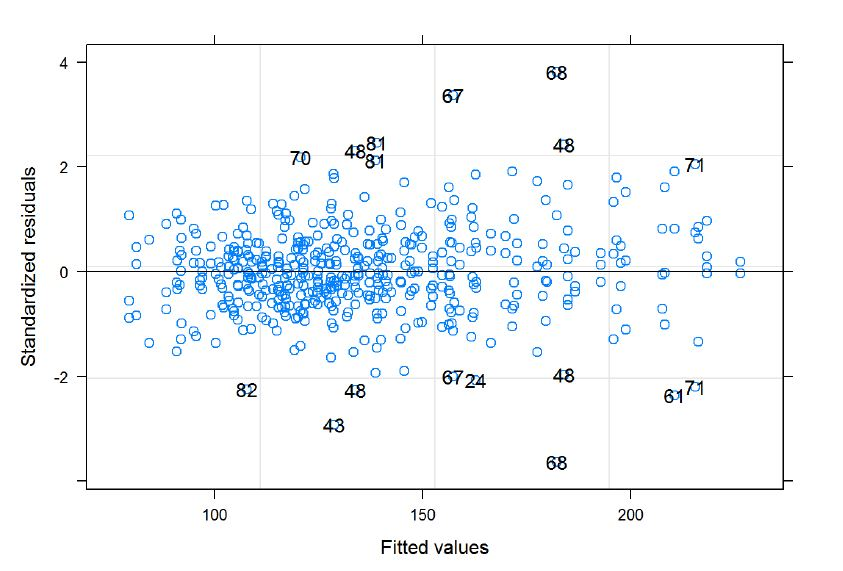
\includegraphics[width=0.8\linewidth]{images/Residuals-JS-Roy}
	\end{figure}
	
	The next figure depicts residual plot for the Systolic Blood Pressure example, panelled by the various measurement methods. It serves to confirm agreement between methods J and R, with lack of agreement between those two methods and method S. However, little insight can be gained as to what actually causes lack of agreement here. 
	\begin{figure}[h!]
		\centering
		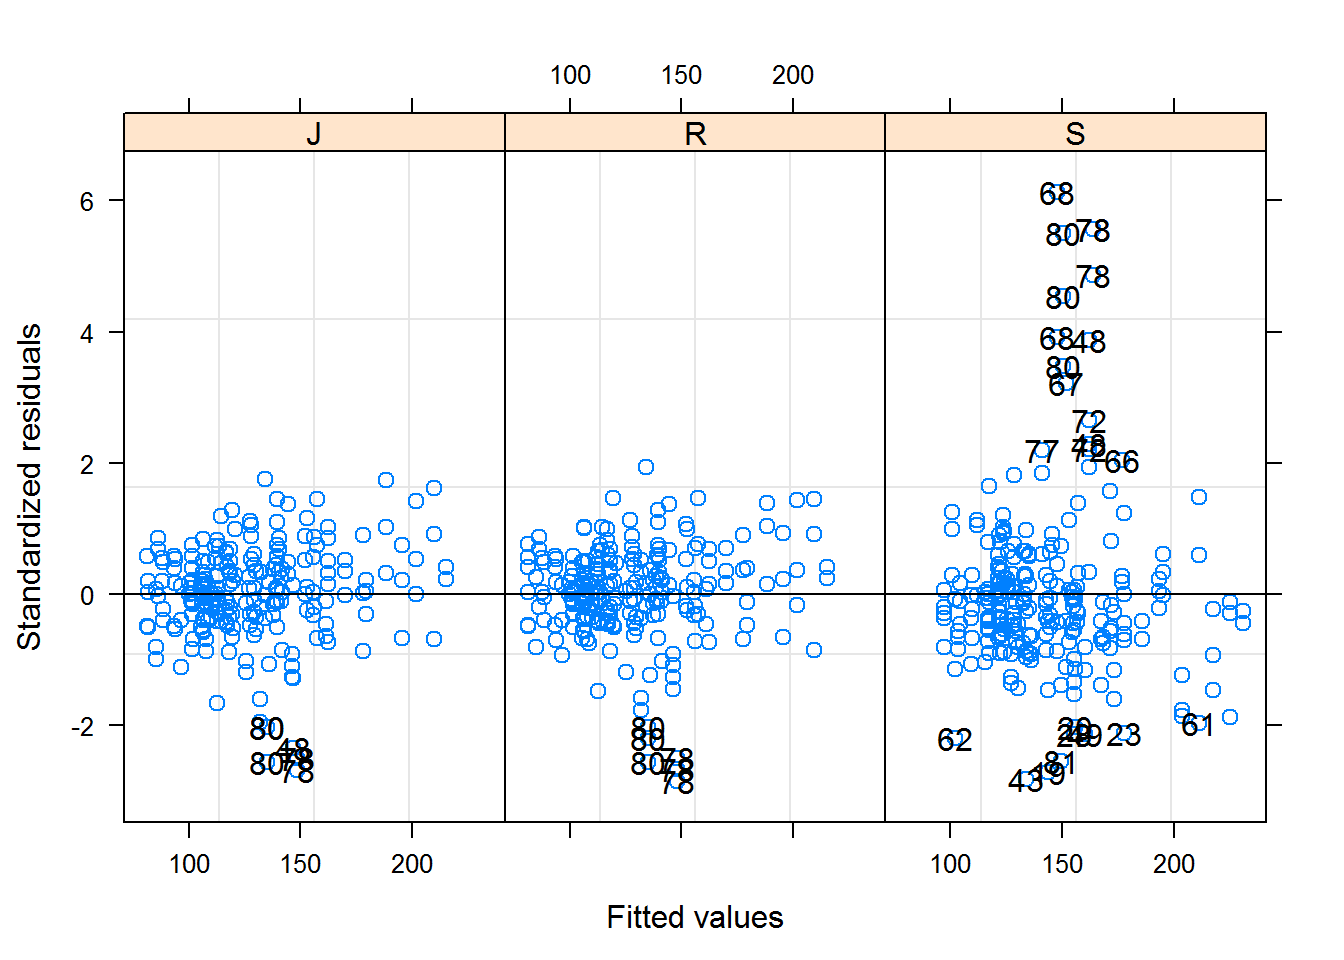
\includegraphics[width=0.8\linewidth]{images/bloodnlme-ResidPlot}
		\caption{LME Residuals by Method (Blood Pressure Data)}
		
	\end{figure}
	
	
	\newpage			
	\section{Influence Diagnostics}
	
	Model diagnostic techniques can determine whether or not the distributional assumptions are satisfied, but also to assess the influence of unusual observations. 
	
	
	Following model specification and estimation, it is of interest to explore the model-data
	agreement by raising pertinent questions. Pinheiro and Bates provide some insight into how to compute and interpret model diagnostic plots for LME models. Unfortunately this aspect of LME theory is not as expansive as the corresponding body of work for Linear Models. Their particular observations will be reverted to shortly. Further to the analysis of residuals, \citet{schabenberger} recommends the examination of the following questions:
	\begin{itemize}
		\item Does the model-data agreement support the model assumptions?
		\item Should model components be refined, and if so, which components? For example, should certain explanatory variables
		be added or removed, and is the covariance of the observations properly specified?
		\item Are the results sensitive to model and/or data? Are individual data points or groups of cases particularly
		influential on the analysis?
	\end{itemize}
	
	The last of these three questions, regarding influential points, is of particular interest in the context of Method Comparison. After fitting an LME model, it is important to carry put model diagnostics to check whether distributional assumptions for the
	residuals as satisfied and whether the fit the model is sensitive to unusual assumptions. The process of carrying out model
	diagnostic involves several informal and formal techniques, which will mentioned throughout the chapter.
	
	Influential points have a large influence on the fit of the model. Influential points are a set of one or more observations whose removal would cause a different conclusion in the analysis, e.g. substantially changes the estimate of the regression coefficients. \citet{west} remarks that influence diagnostics play an important role in the interpretation of results, because influential data can negatively 
	influence the statistical model and generalizability of the model.
	\citet{schabenberger} remarks that the concept of critiquing the model-data agreement applies in mixed models in the same way as in linear
	fixed-effects models. In fact, because of the more complex model structure, you can argue that model and
	data diagnostics are even more important \citep{west}.
	%Influential points have a large influence on the fit of the model. 
	
	%One approach for determining influential points is to compare the fit of the model with and without each observation.
	
	%The basic rationale behind identifying influential data is that when iteratively single units are omitted from the data, models based on these data should not produce substantially different estimates. 
	\subsection{A Procedure for Quantifying Influence}  
	
	\citet{schabenberger} describes a simple procedure for quantifying influence for LME Models. Firstly a model should be fitted to the data, and
	estimates of the parameters should be obtained. The second step is that either single or multiple data points, specifically outliers,
	should be omitted from the analysis, with the original parameter estimates being updated. This is known as \textit{leave one out} or \textit{leave k out} analysis. The final step of the procedure is comparing the sets of estimates computed from the entire and reduced data sets to determine whether the absence of observations changed the
	analysis. 
	
	
	%http://support.sas.com/documentation/cdl/en/statug/63033/HTML/default/viewer.htm#statug_mixed_sect024.htm
	
	%\subsubsection{Outliers and Leverage}
	Influence can be thought of as consequence of leverage and outlierness. Outliers are the most noteworthy data points in an analysis, and an objective of influence analysis is how influential they are, and the manner in which they are influential. They can point to a model breakdown and lead to development of a better model.
	The linear mixed effects model is a useful methodology for fitting a wide range of models. However, linear mixed effects models are known to be sensitive to outliers. Specifically likelihood based estimation techniques, such as ML and REML, are sensitive to outliers. \citet{Christensen} advises that identification of outliers is necessary before conclusions may be drawn from the fitted model. The leverage of an observation is a further consideration. 
	
	%The question of whether or not a point should be considered an outlier must therefore be addressed. An outlier is an observation whose true value is unusual given its value on the predictor variables.
	
	An observation with an extreme, but not unusual, value on a predictor variable is a point with high leverage. High leverage points can have a great amount of effect on the estimate of regression coefficients. In general. a high leverage point means a extreme value for the one or more of the independent variables, and a greater potential of overly influencing the final fitted model. However, if a case has  extreme values for the independent variables but is fitted very well by a regression model, this case is not necessarily overly influential.
	
	In classical linear models, leverages are the diagonal elements $h_{ii}$ of the Projection matrix, also known as the Hat Matrix $\boldsymbol{H}$. \citet{schabenberger} describes two analogues of $\boldsymbol{H}$ for LME models. However the practical use for either approach is not made clear.
	
	
	% - Leverage is a measure of how far an independent variable deviates from its mean.
	
	
	%\subsection{Cook's 1986 paper on Local Influence}%1.7.1
	
	\subsection{Analyzing Influence in LME models}
	
	Model diagnostic techniques, well established for classical models, have since been adapted for use with linear mixed effects models. Diagnostic techniques for LME models are inevitably more difficult to implement, due to the increased complexity.
	
	Influence diagnostics are formal techniques allowing for the identification of observations that exert substantial  influence on the estimates of fixed effects and variance covariance parameters.
	While linear models and GLMS can be studied with a wide range of well-established diagnostic technqiues, the choice of methodology is much more restricted for the case of LMEs. However
	influence diagnostics for LME Models is an area of active research. Research on diagnostic analyses for LME models are presented in \citet{Beckman}, 
	\citet{Christensen}, \citet{HildenMinton}, \citet{lesaffre1998local}, \citet{Banerjee1997}, 
	\citet{fung2002}, \citet{Demi}, \citet{Zewotir}, \citet{zewotir2008} and \citet{NobreSinger2007, NobreSinger2011}.
	
	
	
	
	
	\citet{schabenberger} states that goal of influence analysis is not primarily to mark data
	points for deletion so that a better model fit can be achieved for the reduced data, although this might be a
	result of influence analysis. The goal is rather to determine which cases are influential and the manner in
	which they are important to the analysis. 
	
	
	
	%For example, you are not only concerned with capturing the fixed and random components of the model. The LME model structure presents unique and interesting challenges that prompt us to reexamine the traditional ideas of influence and residual analysis.
	%
	
	
	
	
	
	
	
	
	%============================================================================================== %
	%Influence arises at two stages of the LME model. Firstly when $V$ is estimated by $\hat{V}$, and subsequent
	%estimations of the fixed and random regression coefficients $\beta$ and $u$, given $\hat{V}$.
	%
	%Diagnostic methods for fixed effects are generally analogues of methods used in classical linear models.
	%Diagnostic methods for variance components are based on `one-step' methods. 
	
	%======================================================= %
	\subsection{Measuring of Influence for LME Models}
	%- (Zewotir) 
	Influence analysis methodologies have been used extensively in classical linear models, and provided the basis for methodologies for use with LME models. Computationally inexpensive diagnostics tools have been developed to examine the issue of influence \citep{Zewotir}. 
	
	
	\citet{Zewotir} remarks the development of efficient computational formulas is crucial making deletion diagnostics useable, allowing one to obtain the \index{case deletion diagnostics} case deletion diagnostics by making use of basic building blocks, computed only once for the full model. A number of approaches to model diagnostics are described, including variance components, dixed effects parameters, prediction of the response variable and of random effects, and the likelihood function. Influence statistics can be grouped by the aspect of estimation that is their primary target:
	\begin{itemize}
		\item \textbf{overall measures compare changes in objective functions}: (restricted) likelihood distance (Cook and Weisberg 1982, Ch. 5.2)
		\item \textbf{influence on parameter estimates}: Cook's  (Cook 1977, 1979), MDFFITS (Belsley, Kuh, and Welsch 1980, p. 32)
		\item \textbf{influence on precision of estimates}: CovRatio and CovTrace
		\item \textbf{influence on fitted and predicted values}: PRESS residual, PRESS statistic (Allen 1974), DFFITS (Belsley, Kuh, and Welsch 1980, p. 15)
		\item \textbf{outlier properties}: internally and externally studentized residuals, leverage
	\end{itemize}
	
	
	\citet{Zewotir} lists several established methods of analyzing influence in LME models. These methods include Cook's distance for LME models,
	\index{likelihood distance} likelihood distance,
	the variance (information) ration,
	the \index{Cook-Weisberg statistic} Cook-Weisberg statistic, and
	the \index{Andrews-Prebigon statistic} Andrews-Prebigon statistic.
	
	The subscript $(U)$ is used to denote quantities computed from data with subset of cases $U$ omitted.
	If the global measure suggests that the points in $U$ are influential, you should next determine the nature of
	that influence. In particular, the points can affect
	\begin{itemize}
		\item the estimates of fixed effects
		\item the estimates of the precision of the fixed effects
		\item the estimates of the covariance parameters
		\item the estimates of the precision of the covariance parameters
		\item fitted and predicted values
	\end{itemize}	
	
	For example, if observations primarily affect the precision of the covariance parameters without exerting much influence on the fixed effects, then their presence in the data may not distort hypothesis
	tests or confidence intervals about $\beta$. 
	\citet{schabenberger} notes that removing observations or sets of observations affects fixed effects and covariance parameter estimates.
	
	
	
	
	
	\subsection{Deletion Diagnostics}
	
	%Data from single individuals, or a small group of subjects may influence non-linear mixed effects model selection. 
	%Diagnostics routinely applied in model building may identify such individuals, but these methods are not specifically designed for that purpose and are, therefore, not optimal. 
	%We describe two likelihood-based diagnostics for identifying individuals that can influence the choice between two competing models.
	
	
	Deletion diagnostics provide a means of assessing the influence of an observation (or groups of observations) on parameters inferences for a fitted model. For classical linear models, \citet{cook77} greatly expands the study of residuals and influence measures. The key to making deletion diagnostics useable is the development of efficient computational formulas, allowing one to obtain the \index{case deletion diagnostics} case deletion diagnostics by making use of basic building blocks, computed only once for the full model.
	Cook's key observation was the effects of deleting each observation in turn could be calculated with little additional computation. Cook proposed a measure that combines the information of leverage and residual of the observation, now known simply as the Cook's Distance, $D_{(i)}$, which can be calculated without fitting a new regression coefficient each time an observation is deleted. Consequently deletion diagnostics have become an integral part of assessing linear models.
	
	
	
	It must be pointed out that the effect on the precision of estimates is separate from the effect on the point estimates. Data points that have a small \index{Cook's distance}Cook's distance, for example, can still greatly affect hypothesis tests and confidence intervals, if their 
	influence on the precision of the estimates is large.	
	
	\citet{Christensen} notes the case deletion diagnostics techniques have not been applied to linear mixed effects models and seeks to develop methodologies in that respect. \citet{Christensen} developed their global influences for the deletion of single observations in two steps: a one-step estimate for the REML (or ML) estimate of the variance components, and an ordinary case-deletion diagnostic for a weighted resgression problem (conditional on the estimated covariance matrix) for fixed effects.
	
	The computation of case deletion diagnostics in the classical model is made simple by the fact that estimates of $\beta$ and $\sigma^2$, which exclude the $i$th observation, can be computed without re-fitting the model. Such update formulas are available in the mixed model only if you assume that the covariance parameters are not affected by the removal of the observation in question. This is rarely a reasonable assumption, and undermines the use of many proposed procedures for Method Comparison.
	
	\subsection{Cook's Distance}
	As previously described, \index{Cook's Distance} Cooks Distance ($D_{i}$) is a diagnostic technique used in classical linear models, that functions as an overall measure of the influence of an observation that is a measure of aggregate impact of each observation on the group of regression coefficients, as well as the group of fitted values. \index{Cook's distance} Cook's Distance as a measure of the influence of observations in subset $U$ on a vector of parameter estimates is given below \citep{cook77}
	\[ \delta_{(U)} = \hat{\beta} - \hat{\beta}_{(U)}.\]
	Observations, or sets of observations, that have high Cook's distance usually have high residuals, although this is not necessarily the case.
	
	
	%Cook's Distance is proportional to the sum of the squared differences between predictions made with all observations in the analysis and predictions made leaving out the observation in question.
	If the predictions are the same with or without the observation in question, then the observation has no influence on the regression model. If the predictions differ greatly when the observation is not included in the analysis, then the observation is influential.
	
	%======================================================================================= %
	
	
	Large values for Cook's distance indicate observations for special attention. Cook's distance can be used in several ways: to indicate data points that are particularly worth checking for validity; to indicate regions of the design space where it would be good to be able to obtain more data points.
	
	
	
	Use of threshold values for Cook's Distance is discouraged \citep{fox1997}. However, informal heuristics do exist for OLS models; Obervations for which Cook's distance is higher than 1 are usually considered as influential. Another informal threshold of $4/n$ or $4/(n-k-1)$, where $n$ is the number of observations and $k$ the number of explanatory variables.
	\citet{fox1997} advises the use of diagnostic plotting and to examine in closer details the points with \textit{``values of D that are substantially larger than the rest}", and that thresholds should feature only to enhance graphical displays.
	
	
	The effect on the precision of estimates is separate from the effect on the point estimates. Data points that have a small \index{Cook's distance}Cook's distance, for example, can still greatly affect hypothesis tests and confidence intervals, if their  influence on the precision of the estimates is large.
	
	
	\citet{Christensen} develops \index{case deletion diagnostics} case deletion diagnostics, in particular the equivalent of \index{Cook's distance} Cook's distance for diagnosing influential observations when estimating the fixed effect parameters and variance components, adapting the \index{Cook's distance}Cook's Distance measure for the analysis of LME models. For LME models, two formulations exist; a \index{Cook's distance}Cook's distance that examines the change in fixed fixed parameter estimates, and another that examines the change in random effects parameter estimates. The outcome of either Cook's distance is a scaled change in either $\beta$ or $\theta$. \citet{Zewotir} gives a detailed discussion of the various formulation for Cook's distances for LME Models.
	
	\begin{figure}[h!]
		\centering
		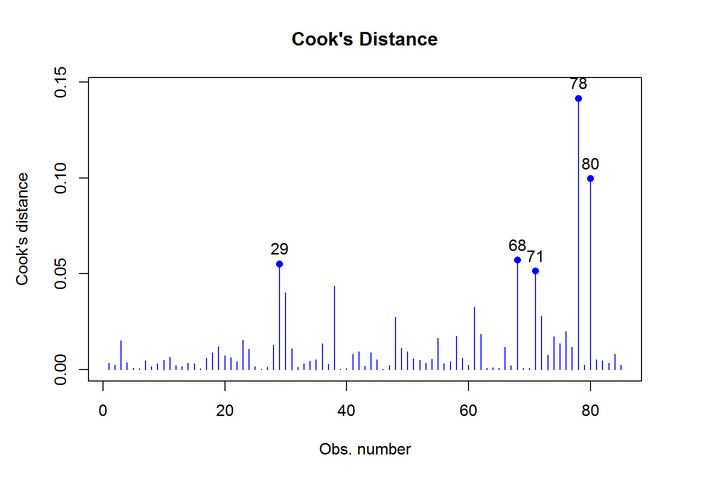
\includegraphics[width=0.7\linewidth]{images/CooksDistancePlot-JS-Roy}
		\caption{}
		\label{fig:CooksDistancePlot-JS-Roy}
	\end{figure}	
	%	For LME models, Cook's distance can be extended to model influence diagnostics by defining:
	%	\[ C_{\beta i} = {(\hat{\beta} - \hat{\beta}_{[i]})^{T}(\boldsymbol{X}^{\prime}\boldsymbol{V}^{-1}\boldsymbol{X}) (\hat{\beta} - \hat{\beta}_{[i]}) \over p}\]
	%	
	%	It is also desirable to measure the influence of the case deletions on the covariance matrix of $\hat{\beta}$.
	
	%	It uses the same structure for measuring the combined impact of the differences in the estimated regression coefficients when the $i$th case is deleted. Importantly, $D_{(i)}$ can be calculated without fitting a new regression coefficient each time an observation is deleted.
	
	%Cook's Distance is proportional to the sum of the squared differences between predictions made with all observations in the analysis and predictions made leaving out the observation in question.
	
	
	
	
	%
	%	
	%	If V is known, Cook's D can be calibrated according to a chi-square distribution with degrees of freedom equal to the rank of $\boldsymbol{X}$ \citep{cpj92}.
	%	
	%	
	
	
	
	
	
	
	
	
	
	
	
	%		
	%		
	%		In this section we introduce influence analysis and case deletion diagnostics. A full overview of the topic will be provided although there are specific tools that are particularly useful in the case of Method Comparison problems: specifically the Cook's Distance and the DFBETA.
	
	
	
	
	Consideration of how leave-$U$-out diagnostics would work in the context of Method Comparison problems is required. There are several scenarios. \citet{preisser} describes two type of diagnostics. When the set consists of only one observation, the type is called
	`\textit{observation-diagnostics}'. For multiple observations, Preisser describes the diagnostics as `\textit{cluster-deletion}' diagnostics. Suppose we have two methods of measurement X and Y, each with three measurements for a specific case: $(x_1,x_2,x_3,y_1,y_2,y_3)$
	
	\begin{itemize}
		\item Leave One Out - one observation is omitted (e.g. $x_1$)
		\item Leave Pair Out - one pair of observation  is omitted (e.g. $x_1$ and $y_1$)
		\item Leave Case (or Item or Subject) Out - All observations associated with a particular case or subject are omitted. (e.g. $\{x_1,x_2,x_3,y_1,y_2,y_3\}$)
	\end{itemize}
	%% Schabenberger
	%%
	
	The natural sampling unit is the item or subject, similar to the example provided by \citet{schabenberger}. Hence, the third option, henceforth, referred to as ``Leave subject Out" will be the option used.
	
	
	\subsection{Local Influence}
	\citet{cook86} gives a completely general method for assessing the influence of local departures from assumptions in statistical models, introducing methods for local influence assessment for classical linear models. These methods provide a powerful tool for examining perturbations in the assumption of a model, particularly the effects of local perturbations of parameters of observations. The local-influence approach to influence assessment is quite different from the case deletion approach, comparisons are of interest.
	
	% % Beckman, Nachtsheim and Cook (1987)
	\citet{Beckman} applied the \index{local influence}local influence method of Cook (1986) to the analysis of the LME model.  Other authors such as \citet{lesaffre1998local} have also extended these idea to LME models. 
	While the concept of influence analysis is straightforward, implementation in mixed models is more complex. Update formulae for fixed effects models are available only when the covariance parameters are assumed to be known. As such the local influence approach are not particularly useful in the context of Method Comparison, and so will not be considered further.
	
	
	
	
	
	\subsection{Comparing Influence and Residual Analysis}
	%In LME models, there are two types of residuals, marginal residuals and conditional residuals. A
	%marginal residual is the difference between the observed data and the estimated marginal mean. A conditional residual is the
	%difference between the observed data and the predicted value of the observation. In a model without random effects, both sets of residuals coincide \citep{schab}.
	
	\citet{influenceLME4} compares residual analysis and influence analysis. Cases with high residuals (defined as the difference between the observed and the predicted scores on the dependent
	variable) or with high standardized residuals (defined as the residual divided by the standard deviation
	of the residuals) are indicated as outliers.
	
	However, an influential case is not necessarily an outlying residual. On the contrary: a strongly influential case dominates
	the regression model in such a way, that the estimated regression line lies closely to this case. The analysis of residuals cannot be used for the detection of influential cases \citep{crawley2012r}.
	
	
	
	
	
	
	%\subsection{Extension of Diagnostic Methods to LME models}
	
	
	
	
	
	
	%============================================================================================================================ %
	
	
	\subsection{Iterative and Non-Iterative Influence Analysis}
	
	
	
	
	%----schabenberger page 8
	For linear models, the implementation of influence analysis is straightforward, but for LME models the process is more complex. \citet{schabenberger} examines the use and implementation of
	influence measures in LME models. \citet{schabenberger} highlights some of the issue regarding implementing LME model diagnostics, describing  the choice between \index{iterative influence analysis} iterative influence analysis and \index{non-iterative influence analysis} non-iterative influence analysis.
	\citet{schabenberger} considers several important aspects of the use and implementation of influence measures in LME models, noting that it is not always possible to
	derive influence statistics necessary for comparing full- and reduced-data parameter estimates. Closed-form expressions for computing the change in important model quantities might not be available.
	
	On a related matter, \citet{schabenberger} describes the scenario wherein a data point is removed and the new estimate of the $D$ matrix is not positive definite. This may occur if a variance component
	estimate now falls on the boundary of the parameter space \citep{schabenberger}. 
	
	%%Non-Iterative
	For classical linear models, it is not necessary to refit the model after removing a data point in order to measure the impact of an observation on the model. The change in fixed effect estimates, residuals, residual sums of squares, and the variance-covariance matrix of the fixed effects can be computed based on the fit to the full data alone, using update formulas \citep{sherman, hager1989}.
	
	
	
	However, in LME models several important complications arise. Data points can affect not only the fixed effects but also the covariance parameter estimates on which the fixed-effects estimates depend.
	
	When applied to LME models, such update formulas are available only if one assumes that the covariance parameters are not affected by the removal of the observation in question. However, this is rarely a reasonable assumption.
	For LME models, non-iterative methods are computationally efficient, but require the rather strong assumption that all 
	covariance parameters are known, and thus are not updated, with the exception of the profiled residual variance.
	Update formulas for ``leave-U-out" estimates typically fail to account for changes in covariance parameters.  As the influence that each item would have on the variance estimate of a method comparison model is crucial, this substanitally negates their usefulness for Roy's Model.
	
	%============================================%
	%%Iterative
	Iterative influence diagnostics requiring fitting the model without the observations in question. Computation execution time is substantially longer, although this is balanced by algorithmic 
	simplicity, with no assumptions beyond those used for the original model. A measure of total influence requires updates of all model parameters. This can only be achieved in general is by omitting observations or cases, then refitting the model. 
	
	
	An iterative analysis may seem computationally expensive. Computing iterative influence diagnostics for $n$ observations
	requires $n+1$ mixed models to be fitted iteratively.
	The execution times for iterative procedures are longer relative to non-iterative procedures, but are not so long that they would dissuade an analyst from using them.
	Despite the addition execution time of iteratives
	approaches, they are preferable for Method Comparison problems, as they can facilitate several complementary analyses concurrently. 
	
	
	Iterative methods retain the potential for useful analyses, if applied at different stage of the modelling process. Diagnostic measures, specifically the DFBETA, have characteristics that would make them very useful at the exploratory stage of the method comparison process. Implicitly various assumptions about variance are used, but simultaneously an approach based on DFBETA can be used to assess if these assumptions are valid.
	
	
	
	\subsection{Likelihood Distance}
	An overall influence statistic measures the change in the objective function being minimized. For example, in
	classical linear, the residual sums of squares serves that purpose. In linear mixed models fit by
	\index{maximum likelihood} maximum likelihood (ML) or \index{restricted maximum likelihood} restricted maximum likelihood (REML), an overall influence measure is the \index{likelihood distance} likelihood distance \citep{CookWeisberg}.
	
	%	\subsection{Likelihood Distances}
	
	The \index{likelihood distance} likelihood distance is a global summary measure that expresses the joint influence of the subsets of observations, $U$, on all parameters that were subject to updating. \citet{schabenberger} points out that the likelihood distance $LD(\psi_{(U)})$ is not the log-likelihood obtained by fitting the model to the reduced data set. Instead it is obtained by evaluating the likelihood function based on the full data set (containing all $n$ observations) at the reduced-data estimates.
	
	
	
	
	%==========================================================%
	%	\subsubsection{Likelihood Distances}
	
	The
	procedure requires the calculation of the full data estimates
	$\hat{\psi}$ and estimates based on the reduced data set
	$\hat{\psi}_{(U)}$. The likelihood distance is given by
	determining
	\[
	LD_{(U)} = 2\{l(\hat{\psi}) - l( \hat{\psi}_{(U)}) \}\]\[
	RLD_{(U)} = 2\{l_{R}(\hat{\psi}) - l_{R}(\hat{\psi}_{(U)})\}
	\]
	Large values indicate that $\boldsymbol{\hat{\theta}}$ and $\boldsymbol{\hat{\theta}_\omega}$ differ considerably.
	
	\citet{west} examines a group of methods that examine various aspects of influence diagnostics for LME models. For overall influence, the most common approaches are the \textit{likelihood distance} and the \textit{restricted likelihood distance}.
	
	%For noniterative methods the following computational devices are used to compute (restricted) likelihood distances provided that the residual variance
	%$\sigma^2$ is profiled.
	
	
	\section{Model Diagnostics for Roy's Models}
	
	Further to previous work, this section revisits case-deletion and residual diagnostics, and explores how approaches devised by  \citet{Galecki} can be used to appraise Roy's model. These authors specifically look at Cook's Distances and Likelihood Distances.
	%	For the Roy Model, Cook's Distances may also be generated using the \textbf{\textit{predictmeans}}
	%	
	
	
	
	
	
	\begin{figure}[h!]
		\centering
		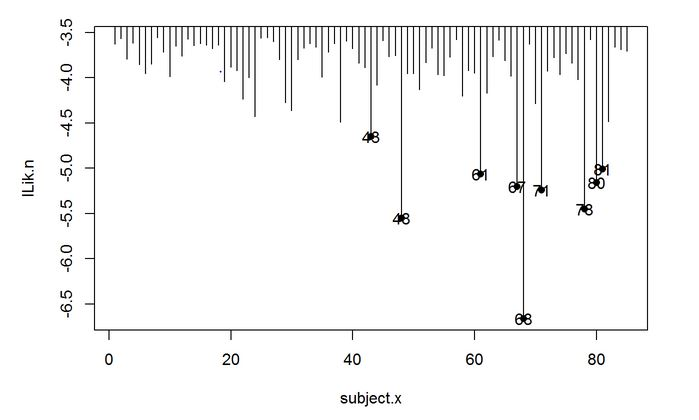
\includegraphics[width=0.7\linewidth]{images/LogLik-JS-Roy}
		\caption{}
		\label{fig:LogLik-JS-Roy}
	\end{figure}
	
	
	
	
	
	
	
	
	\subsubsection{Case Deletion Diagnostics for Variance Ratios}
	
	
	Taking the core principals of his methods, and applying them to the Method Comparison problem, case deletion diagnostics are used on the variance components of the Roy's model, specifically the ratio of between subject variances and the within subject covariances respecitvely.
	
	
	\[ \mbox{BSVR} = \frac{\sigma^2_2}{\sigma^2_2} \phantom{makespace}  \mbox{WSVR} = \frac{d^2_2}{d^2_2} \]
	
	These variance ratios are re-computed for each case removed, and may be analysed seperately or jointly for outliers.
	
	
	
	
	%\subsubsection{Methods for Identifying Outliers}
	The Grubbs' Test for Outliers is a commonly used technique for assessing outlier in a univariate data set, of which there are several variants.
	As there may be several outliers present, the Grubbs test is not practical. However an indication that a point being beyond the fences according to Tukey's specification for boxplots will suffice.
	
	
	% The first variant of Grubb's test is used to detect if the sample dataset contains one outlier, statistically different than
	% the other values. The test statistic is based by calculating score of this outlier $G$ (outlier minus mean and divided
	% by the standard deviation) and comparing it to appropriate critical values. Alternative method is calculating ratio of
	% variances of two datasets - full dataset and dataset without outlier.
	% %The obtained value called U is bound with G by simple formula.
	% The second variant is used to check if lowest and highest value are two outliers on opposite tails of sample. It is based on calculation of ratio of range to standard deviation of the sample.
	% 
	% The third variant calculates ratio of variance of full sample and sample without two extreme observations.
	% It is used to detect if dataset contains two outliers on the same tail.
	
	
	
	The WSVR values are plotted against the corresponding BSVR values, with commonly used bivariate methods may be applied jointly to the both sets of data sets, e.g Mahalanobis distances. Confidence ellipses can be superimposed over the plot with minimal effort. Two ellipses are generated by this technique, a 50 \% and 97.5\% confidence ellipse respectively. Outlying cases are idenified by the plot. Subject 68 is the most prominent case.
	
	The subjects were ranked by Mahalanobis distance, with the top 10 being presented in the following table. Both sets of ratio are addtionally expressed as a ratio of the full model variance ratios.
	\begin{center}
		\begin{tabular}{|c|c|c|c|c|c|}
			\hline
			Subject (u) &  MD & WSVR$_{(u)}$ & WSVR (\%) & BSVR$_{(u)}$   & BSVR (\%)     \\ \hline \hline
			68 & 44.7284   & 1.3615  & 0.9132   & 1.0353  & 0.9849 \\ \hline
			30 & 16.7228   & 1.5045  & 1.0092   & 1.1024  & 1.0487 \\ \hline
			71 & 11.5887   & 1.5210  & 1.0202   & 1.0932  & 1.0400 \\ \hline
			80 & 11.0326   & 1.4796  & 0.9925   & 1.0114  & 0.9621 \\ \hline
			38 & 10.3671   & 1.5011  & 1.0069   & 1.0917  & 1.0385 \\ \hline
			67 & 10.1940   & 1.4308  & 0.9598   & 1.0514  & 1.0002 \\ \hline
			43  & 7.6932   & 1.4385  & 0.9649   & 1.0511  & 0.9999 \\ \hline
			72  & 4.7350   & 1.4900  & 0.9995   & 1.0262  & 0.9762 \\ \hline
			48  & 4.4321   & 1.4950  & 1.0028   & 1.0280  & 0.9779 \\ \hline
			29  & 4.3005   & 1.4910  & 1.0001   & 1.0769  & 1.0244 \\ \hline
		\end{tabular}
	\end{center}
	From this table one may conclude that subjects 72, 48 and 29 are not particularly influential. Interestingly Subject 78, which was noticeable in the case deletion diagnostics for fixed effects, does not feature in this table.
	
	\begin{figure}[h!]
		\centering
		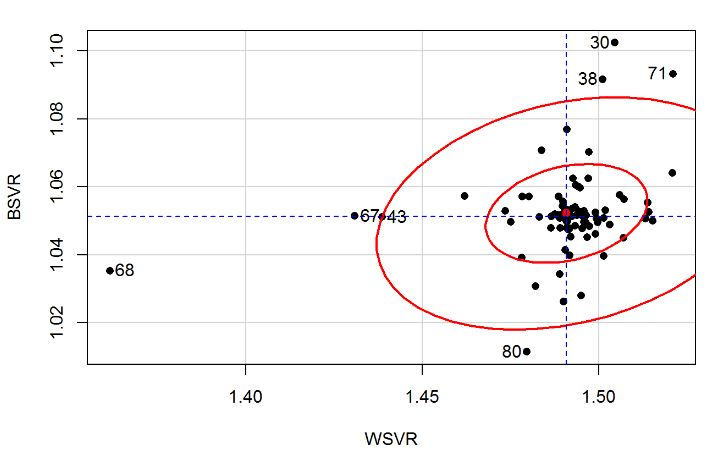
\includegraphics[width=0.9\linewidth]{08-plot1}
		\caption{}
		\label{fig:08-plot1}
	\end{figure}
	
	
	
	%===========================================================================%
	
	\subsubsection{Variance Ratios}
	
	The relationship between precision and the within-item and between-item variability must be established. Roy establishes the equivalence of repeatability and within-item variability, and hence precision.  The method with the smaller within-item variability can be deemed to be the more precise.
	
	A useful approach is to compute the confidence intervals for the ratio of within-item standard deviations (equivalent to the ratio of repeatability coefficients), which can be interpreted in the usual manner.
	%	
	
	Pinheiro and Bates (pg 93-95) give a description of how confidence intervals for the variance components are computed. Furthermore a complete set of confidence intervals can be computed to complement the variance component estimates.
	
	What is required is the computation of the variance ratios of within-item and between-item standard deviations.
	
	A naive approach would be to compute the variance ratios by relevant F distribution quantiles. However, the question arises as to the appropriate degrees of freedom.
	Bootstrap methods for computing confidence intervals may be considered.
	
	
	
	
	
	
	
	\section{Using DFBETAs from LME Models to Assess Agreement}
	
	The impact of an observation on a regression fitting can be determined by the difference between the estimated regression coefficient of a model with all observations and the estimated coefficient when the particular observation is deleted. DFBETA and DFFITS are well known measures of influence. Emphasis shall be placed on DFBETA, but a brief discussion of DFFITS is merited as it potentially provides for useful techniques in method comparison. \citet{schabenberger} provides a mathematical desciption of both.
	
	DFBETAS is a standardized measure of the absolute difference between the estimate with a particular
	case included and the estimate without that particular case,, thus measuring the impact each observation has on a particular predictor \citep{belsley2005}. For LME models, the DFBETA is a measure that standardizes the absolute difference in parameter estimates between an LME model based on a full set of data, and a model from reduced data.
	
	
	
	
	In general, large values of DFBETAS indicate observations that are influential in estimating a given parameter. \citet{belsley2005} recommend 2 as a general cutoff value to indicate influential observations and as a size-adjusted cutoff. There is no agreement as to the critical threshold for DFBETAs. The cut-off value for DFBETAs is $\frac{2}{\sqrt{n}}$, where $n$ is the number of observations. However, another cut-off is to look for observations with a value greater than 1.00. Here cutoff means,
	``this observation could be overly influential on the estimated coefficient".
	
	DFFITS is a diagnostic meant to show how influential a point is in a statistical regression. It is defined as the change, in the predicted value for a point, obtained when that point is left out of the regression, divided by the estimated standard deviation of the fit at that point:
	
	
	
	
	
	
	\subsubsection{DFBETAs for Method Comparison}
	
	For LME models, a value for DFBETAS is calculated for each of the $k$ fixed effects, and for each of the $n$ item. Correctly there will be $p+1$ DFBETAs (the intercept, $\beta_0$, and one $\beta$ for each covariate). When the LME model is specified without an intercept term, as in Roy's Model, there is a set of DFBETAs corresponding to each measurement method, hence an $n \times p$ matrix.
	
	In the case of method comparison studies, a series of scatterplots can be constructed to compare each pair of measurement methods.
	Furthermore 95\% confidence ellipse can be constructed around these scatterplots.
	
	
	
	The LME approach proposed by \citet{ARoy2009} is constrained by computational tractability.
	Consequently a simpler LME formulation is used, one similar to that of \citet{BXC2008}. However one constraint that can be dispensed with is the restriction to
	two methods of measurement: we can now use any number of methods.
	The benefit of using this model is that metrics such as Cook's Distance and DFBETAs can be computed also.
	
	Furthermore, these measures form the basis of the analysis, rather than the estimates derived from the model. In the context of method comparison, these variables are the methods of measurement.
	Agreement will considered in the context of inter-method bias and the within-item variance ratio. Between-item variance ratio is not considered for this analysis.
	
	For a Method Comparison study, DFBETAs can be used as a proxy measurement, allowing simple techniques to be used for assessing agreement. Suppose an LME model was formulated to model agreement for two or more methods of measurement, specifically with replicate measurements. If the methods are to be agreement, the DFBETAs for each case would be the same for both methods. As such, agreement between any two methods can be determined by a simple scatterplot of the DFBetas. 
	
	
	If the lack of agreement is caused, in part or in full, by differing within-item variances, there would be differing DFBETAs for each pair of methods. If the points align along the line of equality, then both methods can be said to be in agreement for within item variance. However DFBETAs are not useful for determining inter-method bias. If there is good agreement between methods, or if lack of agreement is caused by inter-method bias only, the DFBETA values will be almost identical for each subject in the data set. 
	
	Following the idea proposed by \citet{BA86}, an identity plot to visually inspect this relationship between sets of DFBETAs. Modern statistical software usually allows for the creation of co-plots, so a grid of identity plots may be easily rendered for comparing each pair of methods. Used in conjection with a Bland-Altman plot, this co-plot can quickly determine agreement and indicate the source of lack of agreement.
	
	For an LME model fitted to the Blood data, the results tabulated below can be produced.  Cases can be ranked by the Cook's Distance, such that the most divergent DFBETA are highlighted, with the top 6 being presented below). The remaining columns are the DFBeta for each of the fixed effects, for each of the 85 subject.
	\begin{center}
		\begin{tabular}{|c|c|c|c|c|} \hline
			Subject &    Cook's D  &    Method J  &   Method R  & Method S \\ \hline \hline
			78 & 0.61557407 & -0.02934556 & -0.03387780 & 0.2954937  \\ \hline
			80 & 0.41590973 & -0.06305026 & -0.06515241 & 0.2123881  \\ \hline
			68 & 0.22536651 & -0.05334867 & -0.05062375 & 0.1555187  \\ \hline
			72 & 0.09348500  & 0.02388626  & 0.02419887 & 0.1617474  \\ \hline
			48 & 0.08706988  & 0.02147541  & 0.03145273 & 0.1581591  \\ \hline
			30 & 0.07118415  & 0.26925807  & 0.26215970 & 0.1581569  \\ \hline
		\end{tabular}
	\end{center}
	For DFBETA identity plots are presented below. This set of plots indicate agreement between methods J and R in terms of within-item variance, while severe lack of agreement exists between these methods and the third method S, as is the conclusion of \citet{ARoy2009}.	
	\begin{figure}[h!]
		\centering
		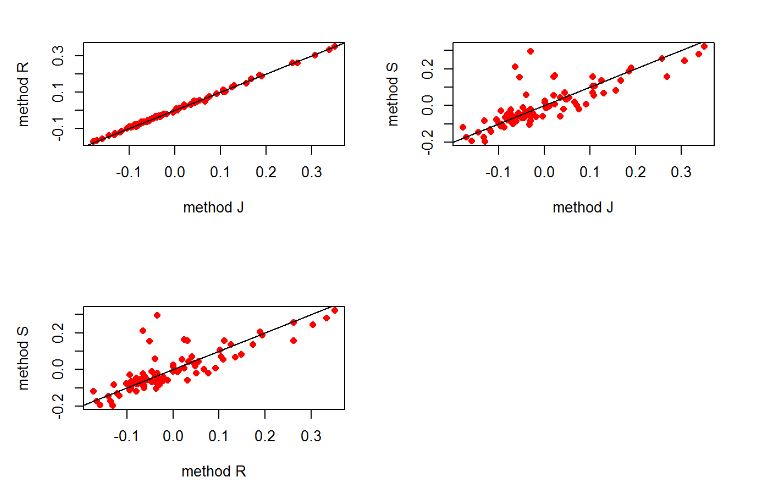
\includegraphics[width=1\linewidth]{images/04-DFbetaplots}
		% \caption{}
		% \label{fig:04-DFbetaplots}
	\end{figure}
	
	If lack of agreement is indicated, a subsequent analysis using a technique proposed by \citet{ARoy2009} can be used to identify the specific cause for this lack of agreement.
	
	Other analyses may be used to complement these plots. The Pearson Correlation coefficient of the DFBETAs can be used in conjection with this analysis. A high correlation confirms good agreement, thouhg no threshold value for agreement is suggested.
	
	The Bonferroni Outlier Test and Cook's Distance values can be used to identify unusual cases, when the relationship between sets of DFBETA is modelled as a (classical) linear model. In this model, the covariates should be homoskedastic. A test for non-constant variance may be used to verify this. 
	
	
	As an alternative to scatterplots, a mean difference plot could be used to assess agreement of with-item variance. This mean-difference plot differs from the Bland-Altman plot in that the plot is denominated in terms of DFBETA values, and not in measurement units. Here two of the three pairs of methods are compared on the same plot, red points indicate the J-R comparison while blue points are for the J-S comparison.
	
	\begin{figure}[h!
		]
		\centering
		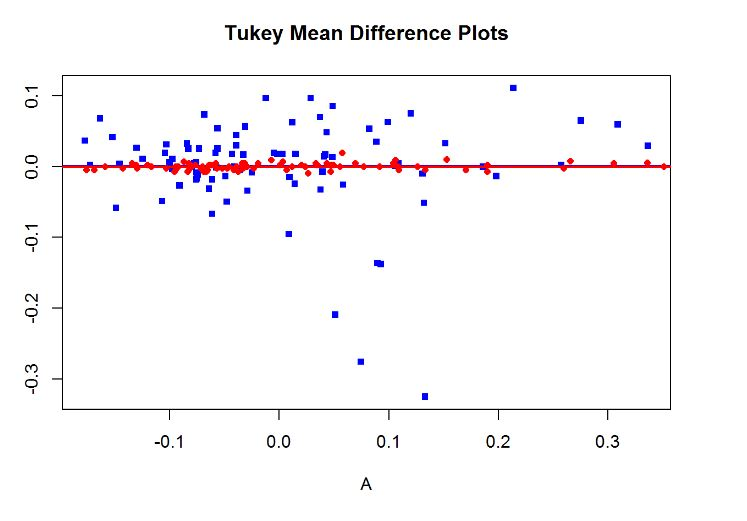
\includegraphics[width=0.7\linewidth]{images/04-TMDplot}
		
	\end{figure}
	
	%============================================== %


			
			\addcontentsline{toc}{section}{Bibliography}
			\bibliographystyle{chicago}
			\bibliography{DB-txfrbib}

\end{document}
